%&preformat-disser
\RequirePackage[l2tabu,orthodox]{nag} % Раскомментировав, можно в логе получать рекомендации относительно правильного использования пакетов и предупреждения об устаревших и нерекомендуемых пакетах
% Формат А4, 14pt (ГОСТ Р 7.0.11-2011, 5.3.6)
\documentclass[a4paper,14pt,oneside,openany]{memoir}

%%%%%%%%%%%%%%%%%%%%%%%%%%%%%%%%%%%%%%%%%%%%%%%%%%%%%%%
%%%% Файл упрощённых настроек шаблона автореферата %%%%
%%%%%%%%%%%%%%%%%%%%%%%%%%%%%%%%%%%%%%%%%%%%%%%%%%%%%%%

%%% Инициализирование переменных, не трогать!  %%%
\newcounter{showperssign}
\newcounter{showsecrsign}
\newcounter{showopplead}
%%%%%%%%%%%%%%%%%%%%%%%%%%%%%%%%%%%%%%%%%%%%%%%%%%%%%%%

%%% Список публикаций %%%
\makeatletter
\@ifundefined{c@usefootcite}{
  \newcounter{usefootcite}
  \setcounter{usefootcite}{0} % 0 --- два списка литературы;
                              % 1 --- список публикаций автора + цитирование
                              %       других работ в сносках
}{}
\makeatother

\makeatletter
\@ifundefined{c@bibgrouped}{
  \newcounter{bibgrouped}
  \setcounter{bibgrouped}{0}  % 0 --- единый список работ автора;
                              % 1 --- сгруппированные работы автора
}{}
\makeatother

%%% Область упрощённого управления оформлением %%%

%% Управление зазором между подрисуночной подписью и основным текстом %%
\setlength{\belowcaptionskip}{10pt plus 20pt minus 2pt}


%% Подпись таблиц %%

% смещение строк подписи после первой
\newcommand{\tabindent}{0cm}

% тип форматирования таблицы
% plain --- название и текст в одной строке
% split --- название и текст в разных строках
\newcommand{\tabformat}{plain}

%%% настройки форматирования таблицы `plain'

% выравнивание по центру подписи, состоящей из одной строки
% true  --- выравнивать
% false --- не выравнивать
\newcommand{\tabsinglecenter}{false}

% выравнивание подписи таблиц
% justified   --- выравнивать как обычный текст
% centering   --- выравнивать по центру
% centerlast  --- выравнивать по центру только последнюю строку
% centerfirst --- выравнивать по центру только первую строку
% raggedleft  --- выравнивать по правому краю
% raggedright --- выравнивать по левому краю
\newcommand{\tabjust}{justified}

% Разделитель записи «Таблица #» и названия таблицы
\newcommand{\tablabelsep}{~\cyrdash\ }

%%% настройки форматирования таблицы `split'

% положение названия таблицы
% \centering   --- выравнивать по центру
% \raggedleft  --- выравнивать по правому краю
% \raggedright --- выравнивать по левому краю
\newcommand{\splitformatlabel}{\raggedleft}

% положение текста подписи
% \centering   --- выравнивать по центру
% \raggedleft  --- выравнивать по правому краю
% \raggedright --- выравнивать по левому краю
\newcommand{\splitformattext}{\raggedright}

%% Подпись рисунков %%
%Разделитель записи «Рисунок #» и названия рисунка
\newcommand{\figlabelsep}{~\cyrdash\ }  % (ГОСТ 2.105, 4.3.1)
                                        % "--- здесь не работает

%Демонстрация подписи диссертанта на автореферате
\setcounter{showperssign}{1}  % 0 --- не показывать;
                              % 1 --- показывать
%Демонстрация подписи учёного секретаря на автореферате
\setcounter{showsecrsign}{1}  % 0 --- не показывать;
                              % 1 --- показывать
%Демонстрация информации об оппонентах и ведущей организации на автореферате
\setcounter{showopplead}{1}   % 0 --- не показывать;
                              % 1 --- показывать

%%% Цвета гиперссылок %%%
% Latex color definitions: http://latexcolor.com/
% \definecolor{linkcolor}{rgb}{0.9,0,0}
% \definecolor{citecolor}{rgb}{0,0.6,0}
% \definecolor{urlcolor}{rgb}{0,0,1}
\definecolor{linkcolor}{rgb}{0,0,0} %black
\definecolor{citecolor}{rgb}{0,0,0} %black
\definecolor{urlcolor}{rgb}{0,0,0} %black
            % общие настройки шаблона
%%% Проверка используемого TeX-движка %%%
\newif\ifxetexorluatex   % определяем новый условный оператор (http://tex.stackexchange.com/a/47579)
\ifxetex
    \xetexorluatextrue
\else
    \ifluatex
        \xetexorluatextrue
    \else
        \xetexorluatexfalse
    \fi
\fi

\newif\ifsynopsis           % Условие, проверяющее, что документ --- автореферат

\usepackage{etoolbox}[2015/08/02]   % Для продвинутой проверки разных условий
\providebool{presentation}

\usepackage{comment}    % Позволяет убирать блоки текста (добавляет
                        % окружение comment и команду \excludecomment)

%%% Поля и разметка страницы %%%
\usepackage{pdflscape}  % Для включения альбомных страниц
\usepackage{geometry}   % Для последующего задания полей

%%% Математические пакеты %%%
\usepackage{amsthm,amsmath,amscd}   % Математические дополнения от AMS
\usepackage{amsfonts,amssymb}       % Математические дополнения от AMS
\usepackage{mathtools}              % Добавляет окружение multlined
\usepackage{xfrac}                  % Красивые дроби
\usepackage[
    locale = DE,
    list-separator       = {;\,},
    list-final-separator = {;\,},
    list-pair-separator  = {;\,},
    list-units           = single,
    range-units          = single,
    range-phrase={\text{\ensuremath{-}}},
    % quotient-mode        = fraction, % красивые дроби могут не соответствовать ГОСТ
    fraction-function    = \sfrac,
    separate-uncertainty,
    ]{siunitx}[=v2]                 % Размерности SI
\sisetup{inter-unit-product = \ensuremath{{}\cdot{}}}

% Кириллица в нумерации subequations
% Для правильной работы требуется выполнение сразу после загрузки пакетов
\patchcmd{\subequations}{\def\theequation{\theparentequation\alph{equation}}}
{\def\theequation{\theparentequation\asbuk{equation}}}
{\typeout{subequations patched}}{\typeout{subequations not patched}}

%%%% Установки для размера шрифта 14 pt %%%%
%% Формирование переменных и констант для сравнения (один раз для всех подключаемых файлов)%%
%% должно располагаться до вызова пакета fontspec или polyglossia, потому что они сбивают его работу
\newlength{\curtextsize}
\newlength{\bigtextsize}
\setlength{\bigtextsize}{13.9pt}

\makeatletter
%\show\f@size    % неплохо для отслеживания, но вызывает стопорение процесса,
                 % если документ компилируется без команды  -interaction=nonstopmode
\setlength{\curtextsize}{\f@size pt}
\makeatother

%%% Кодировки и шрифты %%%
\ifxetexorluatex
    \ifpresentation
        \providecommand*\autodot{} % quick fix for polyglossia 1.50
    \fi
    \PassOptionsToPackage{no-math}{fontspec}    % https://tex.stackexchange.com/a/26295/104425
    \usepackage{polyglossia}[2014/05/21]        % Поддержка многоязычности
                                        % (fontspec подгружается автоматически)
\else
   %%% Решение проблемы копирования текста в буфер кракозябрами
    \ifnumequal{\value{usealtfont}}{0}{}{
        \input glyphtounicode.tex
        \input glyphtounicode-cmr.tex %from pdfx package
        \pdfgentounicode=1
    }
    \usepackage{cmap}   % Улучшенный поиск русских слов в полученном pdf-файле
    \ifnumequal{\value{usealtfont}}{2}{}{
        \defaulthyphenchar=127  % Если стоит до fontenc, то переносы
                                % не впишутся в выделяемый текст при
                                % копировании его в буфер обмена
    }
    \usepackage{textcomp}
    \usepackage[T1,T2A]{fontenc}                    % Поддержка русских букв
    \ifnumequal{\value{usealtfont}}{1}{% Используется pscyr, при наличии
        \IfFileExists{pscyr.sty}{\usepackage{pscyr}}{}  % Подключение pscyr
    }{}
    \usepackage[utf8]{inputenc}[2014/04/30]         % Кодировка utf8
    \usepackage[english, russian]{babel}[2014/03/24]% Языки: русский, английский
    \makeatletter\AtBeginDocument{\let\@elt\relax}\makeatother % babel 3.40 fix
    \ifnumequal{\value{usealtfont}}{2}{
        % http://dxdy.ru/post1238763.html#p1238763
        \usepackage[scaled=0.914]{XCharter}[2017/12/19] % Подключение русифицированных шрифтов XCharter
        \usepackage[charter, vvarbb, scaled=1.048]{newtxmath}[2017/12/14]
        \ifpresentation
        \else
            \setDisplayskipStretch{-0.078}
        \fi
    }{}
\fi

%%% Оформление абзацев %%%
\ifpresentation
\else
    \indentafterchapter     % Красная строка после заголовков типа chapter
    \usepackage{indentfirst}
\fi

%%% Цвета %%%
\ifpresentation
\else
    \usepackage[dvipsnames, table, hyperref]{xcolor} % Совместимо с tikz
\fi

%%% Таблицы %%%
\usepackage{longtable,ltcaption} % Длинные таблицы
\usepackage{multirow,makecell}   % Улучшенное форматирование таблиц
\usepackage{tabu, tabulary}      % таблицы с автоматически подбирающейся
                                 % шириной столбцов (tabu обязательно
                                 % до hyperref вызывать)
\makeatletter
%https://github.com/tabu-issues-for-future-maintainer/tabu/issues/26
\@ifpackagelater{longtable}{2020/02/07}{
\def\tabuendlongtrial{%
    \LT@echunk  \global\setbox\LT@gbox \hbox{\unhbox\LT@gbox}\kern\wd\LT@gbox
                \LT@get@widths
}%
}{}
\makeatother

\usepackage{threeparttable}      % автоматический подгон ширины подписи таблицы

%%% Общее форматирование
\usepackage{soulutf8}% Поддержка переносоустойчивых подчёркиваний и зачёркиваний
\usepackage{icomma}  % Запятая в десятичных дробях

%%% Оптимизация расстановки переносов и длины последней строки абзаца
\IfFileExists{impnattypo.sty}{% проверка установленности пакета impnattypo
    \ifluatex
        \ifnumequal{\value{draft}}{1}{% Черновик
            \usepackage[hyphenation, lastparline, nosingleletter, homeoarchy,
            rivers, draft]{impnattypo}
        }{% Чистовик
            \usepackage[hyphenation, lastparline, nosingleletter]{impnattypo}
        }
    \else
        \usepackage[hyphenation, lastparline]{impnattypo}
    \fi
}{}

%% Векторная графика

\usepackage{tikz}                   % Продвинутый пакет векторной графики
\usetikzlibrary{chains}             % Для примера tikz рисунка
\usetikzlibrary{shapes.geometric}   % Для примера tikz рисунка
\usetikzlibrary{shapes.symbols}     % Для примера tikz рисунка
\usetikzlibrary{arrows}             % Для примера tikz рисунка

\usetikzlibrary{decorations.pathreplacing,calligraphy,calc,graphs}

%%% Гиперссылки %%%
\ifxetexorluatex
    \let\CYRDZE\relax
\fi
\usepackage{hyperref}[2012/11/06]

%%% Изображения %%%
\usepackage{graphicx}[2014/04/25]   % Подключаем пакет работы с графикой
\usepackage{caption}                % Подписи рисунков и таблиц
\usepackage{subcaption}             % Подписи подрисунков и подтаблиц
\usepackage{makecell}
\usepackage{qrcode}
\usepackage{float}
\usepackage{pdfpages}               % Добавление внешних pdf файлов
\usepackage[]{algorithm2e}
%%% Счётчики %%%
\usepackage{aliascnt}
\usepackage[figure,table]{totalcount}   % Счётчик рисунков и таблиц
\usepackage{totcount}   % Пакет создания счётчиков на основе последнего номера
                        % подсчитываемого элемента (может требовать дважды
                        % компилировать документ)
\usepackage{totpages}   % Счётчик страниц, совместимый с hyperref (ссылается
                        % на номер последней страницы). Желательно ставить
                        % последним пакетом в преамбуле

\newcommand\pic[1]{(рис. \cref{#1})} %Где нужно сослаться на рисунок
\newcommand\tab[1]{(табл. \cref{#1})} %Где нужно сослаться на таблицу
\usepackage{hhline}
\usepackage{rotating}

%%% Продвинутое управление групповыми ссылками (пока только формулами) %%%
\ifpresentation
\else
    \usepackage[russian]{cleveref} % cleveref имеет сложности со считыванием
    % языка из babel. Такое решение русификации вывода выбрано вместо
    % определения в documentclass из опасности что-то лишнее передать во все
    % остальные пакеты, включая библиографию.

    % Добавление возможности использования пробелов в \labelcref
    % https://tex.stackexchange.com/a/340502/104425
    \usepackage{kvsetkeys}
    \makeatletter
    \let\org@@cref\@cref
    \renewcommand*{\@cref}[2]{%
        \edef\process@me{%
            \noexpand\org@@cref{#1}{\zap@space#2 \@empty}%
        }\process@me
    }
    \makeatother
\fi

\usepackage{placeins} % для \FloatBarrier

\ifnumequal{\value{draft}}{1}{% Черновик
    \usepackage[firstpage]{draftwatermark}
    \SetWatermarkText{DRAFT}
    \SetWatermarkFontSize{14pt}
    \SetWatermarkScale{15}
    \SetWatermarkAngle{45}
}{}

%%% Цитата, не приводимая в автореферате:
% возможно, актуальна только для biblatex
%\newcommand{\citeinsynopsis}[1]{\ifsynopsis\else ~\cite{#1} \fi}

% если текущий процесс запущен библиотекой tikz-external, то прекомпиляция должна быть включена
\ifdefined\tikzexternalrealjob
    \setcounter{imgprecompile}{1}
\fi

\ifnumequal{\value{imgprecompile}}{1}{% Только если у нас включена предкомпиляция
    \usetikzlibrary{external}   % подключение возможности предкомпиляции
    \tikzexternalize[prefix=images/cache/,optimize command away=\includepdf] % activate! % здесь можно указать отдельную папку для скомпилированных файлов
    \ifxetex
        \tikzset{external/up to date check={diff}}
    \fi
}{}

         % Пакеты общие для диссертации и автореферата
\synopsisfalse                      % Этот документ --- не автореферат
\input{Dissertation/dispackages}    % Пакеты для диссертации
\usepackage{fr-longtable}    %ради \endlasthead

% Листинги с исходным кодом программ
\usepackage{fancyvrb}
\usepackage{listings}
\lccode`\~=0\relax %Без этого хака из-за особенностей пакета listings перестают работать конструкции с \MakeLowercase и т. п. в (xe|lua)latex

% Русская традиция начертания греческих букв
\usepackage{upgreek} % прямые греческие ради русской традиции

%%% Микротипографика
%\ifnumequal{\value{draft}}{0}{% Только если у нас режим чистовика
%    \usepackage[final, babel, shrink=45]{microtype}[2016/05/14] % улучшает представление букв и слов в строках, может помочь при наличии отдельно висящих слов
%}{}

% Отметка о версии черновика на каждой странице
% Чтобы работало надо в своей локальной копии по инструкции
% https://www.ctan.org/pkg/gitinfo2 создать небходимые файлы в папке
% ./git/hooks
% If you’re familiar with tweaking git, you can probably work it out for
% yourself. If not, I suggest you follow these steps:
% 1. First, you need a git repository and working tree. For this example,
% let’s suppose that the root of the working tree is in ~/compsci
% 2. Copy the file post-xxx-sample.txt (which is in the same folder of
% your TEX distribution as this pdf) into the git hooks directory in your
% working copy. In our example case, you should end up with a file called
% ~/compsci/.git/hooks/post-checkout
% 3. If you’re using a unix-like system, don’t forget to make the file executable.
% Just how you do this is outside the scope of this manual, but one
% possible way is with commands such as this:
% chmod g+x post-checkout.
% 4. Test your setup with “git checkout master” (or another suitable branch
% name). This should generate copies of gitHeadInfo.gin in the directories
% you intended.
% 5. Now make two more copies of this file in the same directory (hooks),
% calling them post-commit and post-merge, and you’re done. As before,
% users of unix-like systems should ensure these files are marked as
% executable.
\ifnumequal{\value{draft}}{1}{% Черновик
   \IfFileExists{.git/gitHeadInfo.gin}{
      \usepackage[mark,pcount]{gitinfo2}
      \renewcommand{\gitMark}{rev.\gitAbbrevHash\quad\gitCommitterEmail\quad\gitAuthorIsoDate}
      \renewcommand{\gitMarkFormat}{\rmfamily\color{Gray}\small\bfseries}
   }{}
}{}

\setlist[itemize,1]{leftmargin=0pt,itemindent=(\parindent+0.5\labelwidth),topsep=0pt,itemsep=0pt,parsep=0pt,partopsep=0pt}
\setlist[itemize,2]{leftmargin=\parindent,itemindent=(\parindent+0.5\labelwidth),topsep=0pt,itemsep=0pt,parsep=0pt,partopsep=0pt}
\setlist[itemize,3]{leftmargin=\parindent,itemindent=(\parindent+0.5\labelwidth),topsep=0pt,itemsep=0pt,parsep=0pt,partopsep=0pt}
%Интервал в enumirate
\setlist[enumerate,1]{leftmargin=0pt,itemindent=(\parindent+0.66\labelwidth),topsep=0pt,itemsep=0pt,parsep=0pt,partopsep=0pt}
\setlist[enumerate,2]{leftmargin=\parindent,itemindent=(\parindent+0.66\labelwidth),topsep=0pt,itemsep=0pt,parsep=0pt,partopsep=0pt}
\setlist[enumerate,3]{leftmargin=\parindent,itemindent=(\parindent+0.66\labelwidth),topsep=0pt,itemsep=0pt,parsep=0pt,partopsep=0pt}   % Пакеты для специфических пользовательских задач

%%%%%%%%%%%%%%%%%%%%%%%%%%%%%%%%%%%%%%%%%%%%%%%%%%%%%%
%%%% Файл упрощённых настроек шаблона диссертации %%%%
%%%%%%%%%%%%%%%%%%%%%%%%%%%%%%%%%%%%%%%%%%%%%%%%%%%%%%

%%% Инициализирование переменных, не трогать!  %%%
\newcounter{intvl}
\newcounter{otstup}
\newcounter{contnumeq}
\newcounter{contnumfig}
\newcounter{contnumtab}
\newcounter{pgnum}
\newcounter{chapstyle}
\newcounter{headingdelim}
\newcounter{headingalign}
\newcounter{headingsize}
%%%%%%%%%%%%%%%%%%%%%%%%%%%%%%%%%%%%%%%%%%%%%%%%%%%%%%

%%% Область упрощённого управления оформлением %%%

%% Интервал между заголовками и между заголовком и текстом %%
% Заголовки отделяют от текста сверху и снизу
% тремя интервалами (ГОСТ Р 7.0.11-2011, 5.3.5)
\setcounter{intvl}{3}               % Коэффициент кратности к размеру шрифта

%% Отступы у заголовков в тексте %%
\setcounter{otstup}{0}              % 0 --- без отступа; 1 --- абзацный отступ

%% Нумерация формул, таблиц и рисунков %%
% Нумерация формул
\setcounter{contnumeq}{0}   % 0 --- пораздельно (во введении подряд,
                            %       без номера раздела);
                            % 1 --- сквозная нумерация по всей диссертации
% Нумерация рисунков
\setcounter{contnumfig}{0}  % 0 --- пораздельно (во введении подряд,
                            %       без номера раздела);
                            % 1 --- сквозная нумерация по всей диссертации
% Нумерация таблиц
\setcounter{contnumtab}{1}  % 0 --- пораздельно (во введении подряд,
                            %       без номера раздела);
                            % 1 --- сквозная нумерация по всей диссертации

%% Оглавление %%
\setcounter{pgnum}{1}       % 0 --- номера страниц никак не обозначены;
                            % 1 --- Стр. над номерами страниц (дважды
                            %       компилировать после изменения настройки)
\settocdepth{subsection}    % до какого уровня подразделов выносить в оглавление
\setsecnumdepth{subsection} % до какого уровня нумеровать подразделы


%% Текст и форматирование заголовков %%
\setcounter{chapstyle}{1}     % 0 --- разделы только под номером;
                              % 1 --- разделы с названием "Глава" перед номером
\setcounter{headingdelim}{1}  % 0 --- номер отделен пропуском в 1em или \quad;
                              % 1 --- номера разделов и приложений отделены
                              %       точкой с пробелом, подразделы пропуском
                              %       без точки;
                              % 2 --- номера разделов, подразделов и приложений
                              %       отделены точкой с пробелом.

%% Выравнивание заголовков в тексте %%
\setcounter{headingalign}{0}  % 0 --- по центру;
                              % 1 --- по левому краю

%% Размеры заголовков в тексте %%
\setcounter{headingsize}{0}   % 0 --- по ГОСТ, все всегда 14 пт;
                              % 1 --- пропорционально изменяющийся размер
                              %       в зависимости от базового шрифта

%% Подпись таблиц %%

% Смещение строк подписи после первой строки
\newcommand{\tabindent}{0cm}

% Тип форматирования заголовка таблицы:
% plain --- название и текст в одной строке
% split --- название и текст в разных строках
\newcommand{\tabformat}{plain}

%%% Настройки форматирования таблицы `plain`

% Выравнивание по центру подписи, состоящей из одной строки:
% true  --- выравнивать
% false --- не выравнивать
\newcommand{\tabsinglecenter}{false}

% Выравнивание подписи таблиц:
% justified   --- выравнивать как обычный текст («по ширине»)
% centering   --- выравнивать по центру
% centerlast  --- выравнивать по центру только последнюю строку
% centerfirst --- выравнивать по центру только первую строку (не рекомендуется)
% raggedleft  --- выравнивать по правому краю
% raggedright --- выравнивать по левому краю
\newcommand{\tabjust}{justified}

% Разделитель записи «Таблица #» и названия таблицы
\newcommand{\tablabelsep}{~\cyrdash\ }

%%% Настройки форматирования таблицы `split`

% Положение названия таблицы:
% \centering   --- выравнивать по центру
% \raggedleft  --- выравнивать по правому краю
% \raggedright --- выравнивать по левому краю
\newcommand{\splitformatlabel}{\raggedleft}

% Положение текста подписи:
% \centering   --- выравнивать по центру
% \raggedleft  --- выравнивать по правому краю
% \raggedright --- выравнивать по левому краю
\newcommand{\splitformattext}{\raggedright}

%% Подпись рисунков %%
%Разделитель записи «Рисунок #» и названия рисунка
\newcommand{\figlabelsep}{~\cyrdash\ }  % (ГОСТ 2.105, 4.3.1)
                                        % "--- здесь не работает

%%% Цвета гиперссылок %%%
% Latex color definitions: http://latexcolor.com/
% \definecolor{linkcolor}{rgb}{0.9,0,0}
% \definecolor{citecolor}{rgb}{0,0.6,0}
% \definecolor{urlcolor}{rgb}{0,0,1}
\definecolor{linkcolor}{rgb}{0,0,0} %black
\definecolor{citecolor}{rgb}{0,0,0} %black
\definecolor{urlcolor}{rgb}{0,0,0} %black
      % Упрощённые настройки шаблона

% Новые переменные, которые могут использоваться во всём проекте
% ГОСТ 7.0.11-2011
% 9.2 Оформление текста автореферата диссертации
% 9.2.1 Общая характеристика работы включает в себя следующие основные структурные
% элементы:
% актуальность темы исследования;
\newcommand{\actualityTXT}{Актуальность темы исследования.}
% степень ее разработанности;
\newcommand{\progressTXT}{Степень разработанности темы.}
% цели и задачи;
\newcommand{\aimTXT}{Целью диссертационной работы}
\newcommand{\tasksTXT}{задачи}
% научную новизну;
\newcommand{\noveltyTXT}{Научная новизна:}
% теоретическую и практическую значимость работы;
%\newcommand{\influenceTXT}{Теоретическая и практическая значимость}
% или чаще используют просто
\newcommand{\influenceTXT}{Значимость работы.}
% методологию и методы исследования;
\newcommand{\methodsTXT}{Методологическая основа исследования.}
% положения, выносимые на защиту;
\newcommand{\defpositionsTXT}{Основные положения, выносимые на~защиту:}
% степень достоверности и апробацию результатов.
\newcommand{\reliabilityTXT}{Достоверность и обоснованность результатов.}
\newcommand{\probationTXT}{Апробация работы.}

\newcommand{\contributionTXT}{Личный вклад автора.}
\newcommand{\publicationsTXT}{Публикации.}
\newcommand{\structTXT}{Объем и структура работы.}
\newcommand{\researchobjTXT}{Объект исследования.}


%%% Заголовки библиографии:

% для автореферата:
\newcommand{\bibtitleauthor}{Публикации автора по теме диссертации}

% для стиля библиографии `\insertbiblioauthorgrouped`
\newcommand{\bibtitleauthorvak}{В изданиях из списка ВАК РФ}
\newcommand{\bibtitleauthorscopus}{В изданиях, входящих в международную базу цитирования Scopus}
\newcommand{\bibtitleauthorwos}{В изданиях, входящих в международную базу цитирования Web of Science}
\newcommand{\bibtitleauthorother}{В прочих изданиях}
\newcommand{\bibtitleauthorconf}{В сборниках трудов конференций}
\newcommand{\bibtitleauthorpatent}{Зарегистрированные патенты}
\newcommand{\bibtitleauthorprogram}{Зарегистрированные программы для ЭВМ}

% для стиля библиографии `\insertbiblioauthorimportant`:
\newcommand{\bibtitleauthorimportant}{Наиболее значимые \protect\MakeLowercase\bibtitleauthor}

% для списка литературы в диссертации и списка чужих работ в автореферате:
\newcommand{\bibtitlefull}{Список литературы} % (ГОСТ Р 7.0.11-2011, 4)
         % Новые переменные, для всего проекта

%%% Основные сведения %%%
\newcommand{\thesisAuthorLastName}{\fixme{Буличев}}
\newcommand{\thesisAuthorOtherNames}{\fixme{Олег Викторович}}
\newcommand{\thesisAuthorInitials}{\fixme{О.\,В.}}
\newcommand{\thesisAuthor}             % Диссертация, ФИО автора
{%
    \texorpdfstring{% \texorpdfstring takes two arguments and uses the first for (La)TeX and the second for pdf
        \thesisAuthorLastName~\thesisAuthorOtherNames% так будет отображаться на титульном листе или в тексте, где будет использоваться переменная
    }{%
        \thesisAuthorLastName, \thesisAuthorOtherNames% эта запись для свойств pdf-файла. В таком виде, если pdf будет обработан программами для сбора библиографических сведений, будет правильно представлена фамилия.
    }
}
\newcommand{\thesisAuthorShort}        % Диссертация, ФИО автора инициалами
{\thesisAuthorInitials~\thesisAuthorLastName}
%\newcommand{\thesisUdk}                % Диссертация, УДК
%{\fixme{xxx.xxx}}
\newcommand{\thesisTitle}              % Диссертация, название
{\fixme{Разработка метода тактильного очувствления для мобильного шагающего робота}}
\newcommand{\thesisSpecialtyNumber}    % Диссертация, специальность, номер
{\fixme{2.5.4}}
\newcommand{\thesisSpecialtyTitle}     % Диссертация, специальность, название (название взято с сайта ВАК для примера)
{\fixme{Разработка метода тактильного очувствления для мобильного шагающего робота}}
%% \newcommand{\thesisSpecialtyTwoNumber} % Диссертация, вторая специальность, номер
%% {\fixme{XX.XX.XX}}
%% \newcommand{\thesisSpecialtyTwoTitle}  % Диссертация, вторая специальность, название
%% {\fixme{Теория и~методика физического воспитания, спортивной тренировки,
%% оздоровительной и~адаптивной физической культуры}}
\newcommand{\thesisDegree}             % Диссертация, ученая степень
{\fixme{кандидата технических наук}}
\newcommand{\thesisDegreeShort}        % Диссертация, ученая степень, краткая запись
{\fixme{канд. тех. наук}}
\newcommand{\thesisCity}               % Диссертация, город написания диссертации
{\fixme{Иннополис}}
\newcommand{\thesisYear}               % Диссертация, год написания диссертации
{\the\year}
\newcommand{\thesisOrganization}       % Диссертация, организация
{\fixme{Автономная некоммерческая организация высшего образования «Университет Иннополис»}}
\newcommand{\thesisOrganizationShort}  % Диссертация, краткое название организации для доклада
{\fixme{Университет Иннополис}}

\newcommand{\thesisInOrganization}     % Диссертация, организация в предложном падеже: Работа выполнена в ...
{\fixme{университете Иннополис}}

%% \newcommand{\supervisorDead}{}           % Рисовать рамку вокруг фамилии
\newcommand{\supervisorFio}              % Научный руководитель, ФИО
{\fixme{Малолетов Александр Васильевич}}
\newcommand{\supervisorRegalia}          % Научный руководитель, регалии
{\fixme{Доктор наук, профессор}}
\newcommand{\supervisorFioShort}         % Научный руководитель, ФИО
{\fixme{А.\,В.~Малолетов}}
\newcommand{\supervisorRegaliaShort}     % Научный руководитель, регалии
{\fixme{д.т.н.}}

%% \newcommand{\supervisorTwoDead}{}        % Рисовать рамку вокруг фамилии
%% \newcommand{\supervisorTwoFio}           % Второй научный руководитель, ФИО
%% {\fixme{Фамилия Имя Отчество}}
%% \newcommand{\supervisorTwoRegalia}       % Второй научный руководитель, регалии
%% {\fixme{уч. степень, уч. звание}}
%% \newcommand{\supervisorTwoFioShort}      % Второй научный руководитель, ФИО
%% {\fixme{И.\,О.~Фамилия}}
%% \newcommand{\supervisorTwoRegaliaShort}  % Второй научный руководитель, регалии
%% {\fixme{уч.~ст.,~уч.~зв.}}

\newcommand{\opponentOneFio}           % Оппонент 1, ФИО
{\fixme{Фамилия Имя Отчество}}
\newcommand{\opponentOneRegalia}       % Оппонент 1, регалии
{\fixme{доктор физико-математических наук, профессор}}
\newcommand{\opponentOneJobPlace}      % Оппонент 1, место работы
{\fixme{Не очень длинное название для места работы}}
\newcommand{\opponentOneJobPost}       % Оппонент 1, должность
{\fixme{старший научный сотрудник}}

\newcommand{\opponentTwoFio}           % Оппонент 2, ФИО
{\fixme{Фамилия Имя Отчество}}
\newcommand{\opponentTwoRegalia}       % Оппонент 2, регалии
{\fixme{кандидат физико-математических наук}}
\newcommand{\opponentTwoJobPlace}      % Оппонент 2, место работы
{\fixme{Основное место работы c длинным длинным длинным длинным названием}}
\newcommand{\opponentTwoJobPost}       % Оппонент 2, должность
{\fixme{старший научный сотрудник}}

%% \newcommand{\opponentThreeFio}         % Оппонент 3, ФИО
%% {\fixme{Фамилия Имя Отчество}}
%% \newcommand{\opponentThreeRegalia}     % Оппонент 3, регалии
%% {\fixme{кандидат физико-математических наук}}
%% \newcommand{\opponentThreeJobPlace}    % Оппонент 3, место работы
%% {\fixme{Основное место работы c длинным длинным длинным длинным названием}}
%% \newcommand{\opponentThreeJobPost}     % Оппонент 3, должность
%% {\fixme{старший научный сотрудник}}

\newcommand{\leadingOrganizationTitle} % Ведущая организация, дополнительные строки. Удалить, чтобы не отображать в автореферате
{\fixme{Федеральное государственное бюджетное образовательное учреждение высшего
профессионального образования с~длинным длинным длинным длинным названием}}

\newcommand{\defenseDate}              % Защита, дата
{\fixme{DD mmmmmmmm YYYY~г.~в~XX часов}}
\newcommand{\defenseCouncilNumber}     % Защита, номер диссертационного совета
{\fixme{Д\,123.456.78}}
\newcommand{\defenseCouncilTitle}      % Защита, учреждение диссертационного совета
{\fixme{Название учреждения}}
\newcommand{\defenseCouncilAddress}    % Защита, адрес учреждение диссертационного совета
{\fixme{Адрес}}
\newcommand{\defenseCouncilPhone}      % Телефон для справок
{\fixme{+7~(0000)~00-00-00}}

\newcommand{\defenseSecretaryFio}      % Секретарь диссертационного совета, ФИО
{\fixme{Фамилия Имя Отчество}}
\newcommand{\defenseSecretaryRegalia}  % Секретарь диссертационного совета, регалии
{\fixme{д-р~физ.-мат. наук}}            % Для сокращений есть ГОСТы, например: ГОСТ Р 7.0.12-2011 + http://base.garant.ru/179724/#block_30000

\newcommand{\synopsisLibrary}          % Автореферат, название библиотеки
{\fixme{Название библиотеки}}
\newcommand{\synopsisDate}             % Автореферат, дата рассылки
{\fixme{DD mmmmmmmm}\the\year~года}

% To avoid conflict with beamer class use \providecommand
\providecommand{\keywords}%            % Ключевые слова для метаданных PDF диссертации и автореферата
{}
             % Основные сведения
%%% Кодировки и шрифты %%%
\ifxetexorluatex
    % Язык по-умолчанию русский с поддержкой приятных команд пакета babel
    \setmainlanguage[babelshorthands=true]{russian}
    % Дополнительный язык = английский (в американской вариации по-умолчанию)
    \setotherlanguage{english}

    % Проверка существования шрифтов. Недоступна в pdflatex
    \ifnumequal{\value{fontfamily}}{1}{
        \IfFontExistsTF{Times New Roman}{}{\setcounter{fontfamily}{0}}
    }{}
    \ifnumequal{\value{fontfamily}}{2}{
        \IfFontExistsTF{LiberationSerif}{}{\setcounter{fontfamily}{0}}
    }{}

    \ifnumequal{\value{fontfamily}}{0}{                    % Семейство шрифтов CMU. Используется как fallback
        \setmonofont{CMU Typewriter Text}                  % моноширинный шрифт
        \newfontfamily\cyrillicfonttt{CMU Typewriter Text} % моноширинный шрифт для кириллицы
        \defaultfontfeatures{Ligatures=TeX}                % стандартные лигатуры TeX, замены нескольких дефисов на тире и т. п. Настройки моноширинного шрифта должны идти до этой строки, чтобы при врезках кода программ в коде не применялись лигатуры и замены дефисов
        \setmainfont{CMU Serif}                            % Шрифт с засечками
        \newfontfamily\cyrillicfont{CMU Serif}             % Шрифт с засечками для кириллицы
        \setsansfont{CMU Sans Serif}                       % Шрифт без засечек
        \newfontfamily\cyrillicfontsf{CMU Sans Serif}      % Шрифт без засечек для кириллицы
    }

    \ifnumequal{\value{fontfamily}}{1}{                    % Семейство MS шрифтов
        \setmonofont{Courier New}                          % моноширинный шрифт
        \newfontfamily\cyrillicfonttt{Courier New}         % моноширинный шрифт для кириллицы
        \defaultfontfeatures{Ligatures=TeX}                % стандартные лигатуры TeX, замены нескольких дефисов на тире и т. п. Настройки моноширинного шрифта должны идти до этой строки, чтобы при врезках кода программ в коде не применялись лигатуры и замены дефисов
        \setmainfont{Times New Roman}                      % Шрифт с засечками
        \newfontfamily\cyrillicfont{Times New Roman}       % Шрифт с засечками для кириллицы
        \setsansfont{Arial}                                % Шрифт без засечек
        \newfontfamily\cyrillicfontsf{Arial}               % Шрифт без засечек для кириллицы
    }

    \ifnumequal{\value{fontfamily}}{2}{                    % Семейство шрифтов Liberation (https://pagure.io/liberation-fonts)
        \setmonofont{LiberationMono}[Scale=0.87] % моноширинный шрифт
        \newfontfamily\cyrillicfonttt{LiberationMono}[     % моноширинный шрифт для кириллицы
            Scale=0.87]
        \defaultfontfeatures{Ligatures=TeX}                % стандартные лигатуры TeX, замены нескольких дефисов на тире и т. п. Настройки моноширинного шрифта должны идти до этой строки, чтобы при врезках кода программ в коде не применялись лигатуры и замены дефисов
        \setmainfont{LiberationSerif}                      % Шрифт с засечками
        \newfontfamily\cyrillicfont{LiberationSerif}       % Шрифт с засечками для кириллицы
        \setsansfont{LiberationSans}                       % Шрифт без засечек
        \newfontfamily\cyrillicfontsf{LiberationSans}      % Шрифт без засечек для кириллицы
    }

\else
    \ifnumequal{\value{usealtfont}}{1}{% Используется pscyr, при наличии
        \IfFileExists{pscyr.sty}{\renewcommand{\rmdefault}{ftm}}{}
    }{}
\fi

\definecolor{Gray}{gray}{0.9}
\definecolor{LightGray}{gray}{0.95}            % Определение шрифтов (частичное)
%%% Шаблон %%%
\DeclareRobustCommand{\fixme}{\textcolor{red}}  % решаем проблему превращения
                                % названия цвета в результате \MakeUppercase,
                                % http://tex.stackexchange.com/a/187930,
                                % \DeclareRobustCommand protects \fixme
                                % from expanding inside \MakeUppercase
\AtBeginDocument{%
    \setlength{\parindent}{2.5em}                   % Абзацный отступ. Должен быть одинаковым по всему тексту и равен пяти знакам (ГОСТ Р 7.0.11-2011, 5.3.7).
}

%%% Таблицы %%%
\DeclareCaptionLabelSeparator{tabsep}{\tablabelsep} % нумерация таблиц
\DeclareCaptionFormat{split}{\splitformatlabel#1\par\splitformattext#3}

\captionsetup[table]{
        format=\tabformat,                % формат подписи (plain|hang)
        font=normal,                      % нормальные размер, цвет, стиль шрифта
        skip=.0pt,                        % отбивка под подписью
        parskip=.0pt,                     % отбивка между параграфами подписи
        position=above,                   % положение подписи
        justification=\tabjust,           % центровка
        indent=\tabindent,                % смещение строк после первой
        labelsep=tabsep,                  % разделитель
        singlelinecheck=\tabsinglecenter, % не выравнивать по центру, если умещается в одну строку
}

%%% Рисунки %%%
\DeclareCaptionLabelSeparator{figsep}{\figlabelsep} % нумерация рисунков

\captionsetup[figure]{
        format=plain,                     % формат подписи (plain|hang)
        font=normal,                      % нормальные размер, цвет, стиль шрифта
        skip=.0pt,                        % отбивка под подписью
        parskip=.0pt,                     % отбивка между параграфами подписи
        position=below,                   % положение подписи
        singlelinecheck=true,             % выравнивание по центру, если умещается в одну строку
        justification=centerlast,         % центровка
        labelsep=figsep,                  % разделитель
}

%%% Подписи подрисунков %%%
\DeclareCaptionSubType{figure}
\renewcommand\thesubfigure{\asbuk{subfigure}} % нумерация подрисунков
\ifsynopsis
\DeclareCaptionFont{norm}{\fontsize{10pt}{11pt}\selectfont}
\newcommand{\subfigureskip}{2.pt}
\else
\DeclareCaptionFont{norm}{\fontsize{14pt}{16pt}\selectfont}
\newcommand{\subfigureskip}{0.pt}
\fi

\captionsetup[subfloat]{
        labelfont=norm,                 % нормальный размер подписей подрисунков
        textfont=norm,                  % нормальный размер подписей подрисунков
        labelsep=space,                 % разделитель
        labelformat=brace,              % одна скобка справа от номера
        justification=centering,        % центровка
        singlelinecheck=true,           % выравнивание по центру, если умещается в одну строку
        skip=\subfigureskip,            % отбивка над подписью
        parskip=.0pt,                   % отбивка между параграфами подписи
        position=below,                 % положение подписи
}

%%% Настройки ссылок на рисунки, таблицы и др. %%%
% команды \cref...format отвечают за форматирование при помощи команды \cref
% команды \labelcref...format отвечают за форматирование при помощи команды \labelcref

\ifpresentation
\else
    \crefdefaultlabelformat{#2#1#3}

    % Уравнение
    \crefformat{equation}{(#2#1#3)} % одиночная ссылка с приставкой
    \labelcrefformat{equation}{(#2#1#3)} % одиночная ссылка без приставки
    \crefrangeformat{equation}{(#3#1#4) \cyrdash~(#5#2#6)} % диапазон ссылок с приставкой
    \labelcrefrangeformat{equation}{(#3#1#4) \cyrdash~(#5#2#6)} % диапазон ссылок без приставки
    \crefmultiformat{equation}{(#2#1#3)}{ и~(#2#1#3)}{, (#2#1#3)}{ и~(#2#1#3)} % перечисление ссылок с приставкой
    \labelcrefmultiformat{equation}{(#2#1#3)}{ и~(#2#1#3)}{, (#2#1#3)}{ и~(#2#1#3)} % перечисление без приставки

    % Подуравнение
    \crefformat{subequation}{(#2#1#3)} % одиночная ссылка с приставкой
    \labelcrefformat{subequation}{(#2#1#3)} % одиночная ссылка без приставки
    \crefrangeformat{subequation}{(#3#1#4) \cyrdash~(#5#2#6)} % диапазон ссылок с приставкой
    \labelcrefrangeformat{subequation}{(#3#1#4) \cyrdash~(#5#2#6)} % диапазон ссылок без приставки
    \crefmultiformat{subequation}{(#2#1#3)}{ и~(#2#1#3)}{, (#2#1#3)}{ и~(#2#1#3)} % перечисление ссылок с приставкой
    \labelcrefmultiformat{subequation}{(#2#1#3)}{ и~(#2#1#3)}{, (#2#1#3)}{ и~(#2#1#3)} % перечисление без приставки

    % Глава
    \crefformat{chapter}{#2#1#3} % одиночная ссылка с приставкой
    \labelcrefformat{chapter}{#2#1#3} % одиночная ссылка без приставки
    \crefrangeformat{chapter}{#3#1#4 \cyrdash~#5#2#6} % диапазон ссылок с приставкой
    \labelcrefrangeformat{chapter}{#3#1#4 \cyrdash~#5#2#6} % диапазон ссылок без приставки
    \crefmultiformat{chapter}{#2#1#3}{ и~#2#1#3}{, #2#1#3}{ и~#2#1#3} % перечисление ссылок с приставкой
    \labelcrefmultiformat{chapter}{#2#1#3}{ и~#2#1#3}{, #2#1#3}{ и~#2#1#3} % перечисление без приставки

    % Параграф
    \crefformat{section}{#2#1#3} % одиночная ссылка с приставкой
    \labelcrefformat{section}{#2#1#3} % одиночная ссылка без приставки
    \crefrangeformat{section}{#3#1#4 \cyrdash~#5#2#6} % диапазон ссылок с приставкой
    \labelcrefrangeformat{section}{#3#1#4 \cyrdash~#5#2#6} % диапазон ссылок без приставки
    \crefmultiformat{section}{#2#1#3}{ и~#2#1#3}{, #2#1#3}{ и~#2#1#3} % перечисление ссылок с приставкой
    \labelcrefmultiformat{section}{#2#1#3}{ и~#2#1#3}{, #2#1#3}{ и~#2#1#3} % перечисление без приставки

    % Приложение
    \crefformat{appendix}{#2#1#3} % одиночная ссылка с приставкой
    \labelcrefformat{appendix}{#2#1#3} % одиночная ссылка без приставки
    \crefrangeformat{appendix}{#3#1#4 \cyrdash~#5#2#6} % диапазон ссылок с приставкой
    \labelcrefrangeformat{appendix}{#3#1#4 \cyrdash~#5#2#6} % диапазон ссылок без приставки
    \crefmultiformat{appendix}{#2#1#3}{ и~#2#1#3}{, #2#1#3}{ и~#2#1#3} % перечисление ссылок с приставкой
    \labelcrefmultiformat{appendix}{#2#1#3}{ и~#2#1#3}{, #2#1#3}{ и~#2#1#3} % перечисление без приставки

    % Рисунок
    \crefformat{figure}{#2#1#3} % одиночная ссылка с приставкой
    \labelcrefformat{figure}{#2#1#3} % одиночная ссылка без приставки
    \crefrangeformat{figure}{#3#1#4 \cyrdash~#5#2#6} % диапазон ссылок с приставкой
    \labelcrefrangeformat{figure}{#3#1#4 \cyrdash~#5#2#6} % диапазон ссылок без приставки
    \crefmultiformat{figure}{#2#1#3}{ и~#2#1#3}{, #2#1#3}{ и~#2#1#3} % перечисление ссылок с приставкой
    \labelcrefmultiformat{figure}{#2#1#3}{ и~#2#1#3}{, #2#1#3}{ и~#2#1#3} % перечисление без приставки

    % Таблица
    \crefformat{table}{#2#1#3} % одиночная ссылка с приставкой
    \labelcrefformat{table}{#2#1#3} % одиночная ссылка без приставки
    \crefrangeformat{table}{#3#1#4 \cyrdash~#5#2#6} % диапазон ссылок с приставкой
    \labelcrefrangeformat{table}{#3#1#4 \cyrdash~#5#2#6} % диапазон ссылок без приставки
    \crefmultiformat{table}{#2#1#3}{ и~#2#1#3}{, #2#1#3}{ и~#2#1#3} % перечисление ссылок с приставкой
    \labelcrefmultiformat{table}{#2#1#3}{ и~#2#1#3}{, #2#1#3}{ и~#2#1#3} % перечисление без приставки

    % Листинг
    \crefformat{lstlisting}{#2#1#3} % одиночная ссылка с приставкой
    \labelcrefformat{lstlisting}{#2#1#3} % одиночная ссылка без приставки
    \crefrangeformat{lstlisting}{#3#1#4 \cyrdash~#5#2#6} % диапазон ссылок с приставкой
    \labelcrefrangeformat{lstlisting}{#3#1#4 \cyrdash~#5#2#6} % диапазон ссылок без приставки
    \crefmultiformat{lstlisting}{#2#1#3}{ и~#2#1#3}{, #2#1#3}{ и~#2#1#3} % перечисление ссылок с приставкой
    \labelcrefmultiformat{lstlisting}{#2#1#3}{ и~#2#1#3}{, #2#1#3}{ и~#2#1#3} % перечисление без приставки

    % Листинг
    \crefformat{ListingEnv}{#2#1#3} % одиночная ссылка с приставкой
    \labelcrefformat{ListingEnv}{#2#1#3} % одиночная ссылка без приставки
    \crefrangeformat{ListingEnv}{#3#1#4 \cyrdash~#5#2#6} % диапазон ссылок с приставкой
    \labelcrefrangeformat{ListingEnv}{#3#1#4 \cyrdash~#5#2#6} % диапазон ссылок без приставки
    \crefmultiformat{ListingEnv}{#2#1#3}{ и~#2#1#3}{, #2#1#3}{ и~#2#1#3} % перечисление ссылок с приставкой
    \labelcrefmultiformat{ListingEnv}{#2#1#3}{ и~#2#1#3}{, #2#1#3}{ и~#2#1#3} % перечисление без приставки
\fi

%%% Настройки гиперссылок %%%
\ifluatex
    \hypersetup{
        unicode,                % Unicode encoded PDF strings
    }
\fi

\hypersetup{
    linktocpage=true,           % ссылки с номера страницы в оглавлении, списке таблиц и списке рисунков
%    linktoc=all,                % both the section and page part are links
%    pdfpagelabels=false,        % set PDF page labels (true|false)
    plainpages=false,           % Forces page anchors to be named by the Arabic form  of the page number, rather than the formatted form
    colorlinks,                 % ссылки отображаются раскрашенным текстом, а не раскрашенным прямоугольником, вокруг текста
    linkcolor={linkcolor},      % цвет ссылок типа ref, eqref и подобных
    citecolor={citecolor},      % цвет ссылок-цитат
    urlcolor={urlcolor},        % цвет гиперссылок
%    hidelinks,                  % Hide links (removing color and border)
    pdftitle={\thesisTitle},    % Заголовок
    pdfauthor={\thesisAuthor},  % Автор
    pdfsubject={\thesisSpecialtyNumber\ \thesisSpecialtyTitle},      % Тема
%    pdfcreator={Создатель},     % Создатель, Приложение
%    pdfproducer={Производитель},% Производитель, Производитель PDF
    pdfkeywords={\keywords},    % Ключевые слова
    pdflang={ru},
}
\ifnumequal{\value{draft}}{1}{% Черновик
    \hypersetup{
        draft,
    }
}{}

%%% Списки %%%
% Используем короткое тире (endash) для ненумерованных списков (ГОСТ 2.105-95, пункт 4.1.7, требует дефиса, но так лучше смотрится)
\renewcommand{\labelitemi}{\normalfont\bfseries{--}}

% Перечисление строчными буквами латинского алфавита (ГОСТ 2.105-95, 4.1.7)
%\renewcommand{\theenumi}{\alph{enumi}}
%\renewcommand{\labelenumi}{\theenumi)}

% Перечисление строчными буквами русского алфавита (ГОСТ 2.105-95, 4.1.7)
\makeatletter
\AddEnumerateCounter{\asbuk}{\russian@alph}{щ}      % Управляем списками/перечислениями через пакет enumitem, а он 'не знает' про asbuk, потому 'учим' его
\makeatother
%\renewcommand{\theenumi}{\asbuk{enumi}} %первый уровень нумерации
%\renewcommand{\labelenumi}{\theenumi)} %первый уровень нумерации
\renewcommand{\theenumii}{\asbuk{enumii}} %второй уровень нумерации
\renewcommand{\labelenumii}{\theenumii)} %второй уровень нумерации
\renewcommand{\theenumiii}{\arabic{enumiii}} %третий уровень нумерации
\renewcommand{\labelenumiii}{\theenumiii)} %третий уровень нумерации

% \setlist{nosep,%                                    % Единый стиль для всех списков (пакет enumitem), без дополнительных интервалов.
%     labelindent=\parindent,leftmargin=*%            % Каждый пункт, подпункт и перечисление записывают с абзацного отступа (ГОСТ 2.105-95, 4.1.8)
% }
\setlist[itemize,1]{leftmargin=0pt,itemindent=(\parindent+0.5\labelwidth),topsep=0pt,itemsep=0pt,parsep=0pt,partopsep=0pt}
\setlist[itemize,2]{leftmargin=\parindent,itemindent=(\parindent+0.5\labelwidth),topsep=0pt,itemsep=0pt,parsep=0pt,partopsep=0pt}
\setlist[itemize,3]{leftmargin=\parindent,itemindent=(\parindent+0.5\labelwidth),topsep=0pt,itemsep=0pt,parsep=0pt,partopsep=0pt}
%Интервал в enumirate
\setlist[enumerate,1]{leftmargin=0pt,itemindent=(\parindent+0.66\labelwidth),topsep=0pt,itemsep=0pt,parsep=0pt,partopsep=0pt}
\setlist[enumerate,2]{leftmargin=\parindent,itemindent=(\parindent+0.66\labelwidth),topsep=0pt,itemsep=0pt,parsep=0pt,partopsep=0pt}
\setlist[enumerate,3]{leftmargin=\parindent,itemindent=(\parindent+0.66\labelwidth),topsep=0pt,itemsep=0pt,parsep=0pt,partopsep=0pt}



%%% Правильная нумерация приложений, рисунков и формул %%%
%% По ГОСТ 2.105, п. 4.3.8 Приложения обозначают заглавными буквами русского алфавита,
%% начиная с А, за исключением букв Ё, З, Й, О, Ч, Ь, Ы, Ъ.
%% Здесь также переделаны все нумерации русскими буквами.
\ifxetexorluatex
    \makeatletter
    \def\russian@Alph#1{\ifcase#1\or
       А\or Б\or В\or Г\or Д\or Е\or Ж\or
       И\or К\or Л\or М\or Н\or
       П\or Р\or С\or Т\or У\or Ф\or Х\or
       Ц\or Ш\or Щ\or Э\or Ю\or Я\else\xpg@ill@value{#1}{russian@Alph}\fi}
    \def\russian@alph#1{\ifcase#1\or
       а\or б\or в\or г\or д\or е\or ж\or
       и\or к\or л\or м\or н\or
       п\or р\or с\or т\or у\or ф\or х\or
       ц\or ш\or щ\or э\or ю\or я\else\xpg@ill@value{#1}{russian@alph}\fi}
    \def\cyr@Alph#1{\ifcase#1\or
        А\or Б\or В\or Г\or Д\or Е\or Ж\or
        И\or К\or Л\or М\or Н\or
        П\or Р\or С\or Т\or У\or Ф\or Х\or
        Ц\or Ш\or Щ\or Э\or Ю\or Я\else\xpg@ill@value{#1}{cyr@Alph}\fi}
    \def\cyr@alph#1{\ifcase#1\or
        а\or б\or в\or г\or д\or е\or ж\or
        и\or к\or л\or м\or н\or
        п\or р\or с\or т\or у\or ф\or х\or
        ц\or ш\or щ\or э\or ю\or я\else\xpg@ill@value{#1}{cyr@alph}\fi}
    \makeatother
\else
    \makeatletter
    \if@uni@ode
      \def\russian@Alph#1{\ifcase#1\or
        А\or Б\or В\or Г\or Д\or Е\or Ж\or
        И\or К\or Л\or М\or Н\or
        П\or Р\or С\or Т\or У\or Ф\or Х\or
        Ц\or Ш\or Щ\or Э\or Ю\or Я\else\@ctrerr\fi}
    \else
      \def\russian@Alph#1{\ifcase#1\or
        \CYRA\or\CYRB\or\CYRV\or\CYRG\or\CYRD\or\CYRE\or\CYRZH\or
        \CYRI\or\CYRK\or\CYRL\or\CYRM\or\CYRN\or
        \CYRP\or\CYRR\or\CYRS\or\CYRT\or\CYRU\or\CYRF\or\CYRH\or
        \CYRC\or\CYRSH\or\CYRSHCH\or\CYREREV\or\CYRYU\or
        \CYRYA\else\@ctrerr\fi}
    \fi
    \if@uni@ode
      \def\russian@alph#1{\ifcase#1\or
        а\or б\or в\or г\or д\or е\or ж\or
        и\or к\or л\or м\or н\or
        п\or р\or с\or т\or у\or ф\or х\or
        ц\or ш\or щ\or э\or ю\or я\else\@ctrerr\fi}
    \else
      \def\russian@alph#1{\ifcase#1\or
        \cyra\or\cyrb\or\cyrv\or\cyrg\or\cyrd\or\cyre\or\cyrzh\or
        \cyri\or\cyrk\or\cyrl\or\cyrm\or\cyrn\or
        \cyrp\or\cyrr\or\cyrs\or\cyrt\or\cyru\or\cyrf\or\cyrh\or
        \cyrc\or\cyrsh\or\cyrshch\or\cyrerev\or\cyryu\or
        \cyrya\else\@ctrerr\fi}
    \fi
    \makeatother
\fi


%%http://www.linux.org.ru/forum/general/6993203#comment-6994589 (используется totcount)
\makeatletter
\def\formtotal#1#2#3#4#5{%
    \newcount\@c
    \@c\totvalue{#1}\relax
    \newcount\@last
    \newcount\@pnul
    \@last\@c\relax
    \divide\@last 10
    \@pnul\@last\relax
    \divide\@pnul 10
    \multiply\@pnul-10
    \advance\@pnul\@last
    \multiply\@last-10
    \advance\@last\@c
    #2%
    \ifnum\@pnul=1#5\else%
    \ifcase\@last#5\or#3\or#4\or#4\or#4\else#5\fi
    \fi
}
\makeatother

\newcommand{\formbytotal}[5]{\total{#1}~\formtotal{#1}{#2}{#3}{#4}{#5}}

%%% Команды рецензирования %%%
\ifboolexpr{ (test {\ifnumequal{\value{draft}}{1}}) or (test {\ifnumequal{\value{showmarkup}}{1}})}{
        \newrobustcmd{\todo}[1]{\textcolor{red}{#1}}
        \newrobustcmd{\note}[2][]{\ifstrempty{#1}{#2}{\textcolor{#1}{#2}}}
        \newenvironment{commentbox}[1][]%
        {\ifstrempty{#1}{}{\color{#1}}}%
        {}
}{
        \newrobustcmd{\todo}[1]{}
        \newrobustcmd{\note}[2][]{}
        \excludecomment{commentbox}
}
           % Стили общие для диссертации и автореферата
%%% Переопределение именований, если иначе не сработает %%%
%\gappto\captionsrussian{
%    \renewcommand{\chaptername}{Глава}
%    \renewcommand{\appendixname}{Приложение} % (ГОСТ Р 7.0.11-2011, 5.7)
%}

%%% Изображения %%%
\graphicspath{{images/}{Dissertation/images/}}         % Пути к изображениям

%%% Интервалы %%%
%% По ГОСТ Р 7.0.11-2011, пункту 5.3.6 требуется полуторный интервал
%% Реализация средствами класса (на основе setspace) ближе к типографской классике.
%% И правит сразу и в таблицах (если со звёздочкой)
%\DoubleSpacing*     % Двойной интервал
\OnehalfSpacing*    % Полуторный интервал
%\setSpacing{1.42}   % Полуторный интервал, подобный Ворду (возможно, стоит включать вместе с предыдущей строкой)

%%% Макет страницы %%%
% Выставляем значения полей (ГОСТ 7.0.11-2011, 5.3.7)
\geometry{a4paper, top=2cm, bottom=2cm, left=2.5cm, right=1cm, nofoot, nomarginpar} %, heightrounded, showframe
\setlength{\topskip}{0pt}   %размер дополнительного верхнего поля
\setlength{\footskip}{12.3pt} % снимет warning, согласно https://tex.stackexchange.com/a/334346

%%% Выравнивание и переносы %%%
%% http://tex.stackexchange.com/questions/241343/what-is-the-meaning-of-fussy-sloppy-emergencystretch-tolerance-hbadness
%% http://www.latex-community.org/forum/viewtopic.php?p=70342#p70342
\tolerance 1414
\hbadness 1414
\emergencystretch 1.5em % В случае проблем регулировать в первую очередь
\hfuzz 0.3pt
\vfuzz \hfuzz
%\raggedbottom
%\sloppy                 % Избавляемся от переполнений
\clubpenalty=10000      % Запрещаем разрыв страницы после первой строки абзаца
\widowpenalty=10000     % Запрещаем разрыв страницы после последней строки абзаца
\brokenpenalty=4991     % Ограничение на разрыв страницы, если строка заканчивается переносом

%%% Блок управления параметрами для выравнивания заголовков в тексте %%%
\newlength{\otstuplen}
\setlength{\otstuplen}{\theotstup\parindent}
\ifnumequal{\value{headingalign}}{0}{% выравнивание заголовков в тексте
    \newcommand{\hdngalign}{\centering}                % по центру
    \newcommand{\hdngaligni}{}% по центру
    \setlength{\otstuplen}{0pt}
}{%
    \newcommand{\hdngalign}{}                 % по левому краю
    \newcommand{\hdngaligni}{\hspace{\otstuplen}}      % по левому краю
} % В обоих случаях вроде бы без переноса, как и надо (ГОСТ Р 7.0.11-2011, 5.3.5)

%%% Оглавление %%%
\renewcommand{\cftchapterdotsep}{\cftdotsep}                % отбивка точками до номера страницы начала главы/раздела

%% Переносить слова в заголовке не допускается (ГОСТ Р 7.0.11-2011, 5.3.5). Заголовки в оглавлении должны точно повторять заголовки в тексте (ГОСТ Р 7.0.11-2011, 5.2.3). Прямого указания на запрет переносов в оглавлении нет, но по той же логике невнесения искажений в смысл, лучше в оглавлении не переносить:
\setrmarg{2.55em plus1fil}                             %To have the (sectional) titles in the ToC, etc., typeset ragged right with no hyphenation
\renewcommand{\cftchapterpagefont}{\normalfont}        % нежирные номера страниц у глав в оглавлении
\renewcommand{\cftchapterleader}{\cftdotfill{\cftchapterdotsep}}% нежирные точки до номеров страниц у глав в оглавлении
%\renewcommand{\cftchapterfont}{}                       % нежирные названия глав в оглавлении

\ifnumgreater{\value{headingdelim}}{0}{%
    \renewcommand\cftchapteraftersnum{.\space}       % добавляет точку с пробелом после номера раздела в оглавлении
}{}
\ifnumgreater{\value{headingdelim}}{1}{%
    \renewcommand\cftsectionaftersnum{.\space}       % добавляет точку с пробелом после номера подраздела в оглавлении
    \renewcommand\cftsubsectionaftersnum{.\space}    % добавляет точку с пробелом после номера подподраздела в оглавлении
    \renewcommand\cftsubsubsectionaftersnum{.\space} % добавляет точку с пробелом после номера подподподраздела в оглавлении
    \AfterEndPreamble{% без этого polyglossia сама всё переопределяет
        \setsecnumformat{\csname the#1\endcsname.\space}
    }
}{%
    \AfterEndPreamble{% без этого polyglossia сама всё переопределяет
        \setsecnumformat{\csname the#1\endcsname\quad}
    }
}

\renewcommand*{\cftappendixname}{\appendixname\space} % Слово Приложение в оглавлении

%%% Колонтитулы %%%
% Порядковый номер страницы печатают на середине верхнего поля страницы (ГОСТ Р 7.0.11-2011, 5.3.8)
\makeevenhead{plain}{}{\rmfamily\thepage}{}
\makeoddhead{plain}{}{\rmfamily\thepage}{}
\makeevenfoot{plain}{}{}{}
\makeoddfoot{plain}{}{}{}
\pagestyle{plain}

%%% добавить Стр. над номерами страниц в оглавлении
%%% http://tex.stackexchange.com/a/306950
\newif\ifendTOC

\newcommand*{\tocheader}{
\ifnumequal{\value{pgnum}}{1}{%
    \ifendTOC\else\hbox to \linewidth%
      {\noindent{}~\hfill{Стр.}}\par%
      \ifnumless{\value{page}}{3}{}{%
        \vspace{0.5\onelineskip}
      }
      \afterpage{\tocheader}
    \fi%
}{}%
}%

%%% Оформление заголовков глав, разделов, подразделов %%%
%% Работа должна быть выполнена ... размером шрифта 12-14 пунктов (ГОСТ Р 7.0.11-2011, 5.3.8). То есть не должно быть надписей шрифтом более 14. Так и поставим.
%% Эти установки будут давать одинаковый результат независимо от выбора базовым шрифтом 12 пт или 14 пт
\newcommand{\basegostsectionfont}{\fontsize{14pt}{16pt}\selectfont\bfseries}

\makechapterstyle{thesisgost}{%
    \chapterstyle{default}
    \setlength{\beforechapskip}{0pt}
    \setlength{\midchapskip}{0pt}
    \setlength{\afterchapskip}{\theintvl\curtextsize}
    \renewcommand*{\chapnamefont}{\basegostsectionfont}
    \renewcommand*{\chapnumfont}{\basegostsectionfont}
    \renewcommand*{\chaptitlefont}{\basegostsectionfont}
    \renewcommand*{\chapterheadstart}{}
    \ifnumgreater{\value{headingdelim}}{0}{%
        \renewcommand*{\afterchapternum}{.\space}   % добавляет точку с пробелом после номера раздела
    }{%
        \renewcommand*{\afterchapternum}{\quad}     % добавляет \quad после номера раздела
    }
    \renewcommand*{\printchapternum}{\hdngaligni\hdngalign\chapnumfont \thechapter}
    \renewcommand*{\printchaptername}{}
    \renewcommand*{\printchapternonum}{\hdngaligni\hdngalign}
}

\makeatletter
\makechapterstyle{thesisgostchapname}{%
    \chapterstyle{thesisgost}
    \renewcommand*{\printchapternum}{\chapnumfont \thechapter}
    \renewcommand*{\printchaptername}{\hdngaligni\hdngalign\chapnamefont \@chapapp} %
}
\makeatother

\chapterstyle{thesisgost}

\setsecheadstyle{\basegostsectionfont\hdngalign}
\setsecindent{\otstuplen}

\setsubsecheadstyle{\basegostsectionfont\hdngalign}
\setsubsecindent{\otstuplen}

\setsubsubsecheadstyle{\basegostsectionfont\hdngalign}
\setsubsubsecindent{\otstuplen}

\sethangfrom{\noindent #1} %все заголовки подразделов центрируются с учетом номера, как block

\ifnumequal{\value{chapstyle}}{1}{%
    \chapterstyle{thesisgostchapname}
    \renewcommand*{\cftchaptername}{\chaptername\space} % будет вписано слово Глава перед каждым номером раздела в оглавлении
}{}%

%%% Интервалы между заголовками
\setbeforesecskip{\theintvl\curtextsize}% Заголовки отделяют от текста сверху и снизу тремя интервалами (ГОСТ Р 7.0.11-2011, 5.3.5).
\setaftersecskip{\theintvl\curtextsize}
\setbeforesubsecskip{\theintvl\curtextsize}
\setaftersubsecskip{\theintvl\curtextsize}
\setbeforesubsubsecskip{\theintvl\curtextsize}
\setaftersubsubsecskip{\theintvl\curtextsize}

%%% Вертикальные интервалы глав (\chapter) в оглавлении как и у заголовков
% раскомментировать следующие 2
% \setlength{\cftbeforechapterskip}{0pt plus 0pt}   % ИЛИ эти 2 строки из учебника
% \renewcommand*{\insertchapterspace}{}
% или эту
% \renewcommand*{\cftbeforechapterskip}{0em}


%%% Блок дополнительного управления размерами заголовков
\ifnumequal{\value{headingsize}}{1}{% Пропорциональные заголовки и базовый шрифт 14 пт
    \renewcommand{\basegostsectionfont}{\large\bfseries}
    \renewcommand*{\chapnamefont}{\Large\bfseries}
    \renewcommand*{\chapnumfont}{\Large\bfseries}
    \renewcommand*{\chaptitlefont}{\Large\bfseries}
}{}

%%% Счётчики %%%

%% Упрощённые настройки шаблона диссертации: нумерация формул, таблиц, рисунков
\ifnumequal{\value{contnumeq}}{1}{%
    \counterwithout{equation}{chapter} % Убираем связанность номера формулы с номером главы/раздела
}{}
\ifnumequal{\value{contnumfig}}{1}{%
    \counterwithout{figure}{chapter}   % Убираем связанность номера рисунка с номером главы/раздела
}{}
\ifnumequal{\value{contnumtab}}{1}{%
    \counterwithout{table}{chapter}    % Убираем связанность номера таблицы с номером главы/раздела
}{}

\AfterEndPreamble{
%% регистрируем счётчики в системе totcounter
    \regtotcounter{totalcount@figure}
    \regtotcounter{totalcount@table}       % Если иным способом поставить в преамбуле то ошибка в числе таблиц
    \regtotcounter{TotPages}               % Если иным способом поставить в преамбуле то ошибка в числе страниц
    \newtotcounter{totalappendix}
    \newtotcounter{totalchapter}
}

\captionsetup[subfigure]{textfont=normalsize,labelfont=normalsize}
% \setlist[list]{leftmargin=0pt,itemindent=(\parindent+0.5\labelwidth),topsep=0pt,itemsep=0pt,parsep=0pt,partopsep=0pt}

\setlist[itemize,1]{leftmargin=0pt,itemindent=(\parindent+0.5\labelwidth),topsep=0pt,itemsep=0pt,parsep=0pt,partopsep=0pt}
\setlist[itemize,2]{leftmargin=\parindent,itemindent=(\parindent+0.5\labelwidth),topsep=0pt,itemsep=0pt,parsep=0pt,partopsep=0pt}
\setlist[itemize,3]{leftmargin=\parindent,itemindent=(\parindent+0.5\labelwidth),topsep=0pt,itemsep=0pt,parsep=0pt,partopsep=0pt}
%Интервал в enumirate
\setlist[enumerate,1]{leftmargin=0pt,itemindent=(\parindent+0.66\labelwidth),topsep=0pt,itemsep=0pt,parsep=0pt,partopsep=0pt}
\setlist[enumerate,2]{leftmargin=\parindent,itemindent=(\parindent+0.66\labelwidth),topsep=0pt,itemsep=0pt,parsep=0pt,partopsep=0pt}
\setlist[enumerate,3]{leftmargin=\parindent,itemindent=(\parindent+0.66\labelwidth),topsep=0pt,itemsep=0pt,parsep=0pt,partopsep=0pt}  % Стили для диссертации
% \newcommand\blank[1][\textwidth]{\noindent\rule[-.2ex]{#1}{.4pt}} % Стили для специфических пользовательских задач

%%% Библиография. Выбор движка для реализации %%%
% Здесь только проверка установленного ключа. Сама настройка выбора движка
% размещена в common/setup.tex
\ifnumequal{\value{bibliosel}}{0}{%
    \input{biblio/predefined}   % Встроенная реализация с загрузкой файла через движок bibtex8
}{
    %%% Реализация библиографии пакетами biblatex и biblatex-gost с использованием движка biber %%%

\usepackage{csquotes} % biblatex рекомендует его подключать. Пакет для оформления сложных блоков цитирования.
%%% Загрузка пакета с основными настройками %%%
\makeatletter
\ifnumequal{\value{draft}}{0}{% Чистовик
\usepackage[%
backend=biber,% движок
bibencoding=utf8,% кодировка bib файла
sorting=none,% настройка сортировки списка литературы
style=gost-numeric,% стиль цитирования и библиографии (по ГОСТ)
language=autobib,% получение языка из babel/polyglossia, default: autobib % если ставить autocite или auto, то цитаты в тексте с указанием страницы, получат указание страницы на языке оригинала
autolang=other,% многоязычная библиография
clearlang=true,% внутренний сброс поля language, если он совпадает с языком из babel/polyglossia
defernumbers=true,% нумерация проставляется после двух компиляций, зато позволяет выцеплять библиографию по ключевым словам и нумеровать не из большего списка
sortcites=true,% сортировать номера затекстовых ссылок при цитировании (если в квадратных скобках несколько ссылок, то отображаться будут отсортированно, а не абы как)
url=false,
doi=false,% Показывать или нет ссылки на DOI
isbn=false,% Показывать или нет ISBN, ISSN, ISRN
]{biblatex}[2016/09/17]
% \ltx@iffilelater{biblatex-gost.def}{2017/05/03}%
% {\toggletrue{bbx:gostbibliography}%
% \renewcommand*{\revsdnamepunct}{\addcomma}}{}
}{%Черновик
\usepackage[%
backend=biber,% движок
bibencoding=utf8,% кодировка bib файла
sorting=none,% настройка сортировки списка литературы
% defernumbers=true, % откомментируйте, если требуется правильная нумерация ссылок на литературу в режиме черновика. Замедляет сборку
]{biblatex}[2016/09/17]%
}
\makeatother

\providebool{blxmc} % biblatex version needs and has MakeCapital workaround
\boolfalse{blxmc} % setting our new boolean flag to default false
\ifxetexorluatex
\else
% Исправление случая неподдержки знака номера в pdflatex
    \DefineBibliographyStrings{russian}{number={\textnumero}}

% Исправление случая отсутствия прописных букв в некоторых случаях
% https://github.com/plk/biblatex/issues/960#issuecomment-596658282
    \ifdefmacro{\ExplSyntaxOn}{}{\usepackage{expl3}}
    \makeatletter
    \ltx@ifpackagelater{biblatex}{2020/02/23}{
    % Assuming this version of biblatex defines MakeCapital correctly
    }{
        \ltx@ifpackagelater{biblatex}{2019/12/01}{
            % Assuming this version of biblatex defines MakeCapital incorrectly
            \usepackage{expl3}[2020/02/25]
            \@ifpackagelater{expl3}{2020/02/25}{
                \booltrue{blxmc} % setting our new boolean flag to true
            }{}
        }{}
    }
    \makeatother
    \ifblxmc
        \typeout{Assuming this version of biblatex defines MakeCapital
        incorrectly}
        \usepackage{xparse}
        \makeatletter
        \ExplSyntaxOn
        \NewDocumentCommand \blx@maketext@lowercase {m}
          {
            \text_lowercase:n {#1}
          }

        \NewDocumentCommand \blx@maketext@uppercase {m}
          {
            \text_uppercase:n {#1}
          }

        \RenewDocumentCommand \MakeCapital {m}
          {
            \text_titlecase_first:n {#1}
          }
        \ExplSyntaxOff

        \protected\def\blx@biblcstring#1#2#3{%
          \blx@begunit
          \blx@hyphenreset
          \blx@bibstringsimple
          \lowercase{\edef\blx@tempa{#3}}%
          \ifcsundef{#2@\blx@tempa}
            {\blx@warn@nostring\blx@tempa
             \blx@endnounit}
            {#1{\blx@maketext@lowercase{\csuse{#2@\blx@tempa}}}%
             \blx@endunit}}

        \protected\def\blx@bibucstring#1#2#3{%
          \blx@begunit
          \blx@hyphenreset
          \blx@bibstringsimple
          \lowercase{\edef\blx@tempa{#3}}%
          \ifcsundef{#2@\blx@tempa}
            {\blx@warn@nostring\blx@tempa
             \blx@endnounit}
            {#1{\blx@maketext@uppercase{\csuse{#2@\blx@tempa}}}%
             \blx@endunit}}
        \makeatother
    \fi
\fi

\ifsynopsis
\ifnumgreater{\value{usefootcite}}{0}{
    \ExecuteBibliographyOptions{autocite=footnote}
    \newbibmacro*{cite:full}{%
        \printtext[bibhypertarget]{%
            \usedriver{%
                \DeclareNameAlias{sortname}{default}%
            }{%
                \thefield{entrytype}%
            }%
        }%
        \usebibmacro{shorthandintro}%
    }
    \DeclareCiteCommand{\smartcite}[\mkbibfootnote]{%
        \usebibmacro{prenote}%
    }{%
        \usebibmacro{citeindex}%
        \usebibmacro{cite:full}%
    }{%
        \multicitedelim%
    }{%
        \usebibmacro{postnote}%
    }
}{}
\fi

%%% Подключение файлов bib %%%
\addbibresource[label=bl-external]{biblio/external.bib}
\addbibresource[label=bl-author]{biblio/author.bib}
\addbibresource[label=bl-registered]{biblio/registered.bib}

%http://tex.stackexchange.com/a/141831/79756
%There is a way to automatically map the language field to the langid field. The following lines in the preamble should be enough to do that.
%This command will copy the language field into the langid field and will then delete the contents of the language field. The language field will only be deleted if it was successfully copied into the langid field.
\DeclareSourcemap{ %модификация bib файла перед тем, как им займётся biblatex
    \maps{
        \map{% перекидываем значения полей language в поля langid, которыми пользуется biblatex
            \step[fieldsource=language, fieldset=langid, origfieldval, final]
            \step[fieldset=language, null]
        }
        \map{% перекидываем значения полей numpages в поля pagetotal, которыми пользуется biblatex
            \step[fieldsource=numpages, fieldset=pagetotal, origfieldval, final]
            \step[fieldset=numpages, null]
        }
        \map{% перекидываем значения полей pagestotal в поля pagetotal, которыми пользуется biblatex
            \step[fieldsource=pagestotal, fieldset=pagetotal, origfieldval, final]
            \step[fieldset=pagestotal, null]
        }
        \map[overwrite]{% перекидываем значения полей shortjournal, если они есть, в поля journal, которыми пользуется biblatex
            \step[fieldsource=shortjournal, final]
            \step[fieldset=journal, origfieldval]
            \step[fieldset=shortjournal, null]
        }
        % \map[overwrite]{% перекидываем значения полей shortbooktitle, если они есть, в поля booktitle, которыми пользуется biblatex
        %     \step[fieldsource=shortbooktitle, final]
        %     \step[fieldset=booktitle, origfieldval]
        %     \step[fieldset=shortbooktitle, null]
        % }
        \map{% если в поле medium написано "Электронный ресурс", то устанавливаем поле media, которым пользуется biblatex, в значение eresource.
            \step[fieldsource=medium,
            match=\regexp{Электронный\s+ресурс},
            final]
            \step[fieldset=media, fieldvalue=eresource]
            \step[fieldset=medium, null]
        }
        \map[overwrite]{% стираем значения всех полей issn
            \step[fieldset=issn, null]
        }
        \map[overwrite]{% стираем значения всех полей abstract, поскольку ими не пользуемся, а там бывают "неприятные" латеху символы
            \step[fieldsource=abstract]
            \step[fieldset=abstract,null]
        }
        \map[overwrite]{ % переделка формата записи даты
            \step[fieldsource=urldate,
            match=\regexp{([0-9]{2})\.([0-9]{2})\.([0-9]{4})},
            replace={$3-$2-$1$4}, % $4 вставлен исключительно ради нормальной работы программ подсветки синтаксиса, которые некорректно обрабатывают $ в таких конструкциях
            final]
        }
        \map[overwrite]{ % стираем ключевые слова
            \step[fieldsource=keywords]
            \step[fieldset=keywords,null]
        }
        % реализация foreach различается для biblatex v3.12 и v3.13.
        % Для версии v3.13 эта конструкция заменяет последующие 7 структур map
        % \map[overwrite,foreach={authorvak,authorscopus,authorwos,authorconf,authorother,authorparent,authorprogram}]{ % записываем информацию о типе публикации в ключевые слова
        %     \step[fieldsource=$MAPLOOP,final=true]
        %     \step[fieldset=keywords,fieldvalue={,biblio$MAPLOOP},append=true]
        % }
        \map[overwrite]{ % записываем информацию о типе публикации в ключевые слова
            \step[fieldsource=authorvak,final=true]
            \step[fieldset=keywords,fieldvalue={,biblioauthorvak},append=true]
        }
        \map[overwrite]{ % записываем информацию о типе публикации в ключевые слова
            \step[fieldsource=authorscopus,final=true]
            \step[fieldset=keywords,fieldvalue={,biblioauthorscopus},append=true]
        }
        \map[overwrite]{ % записываем информацию о типе публикации в ключевые слова
            \step[fieldsource=authorwos,final=true]
            \step[fieldset=keywords,fieldvalue={,biblioauthorwos},append=true]
        }
        \map[overwrite]{ % записываем информацию о типе публикации в ключевые слова
            \step[fieldsource=authorconf,final=true]
            \step[fieldset=keywords,fieldvalue={,biblioauthorconf},append=true]
        }
        \map[overwrite]{ % записываем информацию о типе публикации в ключевые слова
            \step[fieldsource=authorother,final=true]
            \step[fieldset=keywords,fieldvalue={,biblioauthorother},append=true]
        }
        \map[overwrite]{ % записываем информацию о типе публикации в ключевые слова
            \step[fieldsource=authorpatent,final=true]
            \step[fieldset=keywords,fieldvalue={,biblioauthorpatent},append=true]
        }
        \map[overwrite]{ % записываем информацию о типе публикации в ключевые слова
            \step[fieldsource=authorprogram,final=true]
            \step[fieldset=keywords,fieldvalue={,biblioauthorprogram},append=true]
        }
        \map[overwrite]{ % добавляем ключевые слова, чтобы различать источники
            \perdatasource{biblio/external.bib}
            \step[fieldset=keywords, fieldvalue={,biblioexternal},append=true]
        }
        \map[overwrite]{ % добавляем ключевые слова, чтобы различать источники
            \perdatasource{biblio/author.bib}
            \step[fieldset=keywords, fieldvalue={,biblioauthor},append=true]
        }
        \map[overwrite]{ % добавляем ключевые слова, чтобы различать источники
            \perdatasource{biblio/registered.bib}
            \step[fieldset=keywords, fieldvalue={,biblioregistered},append=true]
        }
        \map[overwrite]{ % добавляем ключевые слова, чтобы различать источники
            \step[fieldset=keywords, fieldvalue={,bibliofull},append=true]
        }
%        \map[overwrite]{% стираем значения всех полей series
%            \step[fieldset=series, null]
%        }
        \map[overwrite]{% перекидываем значения полей howpublished в поля organization для типа online
            \step[typesource=online, typetarget=online, final]
            \step[fieldsource=howpublished, fieldset=organization, origfieldval]
            \step[fieldset=howpublished, null]
        }
    }
}

\ifnumequal{\value{mediadisplay}}{1}{
    \DeclareSourcemap{
        \maps{%
            \map{% использование media=text по умолчанию
                \step[fieldset=media, fieldvalue=text]
            }
        }
    }
}{}
\ifnumequal{\value{mediadisplay}}{2}{
    \DeclareSourcemap{
        \maps{%
            \map[overwrite]{% удаление всех записей media
                \step[fieldset=media, null]
            }
        }
    }
}{}
\ifnumequal{\value{mediadisplay}}{3}{
    \DeclareSourcemap{
        \maps{
            \map[overwrite]{% стираем значения всех полей media=text
                \step[fieldsource=media,match={text},final]
                \step[fieldset=media, null]
            }
        }
    }
}{}
\ifnumequal{\value{mediadisplay}}{4}{
    \DeclareSourcemap{
        \maps{
            \map[overwrite]{% стираем значения всех полей media=eresource
                \step[fieldsource=media,match={eresource},final]
                \step[fieldset=media, null]
            }
        }
    }
}{}

\ifsynopsis
\else
\DeclareSourcemap{ %модификация bib файла перед тем, как им займётся biblatex
    \maps{
        \map[overwrite]{% стираем значения всех полей addendum
            \perdatasource{biblio/author.bib}
            \step[fieldset=addendum, null] %чтобы избавиться от информации об объёме авторских статей, в отличие от автореферата
        }
    }
}
\fi

\ifpresentation
% удаляем лишние поля в списке литературы презентации
% их названия можно узнать в файле presentation.bbl
\DeclareSourcemap{
    \maps{
    \map[overwrite,foreach={%
        % {{{ Список лишних полей в презентации
        address,%
        chapter,%
        edition,%
        editor,%
        eid,%
        howpublished,%
        institution,%
        key,%
        month,%
        note,%
        number,%
        organization,%
        pages,%
        publisher,%
        school,%
        series,%
        type,%
        media,%
        url,%
        doi,%
        location,%
        volume,%
        % Список лишних полей в презентации }}}
    }]{
        \perdatasource{biblio/author.bib}
        \step[fieldset=$MAPLOOP,null]
    }
    }
}
\fi

\defbibfilter{vakscopuswos}{%
    keyword=biblioauthorvak or keyword=biblioauthorscopus or keyword=biblioauthorwos
}

\defbibfilter{scopuswos}{%
    keyword=biblioauthorscopus or keyword=biblioauthorwos
}

\defbibfilter{papersregistered}{%
    keyword=biblioauthor or keyword=biblioregistered
}

%%% Убираем неразрывные пробелы перед двоеточием и точкой с запятой %%%
%\makeatletter
%\ifnumequal{\value{draft}}{0}{% Чистовик
%    \renewcommand*{\addcolondelim}{%
%      \begingroup%
%      \def\abx@colon{%
%        \ifdim\lastkern>\z@\unkern\fi%
%        \abx@puncthook{:}\space}%
%      \addcolon%
%      \endgroup}
%
%    \renewcommand*{\addsemicolondelim}{%
%      \begingroup%
%      \def\abx@semicolon{%
%        \ifdim\lastkern>\z@\unkern\fi%
%        \abx@puncthook{;}\space}%
%      \addsemicolon%
%      \endgroup}
%}{}
%\makeatother

%%% Правка записей типа thesis, чтобы дважды не писался автор
%\ifnumequal{\value{draft}}{0}{% Чистовик
%\DeclareBibliographyDriver{thesis}{%
%  \usebibmacro{bibindex}%
%  \usebibmacro{begentry}%
%  \usebibmacro{heading}%
%  \newunit
%  \usebibmacro{author}%
%  \setunit*{\labelnamepunct}%
%  \usebibmacro{thesistitle}%
%  \setunit{\respdelim}%
%  %\printnames[last-first:full]{author}%Вот эту строчку нужно убрать, чтобы автор диссертации не дублировался
%  \newunit\newblock
%  \printlist[semicolondelim]{specdata}%
%  \newunit
%  \usebibmacro{institution+location+date}%
%  \newunit\newblock
%  \usebibmacro{chapter+pages}%
%  \newunit
%  \printfield{pagetotal}%
%  \newunit\newblock
%  \usebibmacro{doi+eprint+url+note}%
%  \newunit\newblock
%  \usebibmacro{addendum+pubstate}%
%  \setunit{\bibpagerefpunct}\newblock
%  \usebibmacro{pageref}%
%  \newunit\newblock
%  \usebibmacro{related:init}%
%  \usebibmacro{related}%
%  \usebibmacro{finentry}}
%}{}

%\newbibmacro{string+doi}[1]{% новая макрокоманда на простановку ссылки на doi
%    \iffieldundef{doi}{#1}{\href{http://dx.doi.org/\thefield{doi}}{#1}}}

%\ifnumequal{\value{draft}}{0}{% Чистовик
%\renewcommand*{\mkgostheading}[1]{\usebibmacro{string+doi}{#1}} % ссылка на doi с авторов. стоящих впереди записи
%\renewcommand*{\mkgostheading}[1]{#1} % только лишь убираем курсив с авторов
%}{}
%\DeclareFieldFormat{title}{\usebibmacro{string+doi}{#1}} % ссылка на doi с названия работы
%\DeclareFieldFormat{journaltitle}{\usebibmacro{string+doi}{#1}} % ссылка на doi с названия журнала
%%% Тире как разделитель в библиографии традиционной руской длины:
\renewcommand*{\newblockpunct}{\addperiod\addnbspace\cyrdash\space\bibsentence}
%%% Убрать тире из разделителей элементов в библиографии:
%\renewcommand*{\newblockpunct}{%
%    \addperiod\space\bibsentence}%block punct.,\bibsentence is for vol,etc.
%%% Изменение точки с запятой на запятую в перечислении библиографических
%%% ссылок:
%\renewcommand*{\multicitedelim}{\addcomma\space}

%%% Возвращаем запись «Режим доступа» %%%
%\DefineBibliographyStrings{english}{%
%    urlfrom = {Mode of access}
%}
%\DeclareFieldFormat{url}{\bibstring{urlfrom}\addcolon\space\url{#1}}

%%% В списке литературы обозначение одной буквой диапазона страниц англоязычного источника %%%
\DefineBibliographyStrings{english}{%
    pages = {p\adddot} %заглавность буквы затем по месту определяется работой самого biblatex
}

%%% В ссылке на источник в основном тексте с указанием конкретной страницы обозначение одной большой буквой %%%
%\DefineBibliographyStrings{russian}{%
%    page = {C\adddot}
%}

%%% Исправление длины тире в диапазонах %%%
% \cyrdash --- тире «русской» длины, \textendash --- en-dash
\DefineBibliographyExtras{russian}{%
  \protected\def\bibrangedash{%
    \cyrdash\penalty\value{abbrvpenalty}}% almost unbreakable dash
  \protected\def\bibdaterangesep{\bibrangedash}%тире для дат
}
\DefineBibliographyExtras{english}{%
  \protected\def\bibrangedash{%
    \cyrdash\penalty\value{abbrvpenalty}}% almost unbreakable dash
  \protected\def\bibdaterangesep{\bibrangedash}%тире для дат
}

%Set higher penalty for breaking in number, dates and pages ranges
\setcounter{abbrvpenalty}{10000} % default is \hyphenpenalty which is 12

%Set higher penalty for breaking in names
\setcounter{highnamepenalty}{10000} % If you prefer the traditional BibTeX behavior (no linebreaks at highnamepenalty breakpoints), set it to ‘infinite’ (10 000 or higher).
\setcounter{lownamepenalty}{10000}

%%% Set low penalties for breaks at uppercase letters and lowercase letters
%\setcounter{biburllcpenalty}{500} %управляет разрывами ссылок после маленьких букв RTFM biburllcpenalty
%\setcounter{biburlucpenalty}{3000} %управляет разрывами ссылок после больших букв, RTFM biburlucpenalty

%%% Список литературы с красной строки (без висячего отступа) %%%
%\defbibenvironment{bibliography} % переопределяем окружение библиографии из gost-numeric.bbx пакета biblatex-gost
%  {\list
%     {\printtext[labelnumberwidth]{%
%       \printfield{prefixnumber}%
%       \printfield{labelnumber}}}
%     {%
%      \setlength{\labelwidth}{\labelnumberwidth}%
%      \setlength{\leftmargin}{0pt}% default is \labelwidth
%      \setlength{\labelsep}{\widthof{\ }}% Управляет длиной отступа после точки % default is \biblabelsep
%      \setlength{\itemsep}{\bibitemsep}% Управление дополнительным вертикальным разрывом между записями. \bibitemsep по умолчанию соответствует \itemsep списков в документе.
%      \setlength{\itemindent}{\bibhang}% Пользуемся тем, что \bibhang по умолчанию принимает значение \parindent (абзацного отступа), который переназначен в styles.tex
%      \addtolength{\itemindent}{\labelwidth}% Сдвигаем правее на величину номера с точкой
%      \addtolength{\itemindent}{\labelsep}% Сдвигаем ещё правее на отступ после точки
%      \setlength{\parsep}{\bibparsep}%
%     }%
%      \renewcommand*{\makelabel}[1]{\hss##1}%
%  }
%  {\endlist}
%  {\item}

%%% Макросы автоматического подсчёта количества авторских публикаций.
% Печатают невидимую (пустую) библиографию, считая количество источников.
% http://tex.stackexchange.com/a/66851/79756
%
\makeatletter
    \newtotcounter{citenum}
    \defbibenvironment{counter}
        {\setcounter{citenum}{0}\renewcommand{\blx@driver}[1]{}} % begin code: убирает весь выводимый текст
        {} % end code
        {\stepcounter{citenum}} % item code: cчитает "печатаемые в библиографию" источники

    \newtotcounter{citeauthorvak}
    \defbibenvironment{countauthorvak}
        {\setcounter{citeauthorvak}{0}\renewcommand{\blx@driver}[1]{}}
        {}
        {\stepcounter{citeauthorvak}}

    \newtotcounter{citeauthorscopus}
    \defbibenvironment{countauthorscopus}
        {\setcounter{citeauthorscopus}{0}\renewcommand{\blx@driver}[1]{}}
        {}
        {\stepcounter{citeauthorscopus}}

    \newtotcounter{citeauthorwos}
    \defbibenvironment{countauthorwos}
        {\setcounter{citeauthorwos}{0}\renewcommand{\blx@driver}[1]{}}
        {}
        {\stepcounter{citeauthorwos}}

    \newtotcounter{citeauthorother}
    \defbibenvironment{countauthorother}
        {\setcounter{citeauthorother}{0}\renewcommand{\blx@driver}[1]{}}
        {}
        {\stepcounter{citeauthorother}}

    \newtotcounter{citeauthorconf}
    \defbibenvironment{countauthorconf}
        {\setcounter{citeauthorconf}{0}\renewcommand{\blx@driver}[1]{}}
        {}
        {\stepcounter{citeauthorconf}}

    \newtotcounter{citeauthor}
    \defbibenvironment{countauthor}
        {\setcounter{citeauthor}{0}\renewcommand{\blx@driver}[1]{}}
        {}
        {\stepcounter{citeauthor}}

    \newtotcounter{citeauthorvakscopuswos}
    \defbibenvironment{countauthorvakscopuswos}
        {\setcounter{citeauthorvakscopuswos}{0}\renewcommand{\blx@driver}[1]{}}
        {}
        {\stepcounter{citeauthorvakscopuswos}}

    \newtotcounter{citeauthorscopuswos}
    \defbibenvironment{countauthorscopuswos}
        {\setcounter{citeauthorscopuswos}{0}\renewcommand{\blx@driver}[1]{}}
        {}
        {\stepcounter{citeauthorscopuswos}}

    \newtotcounter{citeregistered}
    \defbibenvironment{countregistered}
        {\setcounter{citeregistered}{0}\renewcommand{\blx@driver}[1]{}}
        {}
        {\stepcounter{citeregistered}}

    \newtotcounter{citeauthorpatent}
    \defbibenvironment{countauthorpatent}
        {\setcounter{citeauthorpatent}{0}\renewcommand{\blx@driver}[1]{}}
        {}
        {\stepcounter{citeauthorpatent}}

    \newtotcounter{citeauthorprogram}
    \defbibenvironment{countauthorprogram}
        {\setcounter{citeauthorprogram}{0}\renewcommand{\blx@driver}[1]{}}
        {}
        {\stepcounter{citeauthorprogram}}

    \newtotcounter{citeexternal}
    \defbibenvironment{countexternal}
        {\setcounter{citeexternal}{0}\renewcommand{\blx@driver}[1]{}}
        {}
        {\stepcounter{citeexternal}}
\makeatother

\defbibheading{nobibheading}{} % пустой заголовок, для подсчёта публикаций с помощью невидимой библиографии
\defbibheading{pubgroup}{\section*{#1}} % обычный стиль, заголовок-секция
\defbibheading{pubsubgroup}{\noindent\textbf{#1}} % для подразделов "по типу источника"

%%%Сортировка списка литературы Русский-Английский (предварительно удалить dissertation.bbl) (начало)
%%%Источник: https://github.com/odomanov/biblatex-gost/wiki/%D0%9A%D0%B0%D0%BA-%D1%81%D0%B4%D0%B5%D0%BB%D0%B0%D1%82%D1%8C,-%D1%87%D1%82%D0%BE%D0%B1%D1%8B-%D1%80%D1%83%D1%81%D1%81%D0%BA%D0%BE%D1%8F%D0%B7%D1%8B%D1%87%D0%BD%D1%8B%D0%B5-%D0%B8%D1%81%D1%82%D0%BE%D1%87%D0%BD%D0%B8%D0%BA%D0%B8-%D0%BF%D1%80%D0%B5%D0%B4%D1%88%D0%B5%D1%81%D1%82%D0%B2%D0%BE%D0%B2%D0%B0%D0%BB%D0%B8-%D0%BE%D1%81%D1%82%D0%B0%D0%BB%D1%8C%D0%BD%D1%8B%D0%BC
%\DeclareSourcemap{
%    \maps[datatype=bibtex]{
%        \map{
%            \step[fieldset=langid, fieldvalue={tempruorder}]
%        }
%        \map[overwrite]{
%            \step[fieldsource=langid, match=russian, final]
%            \step[fieldsource=presort,
%            match=\regexp{(.+)},
%            replace=\regexp{aa$1}]
%        }
%        \map{
%            \step[fieldsource=langid, match=russian, final]
%            \step[fieldset=presort, fieldvalue={az}]
%        }
%        \map[overwrite]{
%            \step[fieldsource=langid, notmatch=russian, final]
%            \step[fieldsource=presort,
%            match=\regexp{(.+)},
%            replace=\regexp{za$1}]
%        }
%        \map{
%            \step[fieldsource=langid, notmatch=russian, final]
%            \step[fieldset=presort, fieldvalue={zz}]
%        }
%        \map{
%            \step[fieldsource=langid, match={tempruorder}, final]
%            \step[fieldset=langid, null]
%        }
%    }
%}
%Сортировка списка литературы (конец)

%%% Создание команд для вывода списка литературы %%%
\newcommand*{\insertbibliofull}{
    \printbibliography[keyword=bibliofull,section=0,title=\bibtitlefull]
    \ifnumequal{\value{draft}}{0}{
      \printbibliography[heading=nobibheading,env=counter,keyword=bibliofull,section=0]
    }{}
}
\newcommand*{\insertbiblioauthor}{
    \printbibliography[heading=pubgroup, section=0, filter=papersregistered, title=\bibtitleauthor]
}
\newcommand*{\insertbiblioauthorimportant}{
    \printbibliography[heading=pubgroup, section=2, filter=papersregistered, title=\bibtitleauthorimportant]
}

% Вариант вывода печатных работ автора, с группировкой по типу источника.
% Порядок команд `\printbibliography` должен соответствовать порядку в файле common/characteristic.tex
\newcommand*{\insertbiblioauthorgrouped}{
    \section*{\bibtitleauthor}
    \ifsynopsis
    \printbibliography[heading=pubsubgroup, section=0, keyword=biblioauthorvak,    title=\bibtitleauthorvak,resetnumbers=true] % Работы автора из списка ВАК (сброс нумерации)
    \else
    \printbibliography[heading=pubsubgroup, section=0, keyword=biblioauthorvak,    title=\bibtitleauthorvak,resetnumbers=false] % Работы автора из списка ВАК (сквозная нумерация)
    \fi
    \printbibliography[heading=pubsubgroup, section=0, keyword=biblioauthorwos,    title=\bibtitleauthorwos,resetnumbers=false]% Работы автора, индексируемые Web of Science
    \printbibliography[heading=pubsubgroup, section=0, keyword=biblioauthorscopus, title=\bibtitleauthorscopus,resetnumbers=false]% Работы автора, индексируемые Scopus
    \printbibliography[heading=pubsubgroup, section=0, keyword=biblioauthorpatent, title=\bibtitleauthorpatent,resetnumbers=false]% Патенты
    \printbibliography[heading=pubsubgroup, section=0, keyword=biblioauthorprogram,title=\bibtitleauthorprogram,resetnumbers=false]% Программы для ЭВМ
    \printbibliography[heading=pubsubgroup, section=0, keyword=biblioauthorconf,   title=\bibtitleauthorconf,resetnumbers=false]% Тезисы конференций
    \printbibliography[heading=pubsubgroup, section=0, keyword=biblioauthorother,  title=\bibtitleauthorother,resetnumbers=false]% Прочие работы автора
}

\newcommand*{\insertbiblioexternal}{
    \printbibliography[heading=pubgroup,    section=0, keyword=biblioexternal,     title=\bibtitlefull]
}

\newcommand*{\insertbiblioauthorgroupedSynopsis}{
    \section*{\bibtitleauthor}
    \printbibliography[heading=pubsubgroup, section=0, keyword=biblioauthorvak,    title=\bibtitleauthorvak,resetnumbers=true] % Работы автора из списка ВАК (сброс нумерации)
    \printbibliography[heading=pubsubgroup, section=0, keyword=biblioauthorscopus, title=\bibtitleauthorscopus,resetnumbers=true]% Работы автора, индексируемые Scopus
    \printbibliography[heading=pubsubgroup, section=0, keyword=biblioauthorpatent, title=\bibtitleauthorpatent,resetnumbers=true]% Патенты
    \printbibliography[heading=pubsubgroup, section=0, keyword=biblioauthorprogram,title=\bibtitleauthorprogram,resetnumbers=true]% Программы для ЭВМ

    \textbf{Другие публикации} -- \arabic{citeauthorother} шт.
}     % Реализация пакетом biblatex через движок biber
}

% Вывести информацию о выбранных опциях в лог сборки
\typeout{Selected options:}
\typeout{Draft mode: \arabic{draft}}
\typeout{Font: \arabic{fontfamily}}
\typeout{AltFont: \arabic{usealtfont}}
\typeout{Bibliography backend: \arabic{bibliosel}}
\typeout{Precompile images: \arabic{imgprecompile}}
% Вывести информацию о версиях используемых библиотек в лог сборки
% \listfiles

%%% Управление компиляцией отдельных частей диссертации %%%
% Необходимо сначала иметь полностью скомпилированный документ, чтобы все
% промежуточные файлы были в наличии
% Затем, для вывода отдельных частей можно воспользоваться командой \includeonly
% Ниже примеры использования команды:
%
%\includeonly{Dissertation/part2}
%\includeonly{Dissertation/contents,Dissertation/appendix,Dissertation/conclusion}
%
% Если все команды закомментированы, то документ будет выведен в PDF файл полностью

\begin{document}
%%% Переопределение именований типовых разделов
% https://tex.stackexchange.com/a/156050
\gappto\captionsrussian{%%% Переопределение именований %%%
\renewcommand{\contentsname}{Оглавление}% (ГОСТ Р 7.0.11-2011, 4)
\renewcommand{\figurename}{Рисунок}% (ГОСТ Р 7.0.11-2011, 5.3.9)
\renewcommand{\tablename}{Таблица}% (ГОСТ Р 7.0.11-2011, 5.3.10)
\renewcommand{\listfigurename}{Список рисунков}%
\renewcommand{\listtablename}{Список таблиц}%
\renewcommand{\bibname}{\bibtitlefull}%
% Переопределения названий для nomencl. Так как опция russian не для utf8
\renewcommand{\nomname}{Список сокращений и условных обозначений}%
\renewcommand{\eqdeclaration}[1]{, см.~(#1)}%
\renewcommand{\pagedeclaration}[1]{, стр.~#1}%
\renewcommand{\nomAname}{Латинские буквы}%
\renewcommand{\nomGname}{Греческие буквы}%
\renewcommand{\nomXname}{Верхние индексы}%
\renewcommand{\nomZname}{Индексы}%\unskip} % for polyglossia and babel
%%% Переопределение именований %%%
\renewcommand{\contentsname}{Оглавление}% (ГОСТ Р 7.0.11-2011, 4)
\renewcommand{\figurename}{Рисунок}% (ГОСТ Р 7.0.11-2011, 5.3.9)
\renewcommand{\tablename}{Таблица}% (ГОСТ Р 7.0.11-2011, 5.3.10)
\renewcommand{\listfigurename}{Список рисунков}%
\renewcommand{\listtablename}{Список таблиц}%
\renewcommand{\bibname}{\bibtitlefull}%
% Переопределения названий для nomencl. Так как опция russian не для utf8
\renewcommand{\nomname}{Список сокращений и условных обозначений}%
\renewcommand{\eqdeclaration}[1]{, см.~(#1)}%
\renewcommand{\pagedeclaration}[1]{, стр.~#1}%
\renewcommand{\nomAname}{Латинские буквы}%
\renewcommand{\nomGname}{Греческие буквы}%
\renewcommand{\nomXname}{Верхние индексы}%
\renewcommand{\nomZname}{Индексы}%


% \setcounter{refsection}{1}
%%% Структура диссертации (ГОСТ Р 7.0.11-2011, 4)
% % Титульный лист (ГОСТ Р 7.0.11-2001, 5.1)
\thispagestyle{empty}
\begin{center}
\thesisOrganization
\end{center}
%
\vspace{0pt plus4fill} %число перед fill = кратность относительно некоторого расстояния fill, кусками которого заполнены пустые места
\IfFileExists{images/logo.pdf}{
  \begin{minipage}[b]{0.5\linewidth}
    \begin{flushleft}
      \includegraphics[height=3.5cm]{logo}
    \end{flushleft}
  \end{minipage}%
  \begin{minipage}[b]{0.5\linewidth}
    \begin{flushright}
      На правах рукописи\\
      
\includegraphics[height=2.5cm]{images/personal-signature.png}
%      \textsl {УДК \thesisUdk}
    \end{flushright}
  \end{minipage}
}{
\begin{flushright}
На правах рукописи \\

\includegraphics[height=2.5cm]{images/personal-signature.png}
%\textsl {УДК \thesisUdk}
\end{flushright}
}
%
\vspace{0pt plus6fill} %число перед fill = кратность относительно некоторого расстояния fill, кусками которого заполнены пустые места
\begin{center}
{\large \thesisAuthor}
\end{center}
%
\vspace{0pt plus1fill} %число перед fill = кратность относительно некоторого расстояния fill, кусками которого заполнены пустые места
\begin{center}
\textbf {\large %\MakeUppercase
\thesisTitle}

\vspace{0pt plus2fill} %число перед fill = кратность относительно некоторого расстояния fill, кусками которого заполнены пустые места
{%\small
Специальность: 

\thesisSpecialtyNumber\ \thesisSpecialtyTitle
}

\ifdefined\thesisSpecialtyTwoNumber
{%\small
Специальность \thesisSpecialtyTwoNumber\ "---

<<\thesisSpecialtyTwoTitle>>
}
\fi

\vspace{0pt plus2fill} %число перед fill = кратность относительно некоторого расстояния fill, кусками которого заполнены пустые места
Диссертация на соискание учёной степени

\thesisDegree
\end{center}
%
\vspace{0pt plus4fill} %число перед fill = кратность относительно некоторого расстояния fill, кусками которого заполнены пустые места
\begin{flushright}
\ifdefined\supervisorTwoFio
Научные руководители:

\supervisorRegalia

\ifdefined\supervisorDead
\framebox{\supervisorFio}
\else
\supervisorFio
\fi

\supervisorTwoRegalia

\ifdefined\supervisorTwoDead
\framebox{\supervisorTwoFio}
\else
\supervisorTwoFio
\fi
\else
Научный руководитель:

\supervisorRegalia

\ifdefined\supervisorDead
\framebox{\supervisorFio}
\else
\supervisorFio
\fi
\fi

\end{flushright}
%
\vspace{0pt plus4fill} %число перед fill = кратность относительно некоторого расстояния fill, кусками которого заполнены пустые места
{\centering\thesisCity\ "--- \thesisYear\par}
           % Титульный лист
\include{Dissertation/contents}        % Оглавление
\ifnumequal{\value{contnumfig}}{1}{}{\counterwithout{figure}{chapter}}
\ifnumequal{\value{contnumtab}}{1}{}{\counterwithout{table}{chapter}}
\chapter*{Введение}                         % Заголовок
\addcontentsline{toc}{chapter}{Введение}    % Добавляем его в оглавление

\newcommand{\actuality}{}
\newcommand{\progress}{}
\newcommand{\aim}{{\textbf\aimTXT}}
\newcommand{\tasks}{\textbf{\tasksTXT}}
\newcommand{\novelty}{\textbf{\noveltyTXT}}
\newcommand{\influence}{\textbf{\influenceTXT}}
\newcommand{\methods}{\textbf{\methodsTXT}}
\newcommand{\defpositions}{\textbf{\defpositionsTXT}}
\newcommand{\reliability}{\textbf{\reliabilityTXT}}
\newcommand{\probation}{\textbf{\probationTXT}}
\newcommand{\contribution}{\textbf{\contributionTXT}}
\newcommand{\publications}{\textbf{\publicationsTXT}}
\newcommand{\struct}{\textbf{\structTXT}}
\newcommand{\researchobj}{\textbf{\researchobjTXT}}

{\actuality} Движение по пещере часто происходит по опасными и труднопроходимыми участкам. Наиболее опасными являются сифоны \pic{fig:surface_types/syphon}, сталактиты, сталагмиты, обилие скользких грунтов \pic{fig:surface_types/ice, fig:surface_types/moss, fig:surface_types/clay}. В пещерах недостаток света, часто влажно. Встречаются участки, покрытые водой \pic{fig:surface_types/splash} и растительностью \pic{fig:surface_types/moss}.

\begin{figure}[ht]
  \begin{subfigure}[b]{0.3\textwidth}
      \centering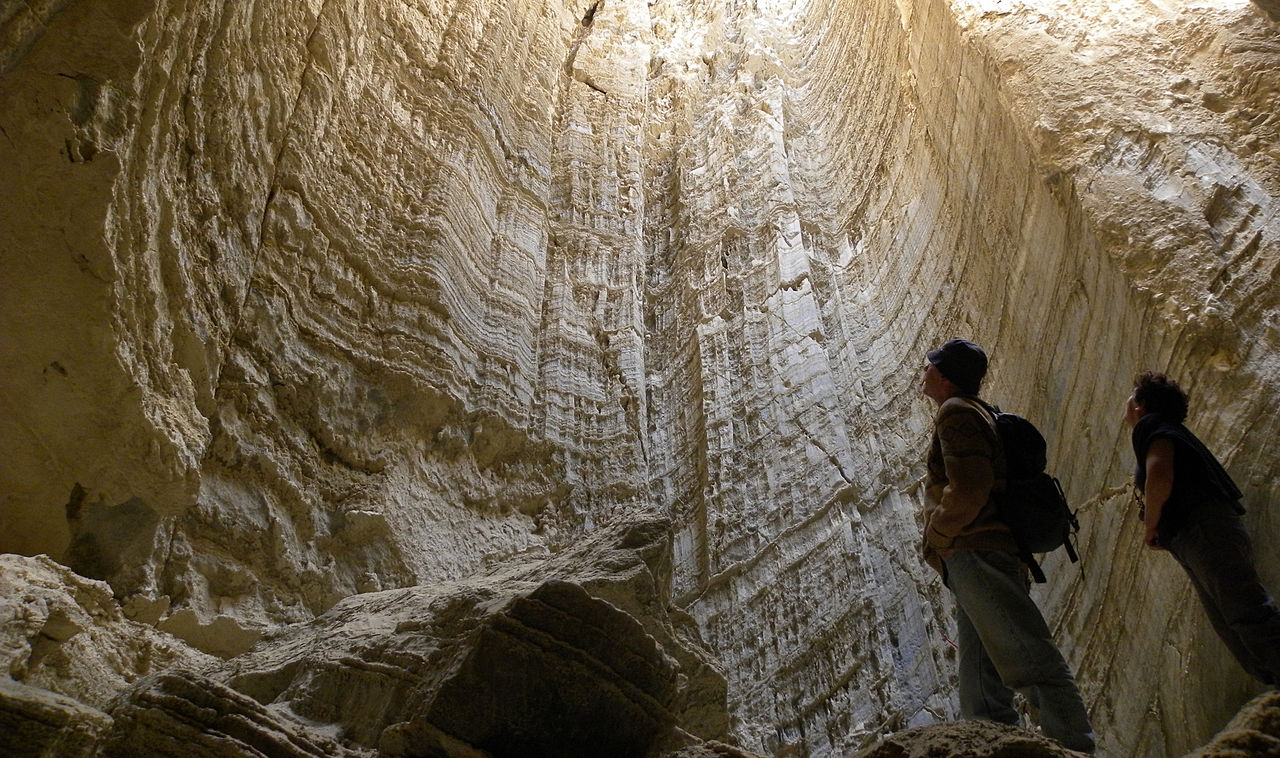
\includegraphics[height=2.8cm,width=1\textwidth,keepaspectratio]{surface_types/salt.jpg}\\
      \caption{Соляные отложения}
      \label{fig:surface_types/salt}
  \end{subfigure}
  \hfill
  \begin{subfigure}[b]{0.3\textwidth}
      \centering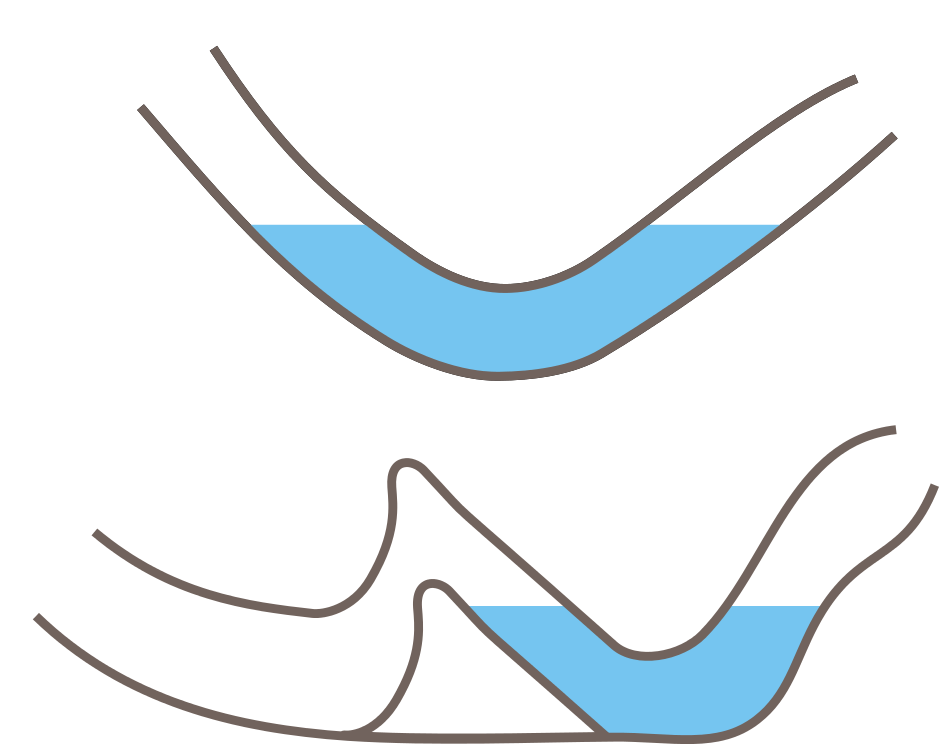
\includegraphics[height=2.8cm,width=1\textwidth,keepaspectratio]{surface_types/siphon.png}\\
      \caption{Сифон}
      \label{fig:surface_types/syphon}
  \end{subfigure}
  \hfill
  \begin{subfigure}[b]{0.3\textwidth}
      \centering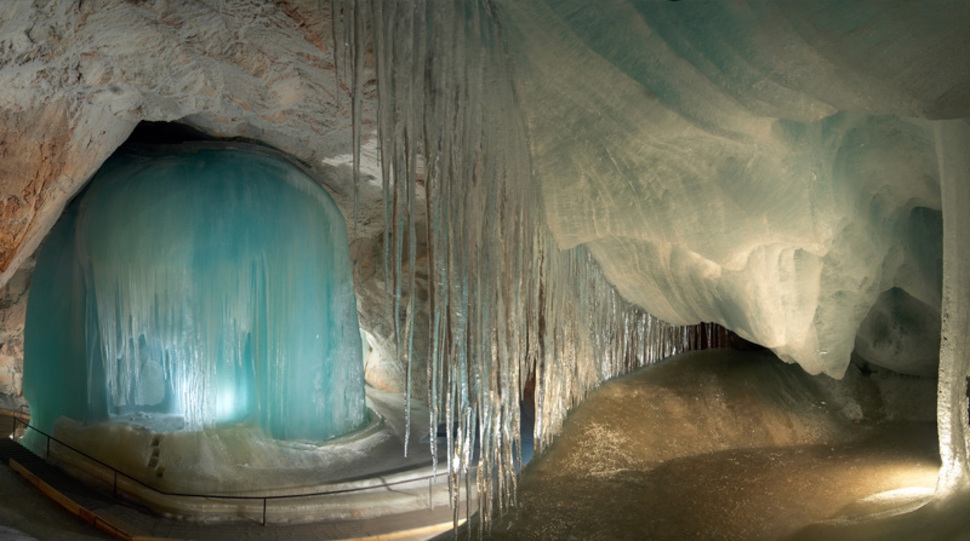
\includegraphics[height=2.8cm,width=1\textwidth,keepaspectratio]{surface_types/ice.png}\\
      \caption{Ледяная пещера}
      \label{fig:surface_types/ice}
  \end{subfigure}

  \begin{subfigure}[b]{0.3\textwidth}
      \centering
      \begin{tikzpicture}
          % Include the image in a node
          \node [above right, inner sep=0] (image) at (0,0)
          {\centering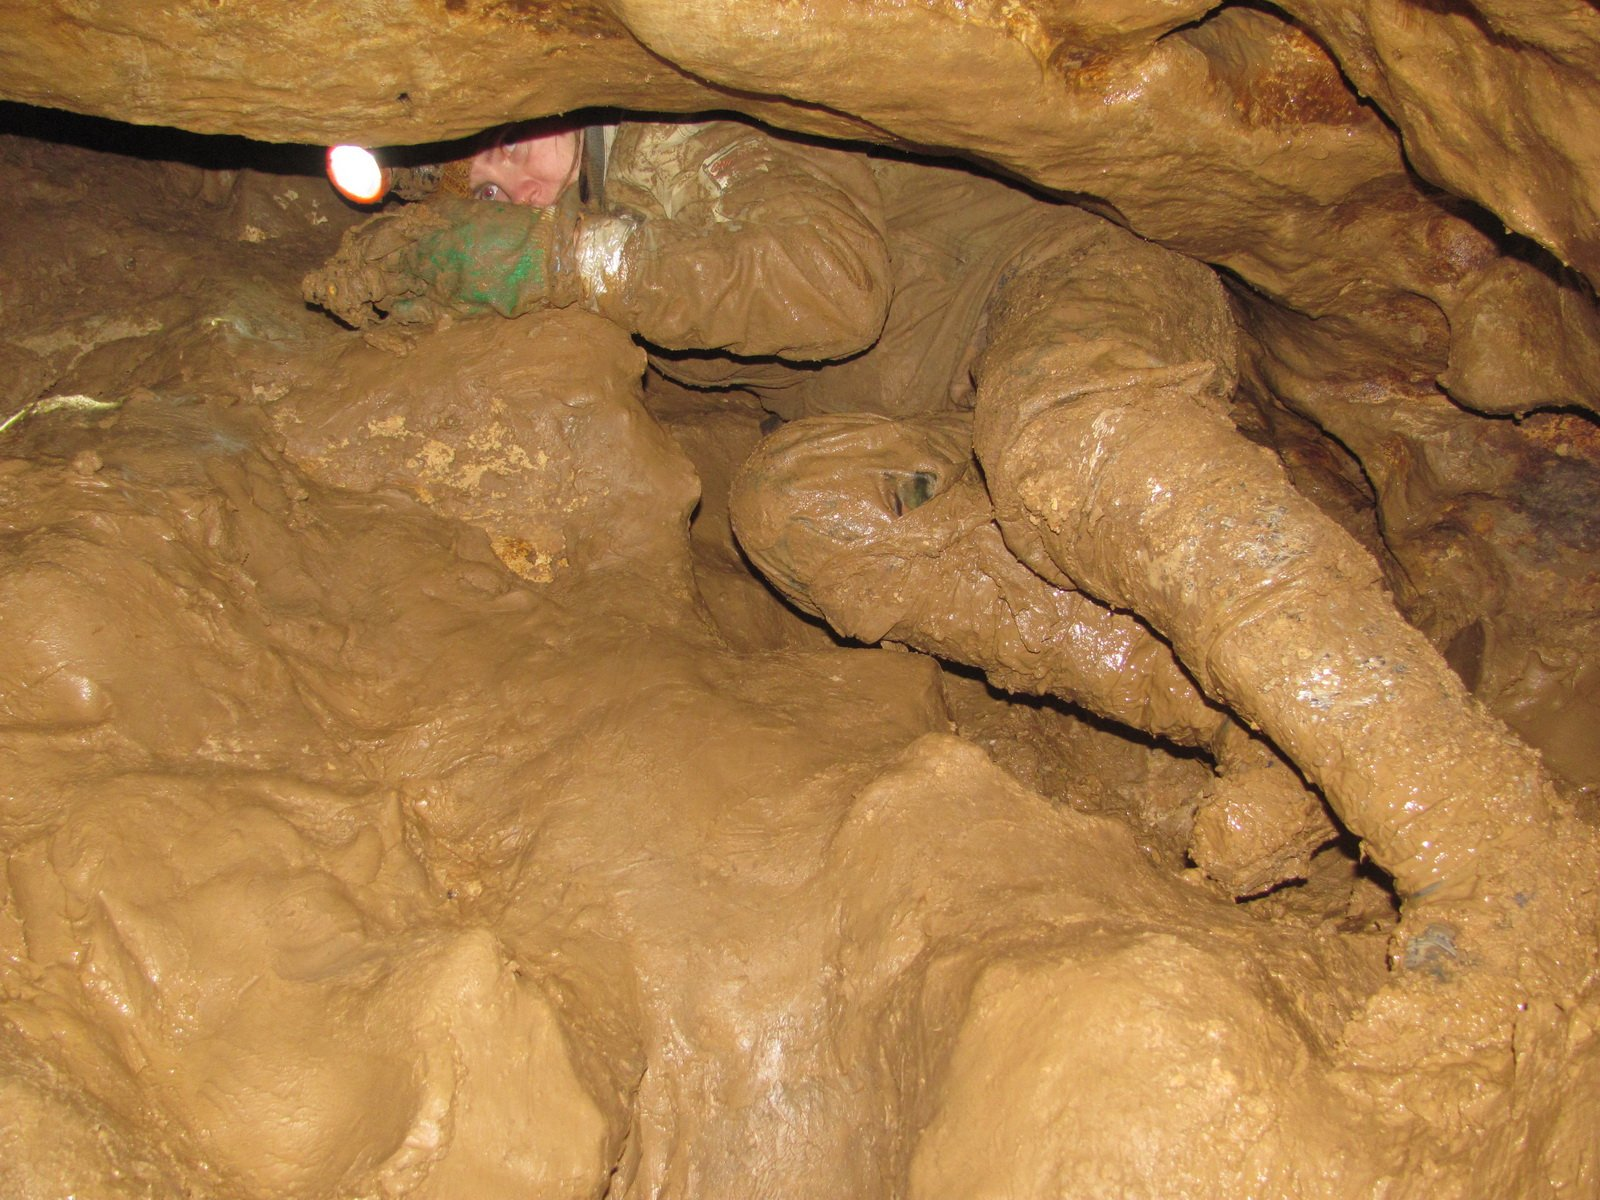
\includegraphics[height=2.8cm,width=1\textwidth,keepaspectratio]{surface_types/clay.jpg}};
          % Create scope with normalized axes
          \begin{scope}[
                  x={($ 0.1*(image.south east)$)},
                  y={($ 0.1*(image.north west)$)}]
              % Grid and axes' labels
              % \draw[lightgray,step=1] (image.south west) grid (image.north east);
              % \foreach \x in {0,1,...,10} { \node [below] at (\x,0) {\x}; }
              % \foreach \y in {0,1,...,10} { \node [left] at (0,\y) {\y};}
              % Labels
              \draw[stealth-, very thick,green] (6,8) -- ++(1,1)
              node[rounded corners=3pt,right,black,fill=white]{\tiny Человек};
          \end{scope}
      \end{tikzpicture}
      \caption{Глина}
      \label{fig:surface_types/clay}
  \end{subfigure}
  \hfill
  \begin{subfigure}[b]{0.3\textwidth}
      \centering
      \begin{tikzpicture}
          % Include the image in a node
          \node [above right, inner sep=0] (image) at (0,0)
          {\centering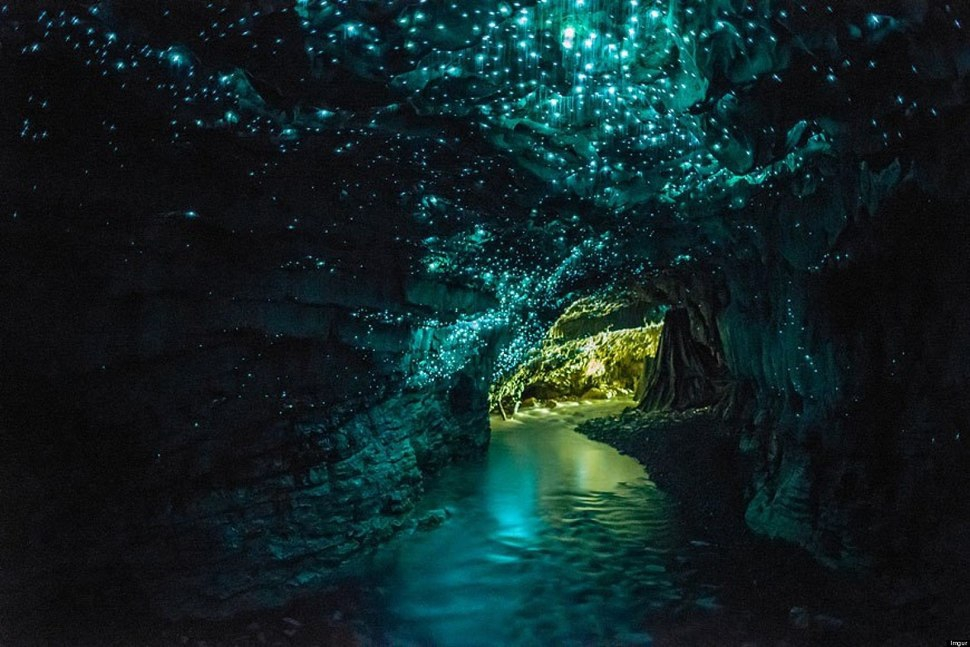
\includegraphics[height=2.8cm,width=1\textwidth,keepaspectratio]{surface_types/splash.png}};
          % Create scope with normalized axes
          \begin{scope}[
                  x={($ 0.1*(image.south east)$)},
                  y={($ 0.1*(image.north west)$)}]
              % Grid and axes' labels
              % \draw[lightgray,step=1] (image.south west) grid (image.north east);
              % \foreach \x in {0,1,...,10} { \node [below] at (\x,0) {\x}; }
              % \foreach \y in {0,1,...,10} { \node [left] at (0,\y) {\y};}

              % Labels
              \draw[stealth-, very thick,green] (5,2) -- ++(-2,+1)
              node[rounded corners=3pt,left,black,fill=white]{\tiny Лужа};
          \end{scope}
      \end{tikzpicture}
      \caption{Пещера, заполненная водой по~колено}
      \label{fig:surface_types/splash}
  \end{subfigure}
  \hfill
  \begin{subfigure}[b]{0.3\textwidth}
      \centering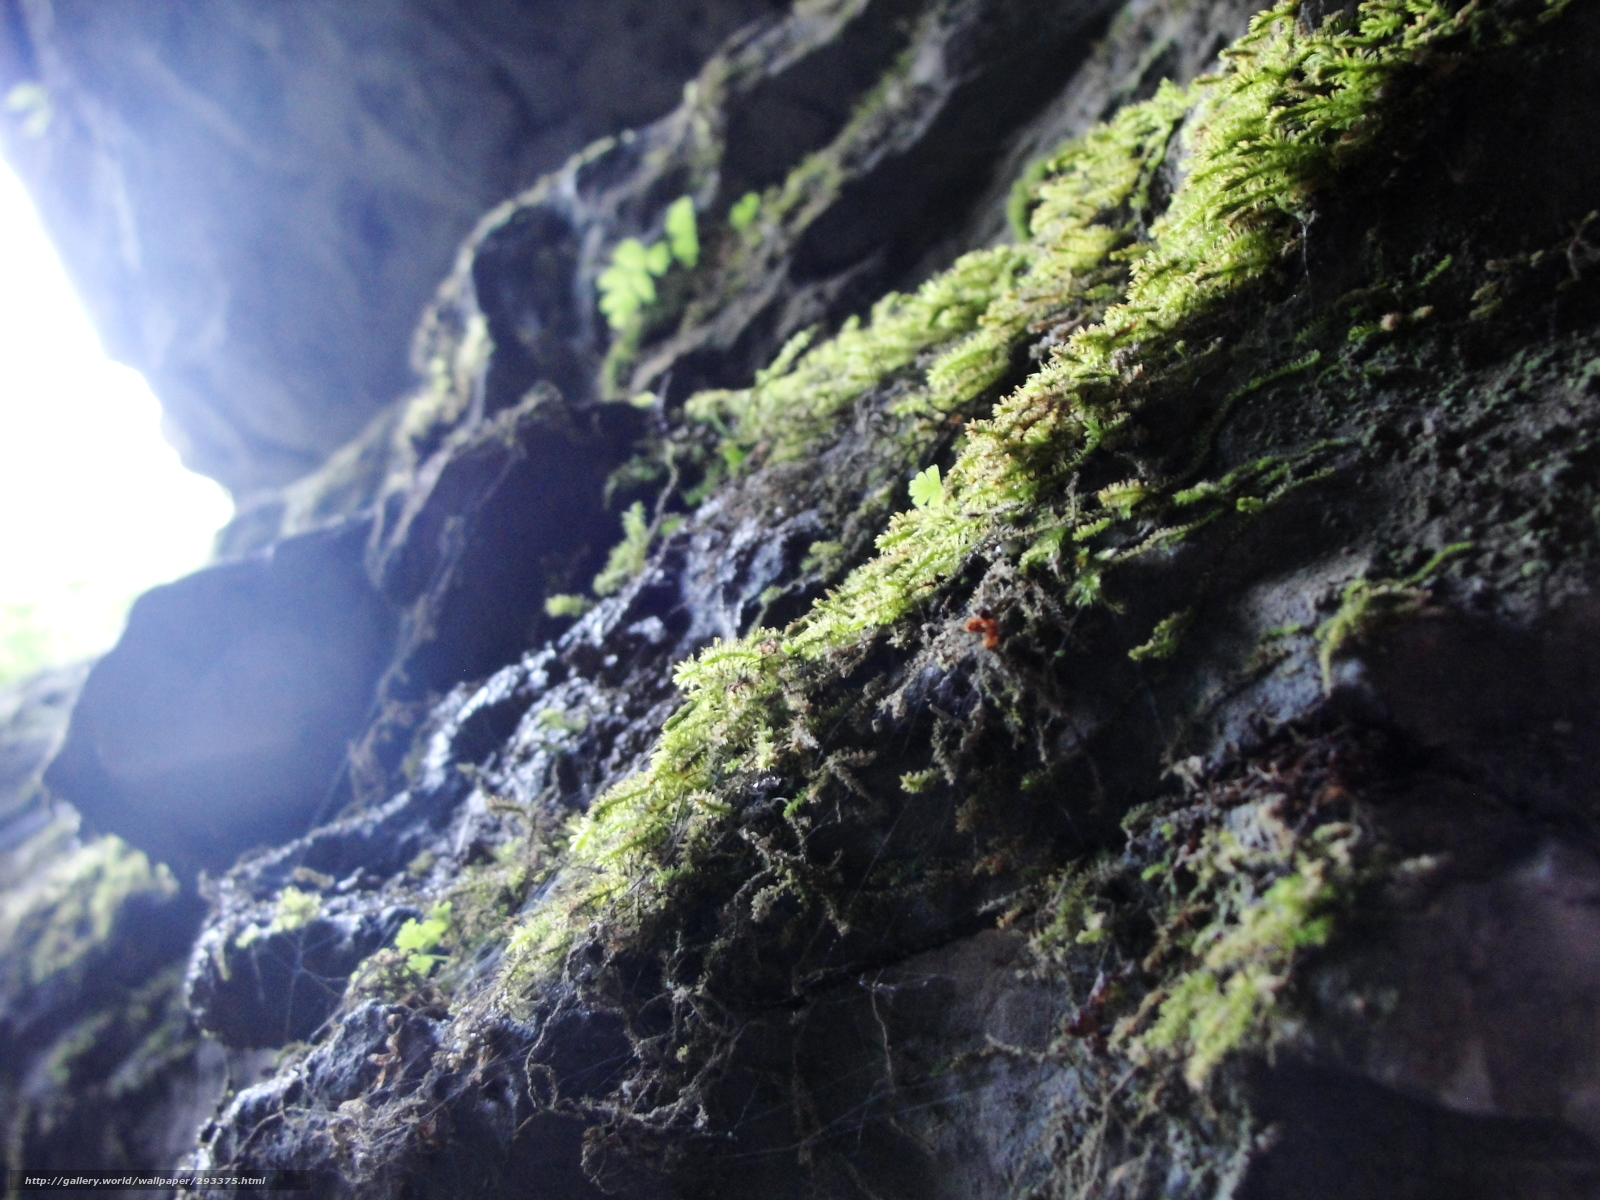
\includegraphics[height=2.8cm,width=1\textwidth,keepaspectratio]{surface_types/moss.jpg}\\
      \caption{Мох}
      \label{fig:surface_types/moss}
  \end{subfigure}
  \caption{Препятствия, встречающиеся в пещерах}\label{fig:obstacles}
\end{figure}


Эти препятствия могут встретиться человеком при исследовании или инспекции пещеры. Одно из преимуществ роботов --- они могут работать в опасных средах без нахождения рядом человека. Таким образом использование роботов в пещерах нивелирует все опасности для человека.

Существуют различные типы движителей роботов. С препятствиями представленными выше лучше всего справляются многоногие шагающие роботы. Такие роботы могут проходить по сыпучим грунтам, каменистым грядам и преодолевать небольшие водные преграды.

Для полноценного функционирования в пещере необходимы сенсоры. Внешними сенсорами являются камера и лидар.

Характерные для пещеры условия могут вывевсти из строя сенсоры. К примеру грязь \pic{fig:surface_types/clay} может закрыть обзор камере или лидару. Или водная гладь \pic{fig:surface_types/splash} будет отражать лучи лазера лидара и искажать данные \pic{fig:unsolvable_case}.

      \begin{figure}[h]
      \begin{subfigure}[t]{0.3\textwidth}
        \centering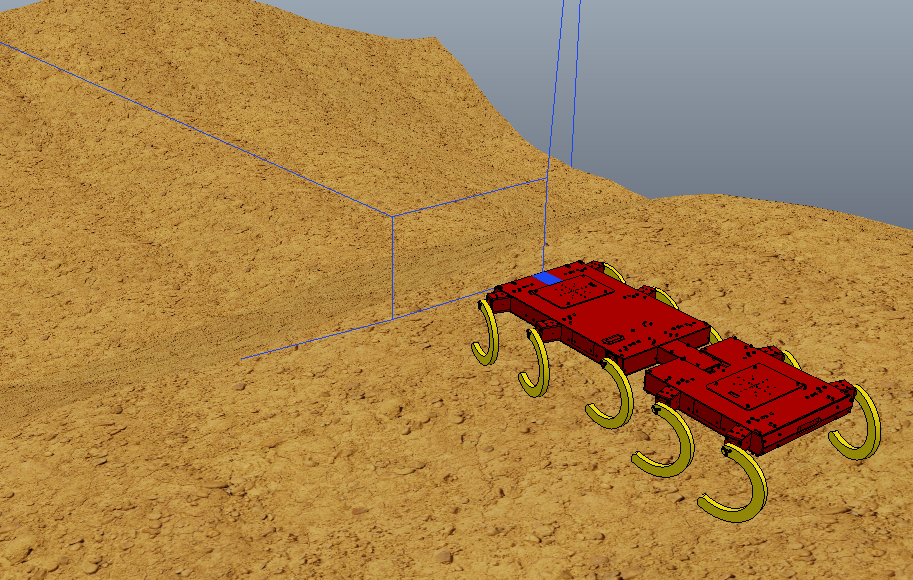
\includegraphics[height=3cm,width=1\textwidth,keepaspectratio]{terrain_wo_water.png}
        \caption{Территория без воды}
    \end{subfigure}
          \begin{subfigure}[t]{0.35\textwidth}
              \centering
              \begin{tikzpicture}
                  % Include the image in a node
                  \node [above right, inner sep=0] (image) at (0,0)
                  {\centering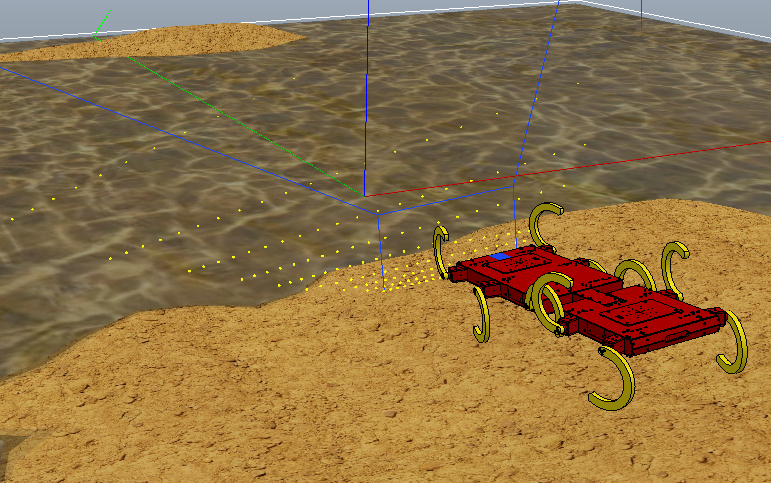
\includegraphics[height=3.5cm,width=1\textwidth,keepaspectratio]{terrain_w_water1.png}};
                  % Create scope with normalized axes
                  \begin{scope}[
                          x={($ 0.1*(image.south east)$)},
                          y={($ 0.1*(image.north west)$)}]
                      % Grid and axes' labels
                      \draw[stealth-, very thick,green] (6,8) -- ++(2,1)
                      node[rounded corners=3pt,right,black,fill=white]{\tiny Вода};

                      \draw[stealth-, very thick,green] (0.5,5.5) -- (3,2);
                      \draw[stealth-, very thick,green] (2.5,4.2) -- (3,2);
                      \draw[stealth-, very thick,green] (4.5,4) -- (3,2)
                      node[rounded corners=3pt,below,black,fill=white]{\tiny Данные с лидара};
                  \end{scope}
              \end{tikzpicture}
              \caption{Территория с водой}
              \label{fig:terrain_w_water1.png}
          \end{subfigure}
          \begin{subfigure}[t]{0.3\textwidth}
              \centering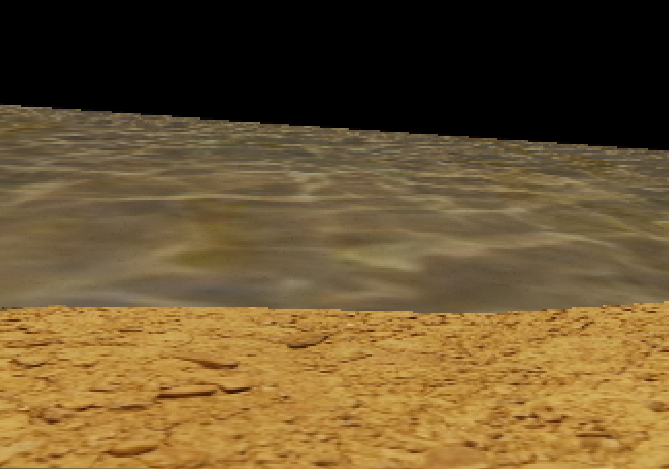
\includegraphics[height=3cm,width=1\textwidth,keepaspectratio]{terrain_w_water_camera.png}
              \caption{Изображение с камеры}
          \end{subfigure}
          \caption{Пример ситуации, где навигация, основанная на камере или лидаре построит неправильную карту}
          \label{fig:unsolvable_case}
      \end{figure}
  % \legend{Подрисуночный текст, описывающий обозначения, например. Согласно
  %     ГОСТ 2.105, пункт 4.3.1, располагается перед наименованием рисунка.}

% \ifsynopsis
% Этот абзац появляется только в~автореферате.
% Для формирования блоков, которые будут обрабатываться только в~автореферате,
% заведена проверка условия \verb!\!\verb!ifsynopsis!.
% Значение условия задаётся в~основном файле документа (\verb!synopsis.tex! для
% автореферата).
% \else
% Этот абзац появляется только в~диссертации.
% Через проверку условия \verb!\!\verb!ifsynopsis!, задаваемого в~основном файле
% документа (\verb!dissertation.tex! для диссертации), можно сделать новую
% команду, обеспечивающую появление цитаты в~диссертации, но~не~в~автореферате.
% \fi

{\aim} работы является разработка и исследование робототехнической системы построения карты местности и определения геометрических и физических свойств опорной поверхности на базе многоногого шагающего аппарата с тактильным очувствлением без использования оптических сенсоров.

Данное решение отлично подходит для первичного исследования замкнутых труднодоступных пространств, где отсутствует освещение, обилие грязи, пыли, а так же водных препятствий. Алгоритмы и концепты навигации данной системы могут быть использованы как резервная система навигации для других робототехнических систем, когда более точная --- оптическая вышла из строя.

Для~достижения поставленной цели решаются следующие {\tasks}:
\begin{enumerate}[beginpenalty=10000] % https://tex.stackexchange.com/a/476052/104425
    \item разрабатока метода оптимизации конструкции многоногих шагающих роботов с цикловыми движителями с одной степенью свободы по критериям проходимости (длина робота), детализации (количества ног), пройденного пути;
    \item создание методики исследования датчика силы, когда площадь контакта нажатия на сенсор меньше чувствительной области самого сенсора;
  \item  проектирование метода построения карты местности и определения поверхности с помощью тактильного очувствления;
  \item реализация алгоритма, позволяющего определять геометрические и физические свойства опорной поверхности.
\end{enumerate}

{\researchobj}
Объектом исследования является класс многоногих шагающих роботов с цельным или сочленённым корпусом, и цикловыми движителями с одной степенью свободы, управляемые зависимо или независимо друг от друга.

\begin{figure}[H]
  \centering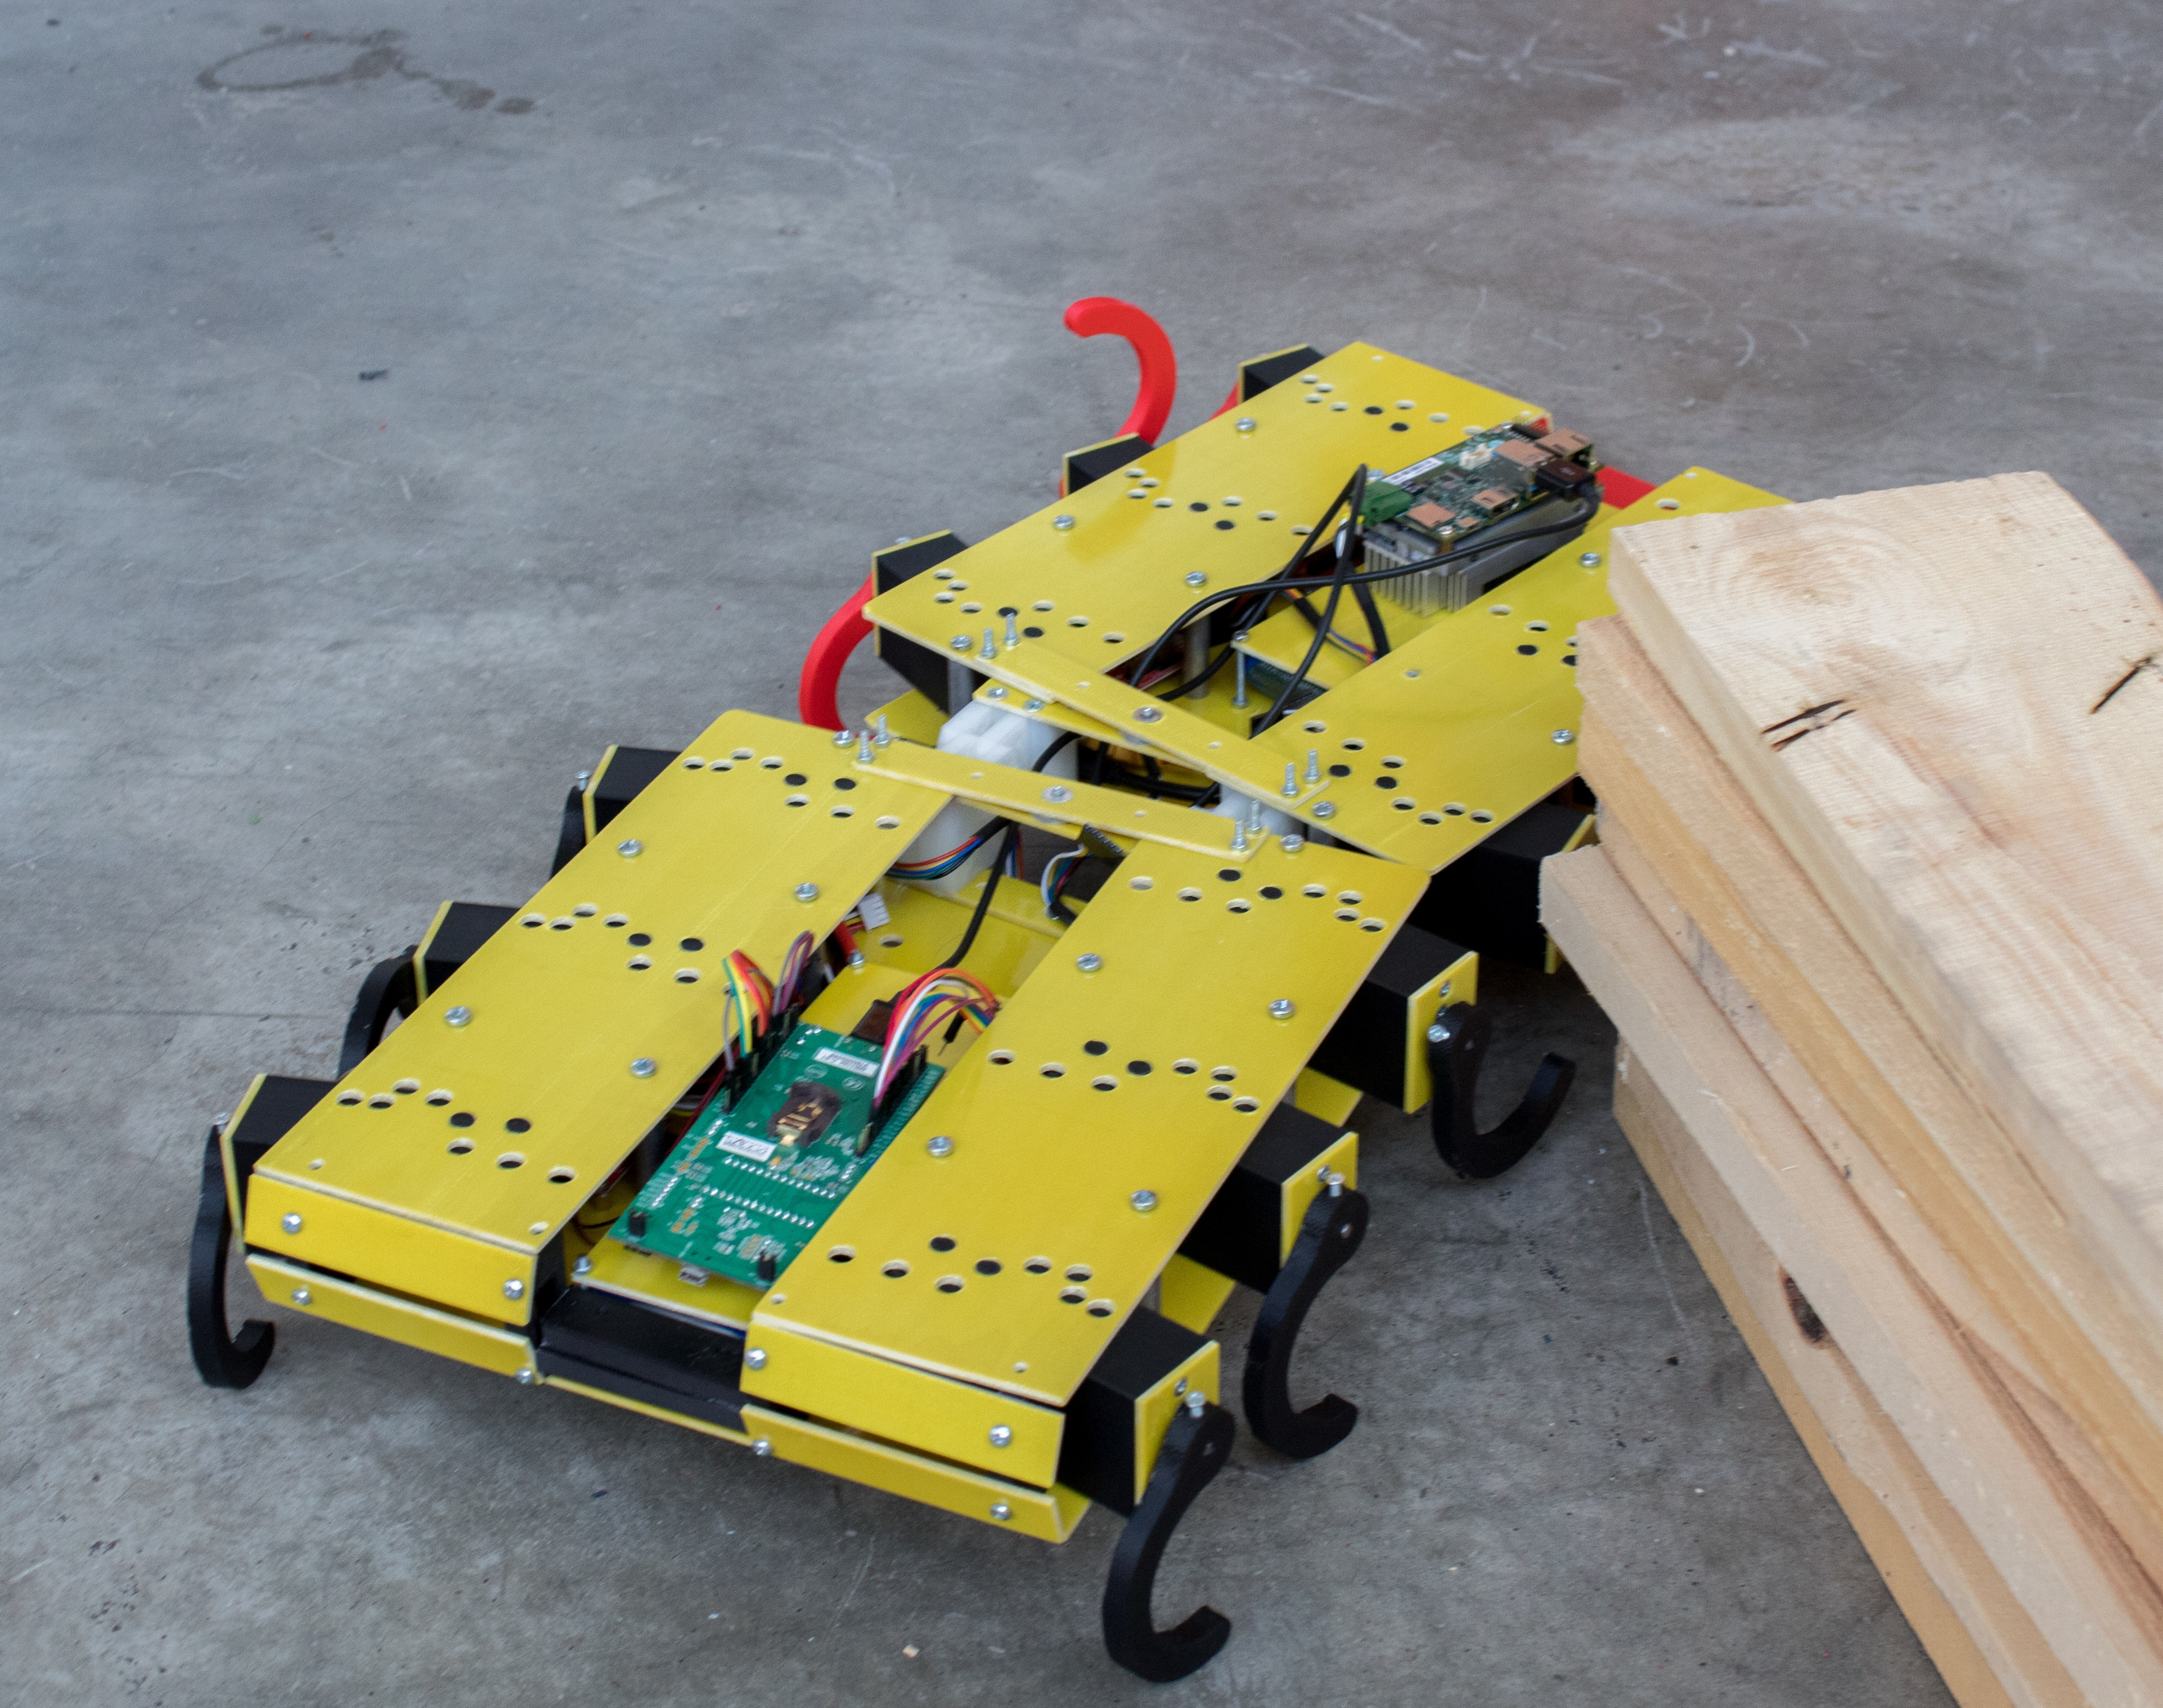
\includegraphics[height=7cm,width=1\textwidth,keepaspectratio]{strirus_2.jpg}
  \caption{Прототип, на котором было сделано большинство экспериментов}
  \label{fig:strirus_2.jpgg}
\end{figure}

Основная часть экспериментальных исследований проведена с прототипом \pic{fig:strirus_2.jpgg}, корпус которого состоит из двух сегментов с одной активной степенью свободы. Робот обладает 12 независимыми педипуляторами, 6 ног в первом сегменте и 6 во втором.

Особенность конструкции робота в том, что возможно изменять угол между ногой и корпусом робота. Данное конструктивное изменение позволило сделать перемещение робота всенаправленным, то есть робот может двигаться во все стороны без смены ориентации корпуса робота.


{\methods} За основу были взяты методологии из теории по разработке робототехнических систем, теоретической механики, механизмов и машин, теории оптимизации.

Для экспериментального исследования применялось численное и стендовое моделирования.

{\reliability} Правдивость результатов обеспечивается согласованностью с опубликованными результатами научных исследований других авторов, подтверждаются результатами компьютерного моделирования, натурными испытаниями. Результаты диссертационного исследования докладывались и обсуждались на российских и международных научных конференциях, и получили положительный отзыв научной общественности.


{\novelty} Сформулирована и решена задача построения карты местности с помощью тактильного очувствления шагающего робота с цикловыми движителями и датчиками силы, установленными на опорных поверхностях движителей.
Разработан метод оптимизации конструкции многоногого шагающего робота с цикловыми движителями. 
Разработана методика автоматизированного исследования датчика силы.


\textbf{Доказана} возможность построения карты местности и определения типа поверхности с помощью тактильного очувствления как в робототехническом симуляторе, так с помощью натурного эксперимента.

\textbf{Показано}, что оптимальное количество ног для циклового движителя с одной степенью свободы в ноге находится в диапазоне от 8 до 14 ног. 

\textbf{Предложено} использовать преобразователь силы на основе полимерного материала Velostat. \textbf{Установлено}, что данный преобразователь можно использовать для изначальной задачи, то есть при площади контакта с поверхностью большей, чем 25\% площади сенсора. 

\textbf{Сделан вывод} об эффективности предложенных методик, на основе результатов натурных испытаний.

{\defpositions}
\begin{enumerate}[beginpenalty=10000] % https://tex.stackexchange.com/a/476052/104425
  \item метод оптимизации конструкции многоногих шагающих роботов с цикловыми движителями с одной степенью свободы по критериям проходимости (длина робота), детализации (количества ног), пройденного пути;
  \item метод исследования датчика силы, когда площадь соприкосновения меньше площади сенсора;
  \item алгоритм, позволяющий определять тип поверхности;
  \item метод построения карты местности с помощью датчиков силы, установленных на ногах робота.
\end{enumerate}


{\influence} Реализация полученных результатов в виде продукта позволит получать информацию о типе пройденной поверхности, а так же строить карту поверхности под небольшим слоем воды (лужа), там где лидар и камера не смогут выдать адекватный результат.


{\probation}
Основные результаты работы докладывались~на:
\begin{itemize}
  \item ICINCO 2017 --- 14th International Conference on Informatics in Control, Automation and Robotics (Madrid, Spain, 26-28 july 2017);
  \item IEEE International Conference on Robotics and Biomimetics, ROBIO 2017 (Macau, China, 5-8 december 2017);
  \item  международной  научно-практической  конференции  «Прогресс  транспортных 
  средств и систем» (г. Волгоград, 9-11 октября 2018 г.);
  \item 23rd IEEE FRUCT Conference (Bologna, Italy, 13-16 november 2018).
  \item XXXI международной конференции молодых ученых и студентов МИКМУС-2019 
  (г. Москва, 4-6 декабря 2019 г.);
  \item Международная конференция <<Зимняя Школа Робототехники в Сириусе --- 2022>> (г. Адлер, Россия, 25 января - 6 февраля 2022)
\end{itemize}

{\contribution} Все научные результаты диссертации, выдвигаемые для защиты, получены автором лично.

% Вставка кто сколько опубликовался
\ifsynopsis
\ifnumequal{\value{bibliosel}}{0}
{%%% Встроенная реализация с загрузкой файла через движок bibtex8. (При желании, внутри можно использовать обычные ссылки, наподобие `\cite{vakbib1,vakbib2}`).
    {\publications} Основные результаты по теме диссертации изложены
    в~XX~печатных изданиях,
    X из которых изданы в журналах, рекомендованных ВАК,
    X "--- в тезисах докладов.
}%
{%%% Реализация пакетом biblatex через движок biber
    \begin{refsection}[bl-author, bl-registered]
        % Это refsection=1.
        % Процитированные здесь работы:
        %  * подсчитываются, для автоматического составления фразы "Основные результаты ..."
        %  * попадают в авторскую библиографию, при usefootcite==0 и стиле `\insertbiblioauthor` или `\insertbiblioauthorgrouped`
        %  * нумеруются там в зависимости от порядка команд `\printbibliography` в этом разделе.
        %  * при использовании `\insertbiblioauthorgrouped`, порядок команд `\printbibliography` в нём должен быть тем же (см. biblio/biblatex.tex)
        %
        % Невидимый библиографический список для подсчёта количества публикаций:
        \printbibliography[heading=nobibheading, section=1, env=countauthorvak,          keyword=biblioauthorvak]%
        \printbibliography[heading=nobibheading, section=1, env=countauthorwos,          keyword=biblioauthorwos]%
        \printbibliography[heading=nobibheading, section=1, env=countauthorscopus,       keyword=biblioauthorscopus]%
        \printbibliography[heading=nobibheading, section=1, env=countauthorconf,         keyword=biblioauthorconf]%
        \printbibliography[heading=nobibheading, section=1, env=countauthorother,        keyword=biblioauthorother]%
        \printbibliography[heading=nobibheading, section=1, env=countregistered,         keyword=biblioregistered]%
        \printbibliography[heading=nobibheading, section=1, env=countauthorpatent,       keyword=biblioauthorpatent]%
        \printbibliography[heading=nobibheading, section=1, env=countauthorprogram,      keyword=biblioauthorprogram]%
        \printbibliography[heading=nobibheading, section=1, env=countauthor,             keyword=biblioauthor]%
        \printbibliography[heading=nobibheading, section=1, env=countauthorvakscopuswos, filter=vakscopuswos]%
        \printbibliography[heading=nobibheading, section=1, env=countauthorscopuswos,    filter=scopuswos]%
        %
        \nocite{*}%
        %
        {\publications} Основные результаты по теме диссертации изложены в~\arabic{citeauthor}~печатных изданиях,
        \arabic{citeauthorvak} из которых изданы в журналах, рекомендованных ВАК\sloppy%
        \ifnum \value{citeauthorscopuswos}>0%
            , \arabic{citeauthorscopuswos} "--- в~периодических научных журналах, индексируемых Web of~Science и Scopus\sloppy%
        \fi%
        \ifnum \value{citeauthorconf}>0%
            , \arabic{citeauthorconf} "--- в~тезисах докладов.
        \else%
            .
        \fi%
        \ifnum \value{citeregistered}=1%
            \ifnum \value{citeauthorpatent}=1%
                Зарегистрирован \arabic{citeauthorpatent} патент.
            \fi%
            \ifnum \value{citeauthorprogram}=1%
                Зарегистрирована \arabic{citeauthorprogram} программа для ЭВМ.
            \fi%
        \fi%
        \ifnum \value{citeregistered}>1%
            Зарегистрированы\ %
            \ifnum \value{citeauthorpatent}>0%
            \formbytotal{citeauthorpatent}{патент}{}{а}{}\sloppy%
            \ifnum \value{citeauthorprogram}=0 . \else \ и~\fi%
            \fi%
            \ifnum \value{citeauthorprogram}>0%
            \formbytotal{citeauthorprogram}{программ}{а}{ы}{} для ЭВМ.
            \fi%
        \fi%
        % К публикациям, в которых излагаются основные научные результаты диссертации на соискание учёной
        % степени, в рецензируемых изданиях приравниваются патенты на изобретения, патенты (свидетельства) на
        % полезную модель, патенты на промышленный образец, патенты на селекционные достижения, свидетельства
        % на программу для электронных вычислительных машин, базу данных, топологию интегральных микросхем,
        % зарегистрированные в установленном порядке.(в ред. Постановления Правительства РФ от 21.04.2016 N 335)
    \end{refsection}%
    \begin{refsection}[bl-author, bl-registered]
        % Это refsection=2.
        % Процитированные здесь работы:
        %  * попадают в авторскую библиографию, при usefootcite==0 и стиле `\insertbiblioauthorimportant`.
        %  * ни на что не влияют в противном случае
        \nocite{vakbib2}%vak
        \nocite{patbib1}%patent
        \nocite{progbib1}%program
        \nocite{bib1}%other
        \nocite{confbib1}%conf
    \end{refsection}%
        %
        % Всё, что вне этих двух refsection, это refsection=0,
        %  * для диссертации - это нормальные ссылки, попадающие в обычную библиографию
        %  * для автореферата:
        %     * при usefootcite==0, ссылка корректно сработает только для источника из `external.bib`. Для своих работ --- напечатает "[0]" (и даже Warning не вылезет).
        %     * при usefootcite==1, ссылка сработает нормально. В авторской библиографии будут только процитированные в refsection=0 работы.
}
% При использовании пакета \verb!biblatex! будут подсчитаны все работы, добавленные
% в файл \verb!biblio/author.bib!. Для правильного подсчёта работ в~различных
% системах цитирования требуется использовать поля:
% \begin{itemize}
%         \item \texttt{authorvak} если публикация индексирована ВАК,
%         \item \texttt{authorscopus} если публикация индексирована Scopus,
%         \item \texttt{authorwos} если публикация индексирована Web of Science,
%         \item \texttt{authorconf} для докладов конференций,
%         \item \texttt{authorpatent} для патентов,
%         \item \texttt{authorprogram} для зарегистрированных программ для ЭВМ,
%         \item \texttt{authorother} для других публикаций.
% \end{itemize}
% Для подсчёта используются счётчики:
% \begin{itemize}
%         \item \texttt{citeauthorvak} для работ, индексируемых ВАК,
%         \item \texttt{citeauthorscopus} для работ, индексируемых Scopus,
%         \item \texttt{citeauthorwos} для работ, индексируемых Web of Science,
%         \item \texttt{citeauthorvakscopuswos} для работ, индексируемых одной из трёх баз,
%         \item \texttt{citeauthorscopuswos} для работ, индексируемых Scopus или Web of~Science,
%         \item \texttt{citeauthorconf} для докладов на конференциях,
%         \item \texttt{citeauthorother} для остальных работ,
%         \item \texttt{citeauthorpatent} для патентов,
%         \item \texttt{citeauthorprogram} для зарегистрированных программ для ЭВМ,
%         \item \texttt{citeauthor} для суммарного количества работ.
% \end{itemize}
% % Счётчик \texttt{citeexternal} используется для подсчёта процитированных публикаций;
% % \texttt{citeregistered} "--- для подсчёта суммарного количества патентов и программ для ЭВМ.

% Для добавления в список публикаций автора работ, которые не были процитированы в
% автореферате, требуется их~перечислить с использованием команды \verb!\nocite! в
% \verb!Synopsis/content.tex!.

\fi

Диссертационная работа была выполнена при поддержке грантов:
\begin{itemize}
    \item НТИ по поддержке Центра <<Технологий Компонентов Робототехники и Мехатроники>> на базе Университета Иннополис по теме <<Разработка роботизированных платформ для автономной подземной и наземной инспекции местности в условиях трудной проходимости и плохой видимости>>. 
    \item РФФИ № 20-38-90265 по теме <<Разработка метода очувствления мобильного шагающего робота, перемещающегося в закрытом пространстве естественного происхождения>>.
\end{itemize}

{\struct}


% В введении рассказывается об актуальности проблемы, в чем научная новизна и цель проекта. Во первой главе показан обзор существующих решений. Вторая глава покрывает разработку объекта исследования, а именно решение задачи топологического синтеза и инженерную разработку прототипа. Третья глава посвящена разработке и исследованию самодельного преобразователя силы на основе Velostat. Четвертая глава раскрывает детали создания алгоритма построения карты с помощью тактильного очувствления, определения типа поверхности.
% Четвертая глава раскрывает детали создания алгоритма построения карты с помощью тактильного очувствления, решение проблемы локализации с помощью датчиков датчиков силы, IMU и маяков. Решатся проблема определения типа поверхности. % Характеристика работы по структуре во введении и в автореферате не отличается (ГОСТ Р 7.0.11, пункты 5.3.1 и 9.2.1), потому её загружаем из одного и того же внешнего файла, предварительно задав форму выделения некоторым параметрам

{\struct} Диссертация состоит из~введения,
\formbytotal{totalchapter}{глав}{ы}{}{},
заключения и
\formbytotal{totalappendix}{приложен}{ия}{ий}{}.
%% на случай ошибок оставляю исходный кусок на месте, закомментированным
%Полный объём диссертации составляет  \ref*{TotPages}~страницу
%с~\totalfigures{}~рисунками и~\totaltables{}~таблицами. Список литературы
%содержит \total{citenum}~наименований.
%
Полный объём диссертации составляет
\formbytotal{TotPages}{страниц}{у}{ы}{}, включая
\formbytotal{totalcount@figure}{рисун}{ок}{ка}{ков} и
\formbytotal{totalcount@table}{таблиц}{у}{ы}{}.
Список литературы содержит
\formbytotal{citenum}{наименован}{ие}{ия}{ий}.
    % Введение
\ifnumequal{\value{contnumfig}}{1}{\counterwithout{figure}{chapter}
}{\counterwithin{figure}{chapter}}
\ifnumequal{\value{contnumtab}}{1}{\counterwithout{table}{chapter}
}{\counterwithin{table}{chapter}}
\chapter{Обзор и анализ робототехнических систем, условия их применения}\label{ch:ch1}
Так как целью работы является разработка и исследование робототехнической системы, то первым щагом является рассмотрение других систем, которые используются в найденных местах. Критичным является понимание причин использования конкретных движителей в системах, их плюсов и минусов. Необходимо классифицировать существующие типы движитилей, понять куда встраивается текущий коцнепт. Сравнить его с остальными роботами из его семейства. Все это поможет избежать типичные проблемы, связанные с конкретым типом движителя, которые неочевидны по началу разработки.

\section{Классификация машин, использующих ноги в качестве движителя}
Эта классификация основана на работе \cite{Maloletov2015dinamica}. Первые попытки создания многоногих роботов были предприняты в эпоху до нашей эры. В настоящее время можно найти десятки конструкций шагающих роботов, но, как правило, это только экспериментальные прототипы. Следовательно, классифицировать их --- задача не из легких. Более того, смысл <<ходьбы>> не так очевиден, и некоторые исследователи трактуют его по-другому \cite{Bel1984,Brisk2009,Ohom1984,Pavl2013}. 

Определяющей особенностью аппарата, которая в целом позволяет говорить о шагании, является наличие специальных механизмов (ног, шагающих механизмов), которые обеспечивают движение аппарата в результате дискретного взаимодействия с опорой. Под дискретным взаимодействием понимают ситуацию, когда есть моменты времени, в которые механизм контактирует с опорной площадкой, и моменты времени, в которые с опорой механизм не взаимодействует.

Существует несколько видов локомоции. Один из них - ходьба. Обычно это тип передвижения, когда за один раз одна нога касается опоры. Если возникает ситуация, когда ни одна нога не касается земли, это можно назвать прыжком или бегом \cite{Ohom1984}. Если фаза движения машины с опорой на ноги чередуется с фазой покоя, в которой машина неподвижно лежит на опорной поверхности, то такое движение называется ползанием. Ходьба, прыжки, трусца, бег и ползание предполагают, что соединение ног с опорной поверхностью является неретенционным. Однако ноги могут быть оснащены специальными устройствами - захватами, присосками и т.п., позволяющими устройству осуществлять удерживающие связи с опорной поверхностью. Тип движения такого устройства называется лазанием.

Подводя итог, можно сказать, что классификация следующая. Важно отметить, что в одном экземпляре может сочетаться несколько типов движителей.
\begin{enumerate}
\item Псевдо-шагание
\item Шагающие машины с дополнительными опорными механизмами
\item Шагающие машины с движителями циклического действия
\item Ходьба с импровизированным следом
\begin{enumerate}
\item Ходьба - колесная
\item Прыжки и бег
\item Ползание
\item Лазание
\end{enumerate}
\end{enumerate}

Псевдошагающие машины похожи на роботов с ногами, но их ноги всегда касаются земли. Другими словами, эти машины могут только имитировать движение. Одним из распространенных примеров является игрушка, называемая шагающий слон \pic{fig:mechEleph}.


\begin{figure}[H]
\centering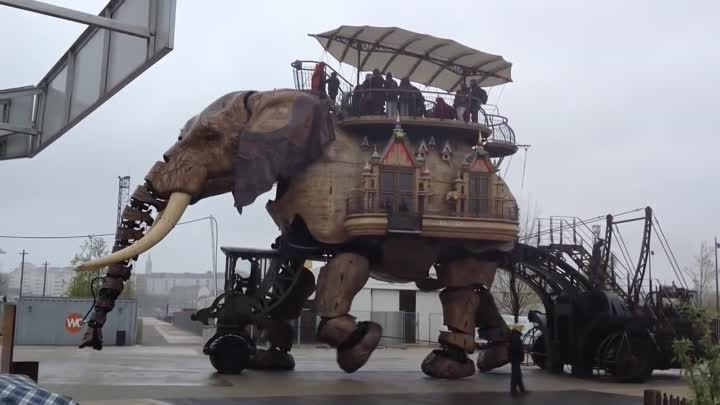
\includegraphics[width=0.8\textwidth]{from_master/mechEleph}
\caption{Механический слон}
\label{fig:mechEleph}
\end{figure}

К классу шагающих машин с дополнительными опорами относятся устройства, имеющие помимо дискретно взаимодействующих с опорной поверхностью шагающих движителей дополнительные механизмы, постоянно контактирующие с опорой. Необходимость в дополнительных опорах обычно возникает тогда, когда шагающих движителей недостаточно для обеспечения устойчивости машины. Чаще всего для этой цели шагающее транспортное средство оснащается колесной тележкой (рис. \ref{fig:Riksha},\ref{fig:steamMan})\cite{Brisk2011, Petr1986}.

\begin{figure}[H]
\centering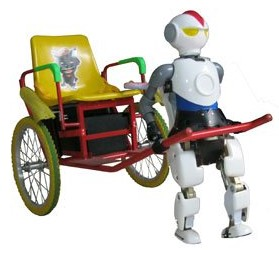
\includegraphics[width=0.6\textwidth]{from_master/Riksha}
\caption{Riksha type robot}
\label{fig:Riksha}
\end{figure}

\begin{figure}[H]
\centering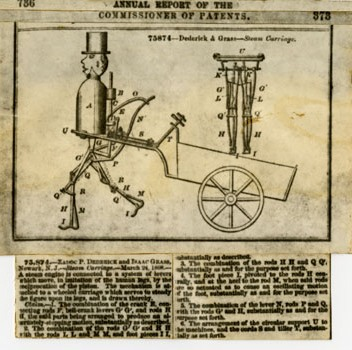
\includegraphics[width=0.6\textwidth]{from_master/steamMan}
\caption{Робот паровой человек}
\label{fig:steamMan}
\end{figure}

Обычно такие машины используются для демонстрации или для отладки системы управления. Использовать их на практике бессмысленно, так как они не имеют никаких преимуществ по сравнению с колесными роботами.


\subsection{Шагающие машины с циклическими движителями}
Этот тип имеет несколько особенностей. Он характеризуется тем, что опорные точки шагающих механизмов движутся по одной и той же траектории относительно корпуса машины, и не решают проблемы адаптации к грунту и выбора точек постановки ног на землю. Такие машины имеют лучшую проходимость по сравнению с колесами меньшее сопротивление движению от земли, лучшее сцепление с основной поверхностью, большие возможности для снижения давления на грунт \cite{cruse2001control}. Примеры машин с циклическими движителями: (рис. \ref{fig:chebishev},\ref{fig:kuban}).

\begin{figure}[H]
\centering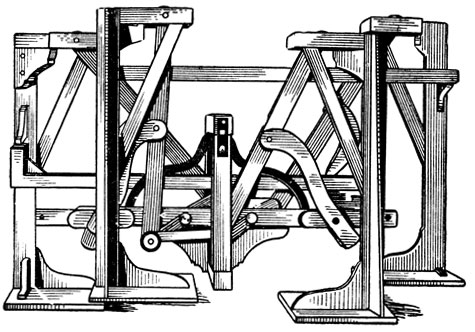
\includegraphics[width=0.7\textwidth]{from_master/chebishev}
\caption{Машина Чебышева}
\label{fig:chebishev}
\end{figure}

\begin{figure}[H]
\centering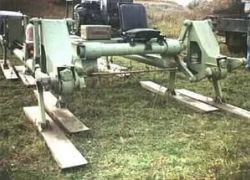
\includegraphics[width=0.7\textwidth]{from_master/kuban.jpg}
\caption{Робот ВолгГТУ Кубань}
\label{fig:kuban}
\end{figure}

Главным преимуществом машин с циклическим шагающим движителем по сравнению с другими шагающими машинами является простота их конструкции и управления.

Ходьба с импровизированным следом модификация предыдущего типа движителя и она дает наибольшие преимущества по сравнению с другими заявленными типами движителей. 

Он может принимать постановку ноги на землю, произвольный закон изменения скорости движения ноги как на этапе взаимодействия с землей, так и на этапе переноса. Такие машины значительно превосходят традиционные транспортные средства не только по грунту, но и по профильной проходимости. А их главным недостатком является сложность конструкции и системы управления. Это самый многочисленный и разнообразный класс шагающих машин, и большинство приведенных ниже примеров, за исключением специально оговоренных случаев, относятся именно к нему.

Колесно-шагающими машинами традиционно называют класс устройств, в которых колеса шагающих движителей служат упорами. Такие машины могут работать в двух режимах: в режиме колесной машины и в режиме шагающей машины. В первом случае шагающие винты блокируются, и машина движется только с помощью колес. Во втором случае машина совершает шагающие движения, отрывая поочередно колеса от земли и переставляя их на новое место. В этом случае те, что соприкасаются с землей, могут либо блокироваться, либо поворачиваться в соответствии с движением опорных ног.
Есть несколько примеров (рис. \ref{fig:vniitm},\ref{fig:alduro},\ref{fig:athlete})\cite{germann2001joystick}.

\begin{figure}[H].
\centering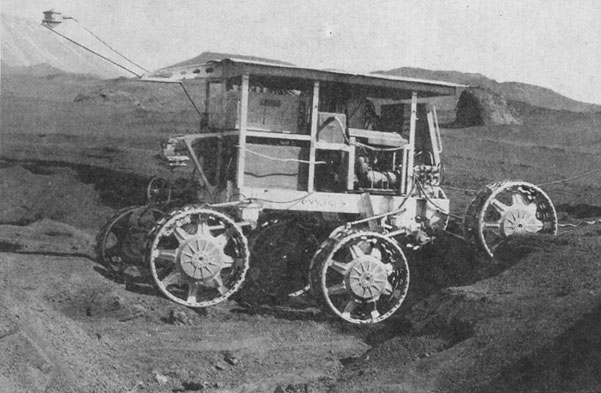
\includegraphics[width=0.7\textwidth]{from_master/vniitm}
\caption{VNIITM}
\label{fig:vniitm}
\end{figure}

\begin{figure}[H]
\centering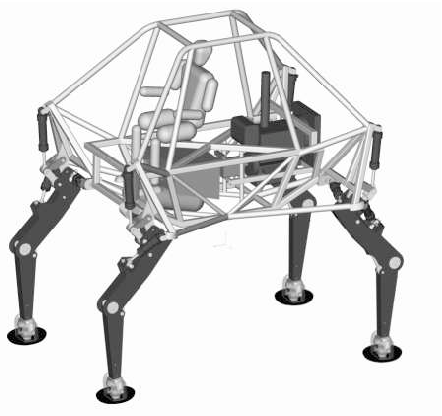
\includegraphics[width=0.6\textwidth]{from_master/alduro}
\caption{Робот Alduro}
\label{fig:alduro}
\end{figure}

\begin{figure}[H]
\centering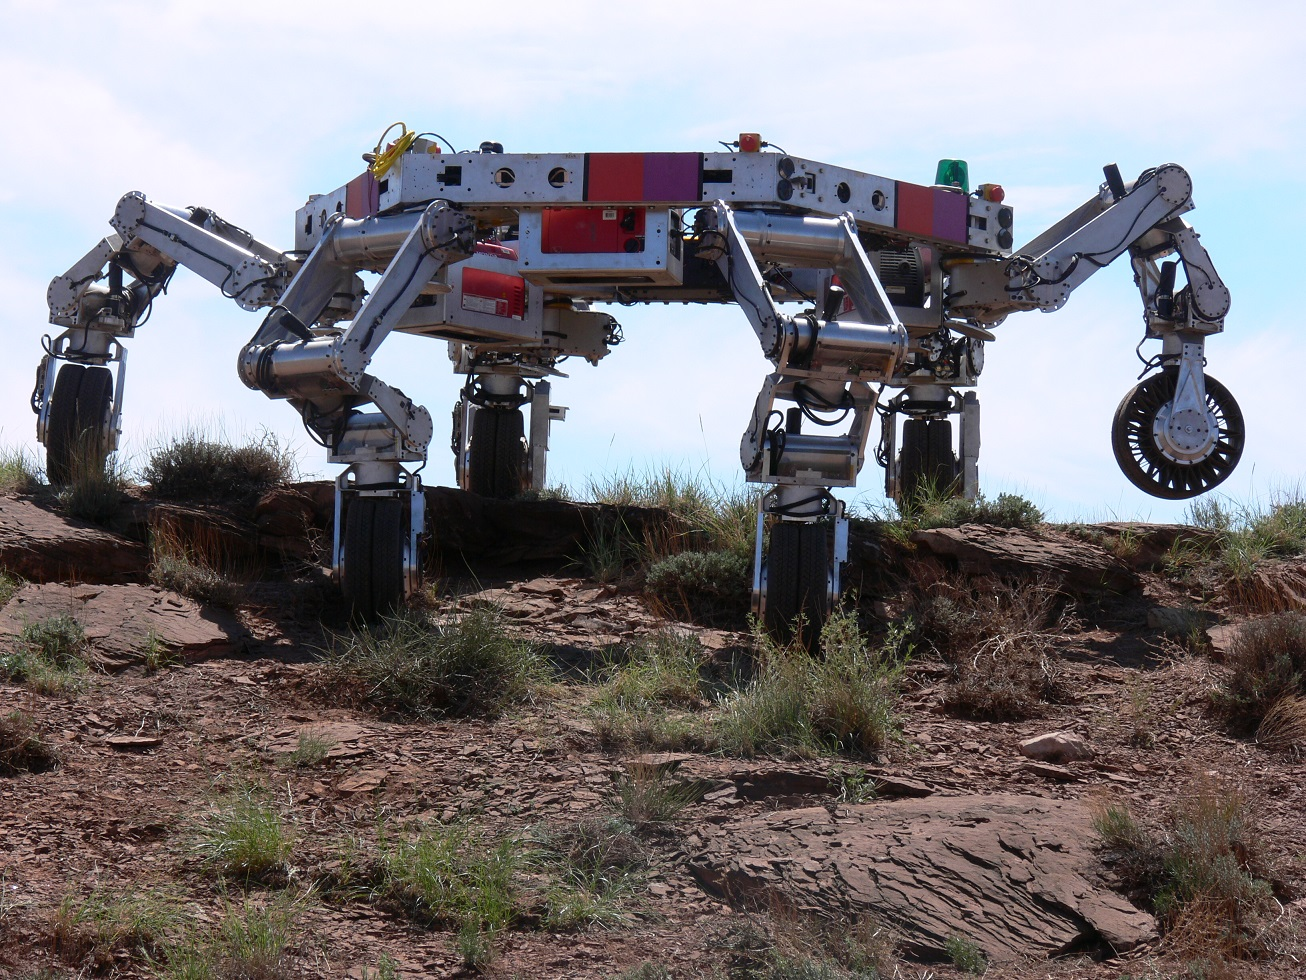
\includegraphics[width=0.6\textwidth]{from_master/athlete}
\caption{Робот Athlete}
\label{fig:athlete}
\end{figure}

Обычно тип движителей <<Прыжки и бег>> может не только прыгать или бегать, но и шагать. Примеры следующие \cite{Pavl2013,Volkova2013modeling,bidgoly2010learning,Yachun2010} \pic{fig:bigDog}.

\begin{figure}[H]
    \centering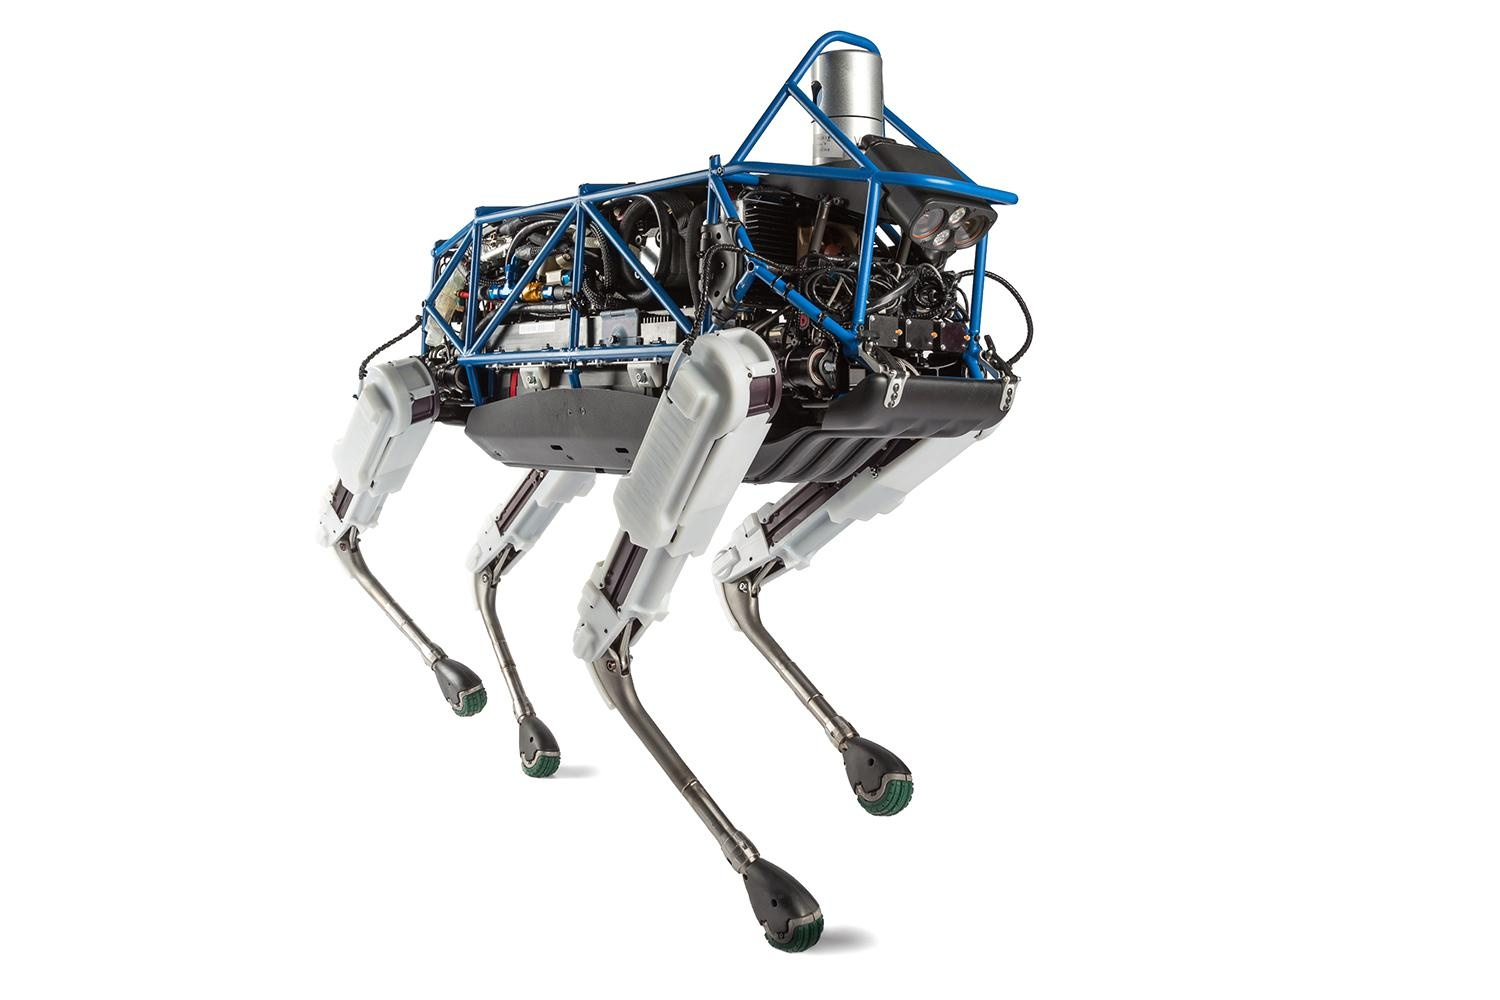
\includegraphics[width=0.8\textwidth]{from_master/bigDog}
\caption{BigDog}
\label{fig:bigDog}
\end{figure}

К машинам ползучего типа в соответствии с приведенным выше определением относится большинство так называемых шагающих экскаваторов \pic{fig:Esh6}. Несмотря на слово "шагающий" в названии, такие машины передвигаются, поднимаясь с помощью ног, и ложатся на дно при перестановке ног в новое положение.

\begin{figure}[H]
\centering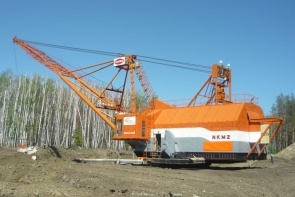
\includegraphics[width=0.7\textwidth]{from_master/Esh6}
\caption{Ползущий экскаватор российского производства}
\label{fig:Esh6}
\end{figure}

\cite{peters2010prototype,Grad2014,bidgoly2010learning} Специфика взаимодействия с опорной поверхностью и область применения лазающих машин настолько сильно отличаются, что сравнение их показателей (за исключением общетехнических) становится практически бессмысленным. Следует также отметить, что многие ползающие и лазающие роботы не имеют ног или какого-то их подобия, передвигаясь, например, за счет движений гибкого тела.

\begin{figure}[H]
\centering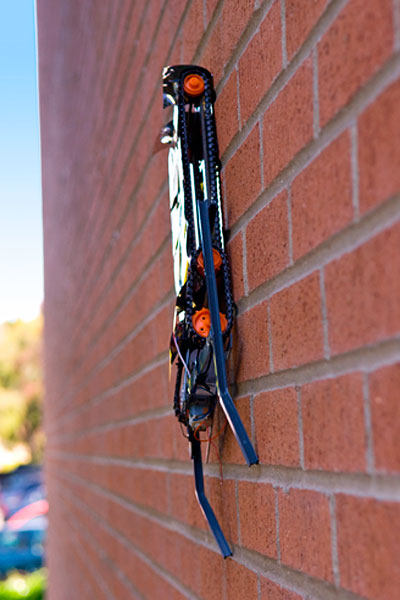
\includegraphics[width=0.45\textwidth]{from_master/brickwall}
\caption{BrickWall робот}
\label{fig:brickwall}
\end{figure}

\begin{figure}[H]
\centering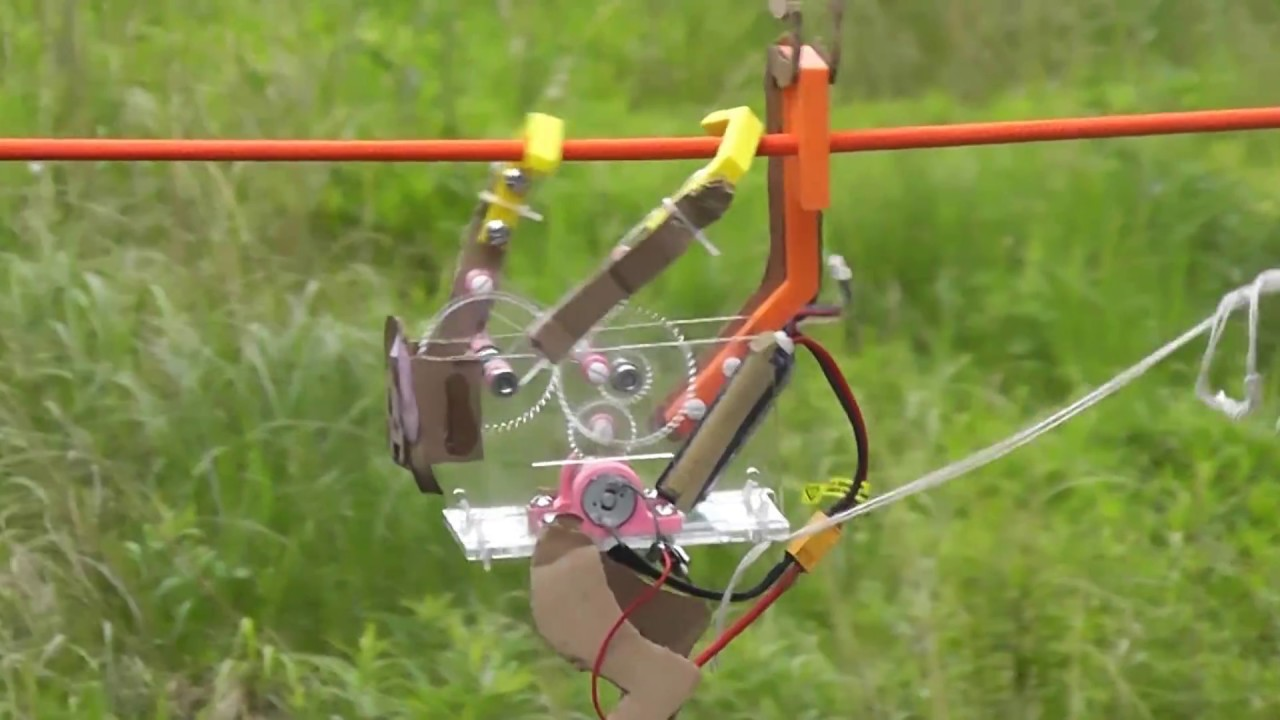
\includegraphics[width=0.7\textwidth]{from_master/ropeClimbing}
\caption{Робот, взбирающийся по канату}
\label{fig:ropeClimbing}
\end{figure}

Согласно этой классификации, предлагаемый робот относится к категории "Шагающие машины с циклическим действием движителей".

\section{Роботы, которые могут использоваться для исследования пещер}

Исследование пещер естественного происхождения является комплексной задачей, сопряженная со множественными трудностями \cite{Zhang2017a, Frumkin2019}. Деградация сенсоров \cite{Huang2019}, перебои в коммуникации между роботами из-за потери сигналов \cite{Vaquero2018, Thangavelautham2017}, сложный рельеф пещер \cite{Thangavelautham2017}, обилие грязи \cite{Baker2004}, жидких препятствий \cite{Morris2006}, требующие герметизацию корпуса, являются только малой частью встречаемых проблем в пещерах. 

В пещерах возможно встретить почти все типы поверхностей, с которыми приходится сталкиваться роботам в мире. Это и твердые поверхности: мрамор, кварц, базальт. Сыпучие грунты, такие как: мел, гипс, соль, известняк. Часто встречаются водные препятствия — как лужи, так и целы залы, погруженные в воду. Особую опасность для человека вносят сифоны. Скользкие поверхности: лед, мох, глина, а так же разрушаемые поверхности — каменная гряда и паутина \cite{1960,1963,1969,1971}. Все это вносит свои коррективы на выбор сенсоров. Так же важно понимать габариты пещер. Это влияет на необходимую автономность робототехнической системы \cite{Mascarich2018a}. 

Для преодоления сложного рельефа различные роботы, робототехнические системы и типы движителей были предложены исследователями по всему миру \cite{Morris2006a}. Разрушение пещер нежелательно, поэтому роботы, которые для перемещения ломают породу не будут рассматриваться \cite{Semini2016}. В пещерах принято использовать, как наземных роботов, так и летающие аппараты, так и их комплексы. Из летающего транспорта это коптеры \cite{Papachristos2019,Scaramuzza2014,Zingg2010} и дирижабли \cite{Huang2019}. Дирижабль намного более автономен и может нести большую нагрузку. Наземных роботов очень много типов, но основными являются: шагающие \cite{Tan2016,Lynch2019} колесные \cite{Molyneaux2016,Vaquero2018}, трековые \cite{Reddy2015} и необычные. Необычные это роботы, которые не поддаются классификации, например змеевидные \cite{Ye2007,Borenstein2007}, шарообразные \cite{Thangavelautham2017,Dubowsky2008,Dang2019} и другие.

Но самыми эффективными являются не одинокие роботы, но системы. В данных системах появляются дополнительные задачи, как архитектурного характера, телекоммуникационного и управленческого. Обычно системы состоят из нескольких одинаковых роботов \cite{Vaquero2018}, либо связка – коптер и шагающий \cite{Chen2010,Cantelli2013}.

Отдельным пластом роботов являются ползающие роботы \cite{Schmidt2013}, которые рассматриваются автором как перспективные в пещерах. К сожалению, ползащющие роботы были найдены только для космических пещер \cite{Parness2017}. 

Важным критерием для успешного робота, который может перемещаться по вертикальным поверхностям является способ адгезии с поверхностью. Существуют магнитный \cite{Lee2012,Tavakoli2012,Kotay1996,Xu2017}, электрический \cite{Li2017}[33], негативного давления \cite{Lee2012,Tavakoli2012,Papachristos2019}, пневматический или помощью присосок \cite{Nagakubo1994,Tlale2012}, и с помощью когтей (механическая адгезия) \cite{Parness2017,Bretl2006,SangbaeKim2005,Sintov2011}. Последний способ является самым применимым для пещер, так как стены очень рельефные.

Навигация в пещерах является нетривиальной задачей, поэтому рассмотрены какие сенсоры и алгоритмы, а также архитектурные решения использовались для преодоления проблем. Целесообразно рассмотреть работы в близких и смежных областях. К примеру, исследование трубопровода \cite{Savin2017}, завалов после техногенных катастроф. С точки зрения навигации основной проблемой является недостаток света, а также сильной неоднородности территории и обилия гранулированных поверхностей. На данный момент ученые мира стали стремиться решить данную проблему, благодаря проходящему соревнованию DARPA Subterranean Challenge. В данном направлении используются как лазерные дальномеры (лидары), так и визуальные SLAM алгоритмы \cite{Mascarich2018a,Dang2019a,Fairfield2006,Chhaniyara2012}. С точки зрения архитектуры, наблюдается тенденция к модульности, а также к возможным защитам от потерь робота \cite{Miller2019,Wei2009}. То есть, если робот был потерян, то остальные роботы все равно должны передавать друг другу данные. Очень важно уметь правильно передвигать робота по сыпучим грунтам, следующие работы посвящены этим проблемам. Основной критерий это решение задачи в настоящем времени \cite{Tan2016,Savin2017,Chhaniyara2012,Tsounis2019, Li2009,Bjelonic2019,DeViragh2019,Buchanan2019}.

Целью работы является разработка метода, который поможет получить информацию по поверхности пещеры. Обычно под этим подразумевается только получения типа поверхности, эти статьи и были рассмотрены \cite{Wu2016,Wu2020,Luo2017}.

Подведя итог, в данном обзоре были представлены причины проблем, возникающие при разведке пещер роботами. Были описаны типы пещер, рассмотрены их размеры. Представлены варианты возможных препятствий, а также сделаны выводы как это влияет на робототехническую систему. После этого показаны решения, предложенные исследователями по всему миру, связанные с навигацией, подбором движителя, выбором сенсоров и архитектурными решениями, дающие надежную систему. 

\subsection{Классификация шагающих машин}
Данная классификация основана на  \cite{Maloletov2015dinamica} работе. С помощью ног могут реализовываться локомоции различных типов. \textit{Ходьбой} называется такой тип движения машины, при котором в каждый момент времени хотя бы один механизм шагания находится в опоре. Если существуют такие моменты времени когда ни одна из ног машины не контактирует с опорой, то такие движения называются \textit{прыжками, скачками или бегом}. Если фаза движения машины с опорой на ноги перемежается фазой покоя, в которой машина неподвижно лежит на опорной поверхности, то такое движение называется \textit{ползанием}. Ходьба, прыжки, скачки, бег и ползание предполагают что связи ног с опорной поверхностью является неудерживающими. Однако ноги могут быть снабжены специальными устройствами — захватами, присосками и.т.п., позволяющими аппарату реализовывать удерживающие связи с опорной поверхностью. Тип движения такого аппарата называется \textit{лазанием}.

На основе данной классификации, разрабатываемый робот входит в состав группы ''Шагающие циклового действия''.

\subsection{Типы мобильных робототехнических комплексов}
Для работы на земле была разработана концепция \textit{Мобильного Робототехнического Комплекса} (МРК) -  совокупность программно-алгоритмических и аппаратных решений обеспечивающих комплексную автоматизацию выполнения группы поставленных задач.

По массе и основному назначению МРК можно разделить на четыре группы \tab{tab:mrk_types}:
\begin{itemize}
\item сверхлегкие, массой до 35 кг;
\item легкие, массой до 150 кг;
\item средние, массой до 800 кг;
\item тяжелые, массой свыше 800 кг.
\end{itemize}
\begin{small}
\begin{center}
\begin{longtable}[H]{|p{2cm}|p{3cm}|p{3cm}|p{3.2cm}|p{3cm}|}
%Костылина для таблиц, чтобы по ГОСТу было название
\caption{Классификация МРК }\\
\label{tab:mrk_types}
% \multicolumn{5}{l}%
% {\normalsize{Таблица \thetable ~--- Классификация МРК} \label{tab:mrk_types}}\\
% \hline
\normalsize{Группа} & \normalsize{Назначение} & \normalsize{Мобильность} & \normalsize{Особенности конструкции} & \normalsize{Оснащение}\\
\hline
\endfirsthead
\multicolumn{5}{l}%
{\textit{\normalsize{Продолжение таблицы \thetable}}}\\
\hline
\normalsize{Группа} & \normalsize{Назначение} & \normalsize{Мобильность} & \normalsize{Особенности конструкции} & \normalsize{Оснащение}\\
\hline
\endhead
\hline
\endlastfoot
\normalsize{Сверх\-легкие} 
&
Визуальная и акустическая разведка в помещениях и в объектах транспорта. Осмотр труднодоступных мест (днища автомобилей и т.п.) и разрушение обнаруженных СВУ.
&
Перевозка любым видом транспорта в контейнере-чемодане. Выгрузка оператором. Переноска оператором или доставка с помощью более тяжелых МРК к исследуемому объекту. 
&
Шасси гусеничное, колесное или специальное комбинированное. Управление по радио, волоконно-оптической линии связи (ВОЛС) или кабелю. Питание от аккумуляторов. 
&
1-4 малогабаритных черно-белых или цветных камеры 
1-2 гидроразрушителя. \\ 
\hline 
\normalsize{Легкие}
&
Разведка внутри помещений и на открытой местности. Проведение взрывотехнических работ.
&
Перевозка легковым автомобилем с кузовом <<универсал>>. Выгрузка вручную (2-4 чел.) или своим ходом по аппарелям. Возможна переноска на относительно небольшие расстояния.
&
Шасси гусеничное, колесное или специальное комбинированное. Управление по радио, ВОЛС или кабелю. Питание от встроенных аккумуляторов или от сети по кабелю до 100 м.
&
1-4 телекамеры. Стрела кранового или телескопического типа, либо манипулятор с 2-5 степенями подвижности. самозарядное ружье. комплекты взрывотехнического и разведывательного оборудования. \\ 
\hline 
\normalsize{Средние} 
&
Разведка, наблюдение, охрана, проведение взрывотехнических работ. Носитель легкого стрелкового и ракетного вооружения.
&
Перевозка микроавтобусом или легким грузовиком. выгрузка своим ходом по аппарелям.
&
Шасси гусеничное, колесное или специальное комбинированное. Управление по радио, ВОЛС или кабелю. Питание от встроенных аккумуляторов 
&
2-4 телекамеры. Манипулятор с 2-6 степенями подвижности и сменным инструментом. Самозарядное ружье, пулемет, гранатомет, ракетная пусковая установка. \\ 
\hline 
\normalsize{Тяжелые}
&
Разведка, наблюдение, патрулирование, проведения взрывотехнических работ. Носитель легкого пушечного и тяжелого стрелкового вооружения
&
Перевозка на большие расстояния специальным автотранспортом или в стандартных транспортных контейнерах. Выгрузка своим ходом или с помощью крана.
&
Шасси гусеничное, колесное или специальное комбинированное. Возможно использование серийно выпускаемых транспортных средств. Управление по радио, ВОЛС или кабелю;  
&
3-4 камеры. Манипулятор с 4-6 степенями подвижности и сменным инструментом. Пулемет, малокалиберная автоматическая пушка. Комплекты взрывотехнического и разведывательного оборудования. \\  
\hline 
\end{longtable}
\end{center}
\end{small}

Разрабатываемый робот принадлежит к сверхлегким роботам.

\subsection{Исследования с похожими роботами}
Гексаподы - это особая форма насекомых. Эта форма представляет собой минимальную по количеству ног модель, которая демонстрирует качественное поведение сороконожки. Более того, были интересные попытки создать гибриды между колесными роботами и многоножками, чтобы получить "лучшее из обоих миров".

Boston Dynamics RHex \cite{altendorfer2001rhex} - это шестиногий робот \pic{fig:rhex}, тело которого похоже на модель робота, которую будет использоваться. Независимо управляемые ноги создают специальные походки, которые перемещают его по неровной местности, такой как лестница, каменная гряда и т.д. Одна из походок обеспечивает возможность прыжка. Форма ног обеспечивает плавность движений. Однако у робота есть и ряд недостатков. Прежде всего, это высокое энергопотребление, так как он содержит шесть двигателей. Кроме того, у этого робота есть некоторые трудности с управляемостью. 

\begin{figure}[H]
    \centering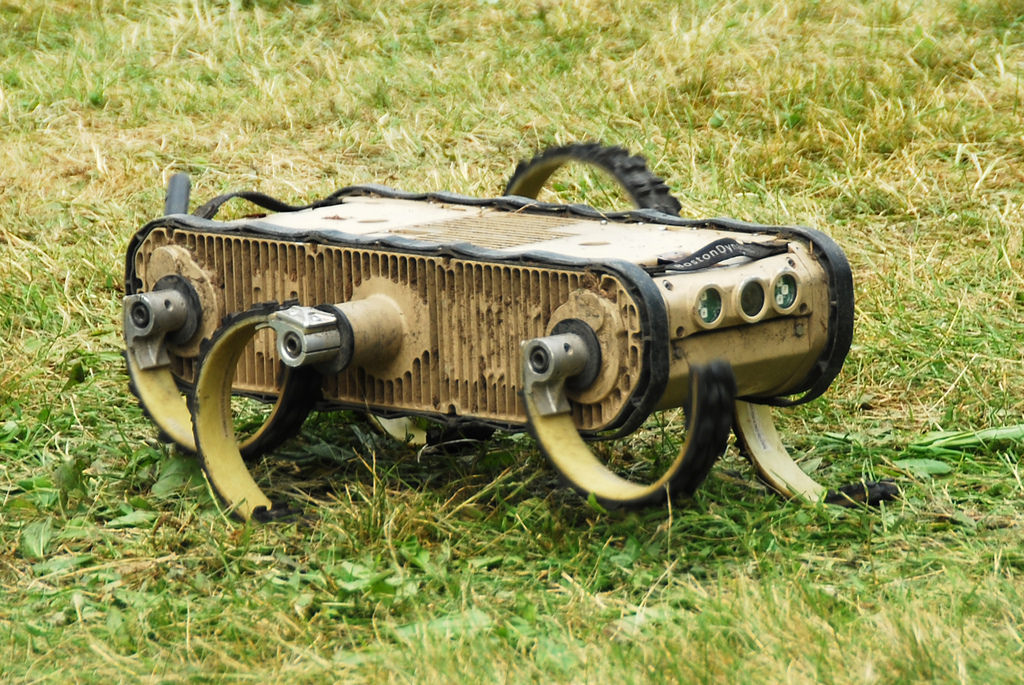
\includegraphics[width=0.4\textwidth]{from_master/rhex}\\
    \caption{Boston Dynamics робот RHex}
    \label{fig:rhex}
    \end{figure}

Gakken Mechamo Centipede \cite{miller2008extreme} - робот \pic{fig:gakken}, который имеет схожую кинематическую схему с моделью робота, разработанной в данной работе. Большое количество ног может обеспечить ему хорошую проходимость на пересеченной местности, и потеря ноги не будет критичной для робота. Однако это снижает долговечность компонентов робота. Кроме того, небольшая высота ноги снижает возможности передвижения по пересеченной местности.
\begin{figure}[H]
    \centering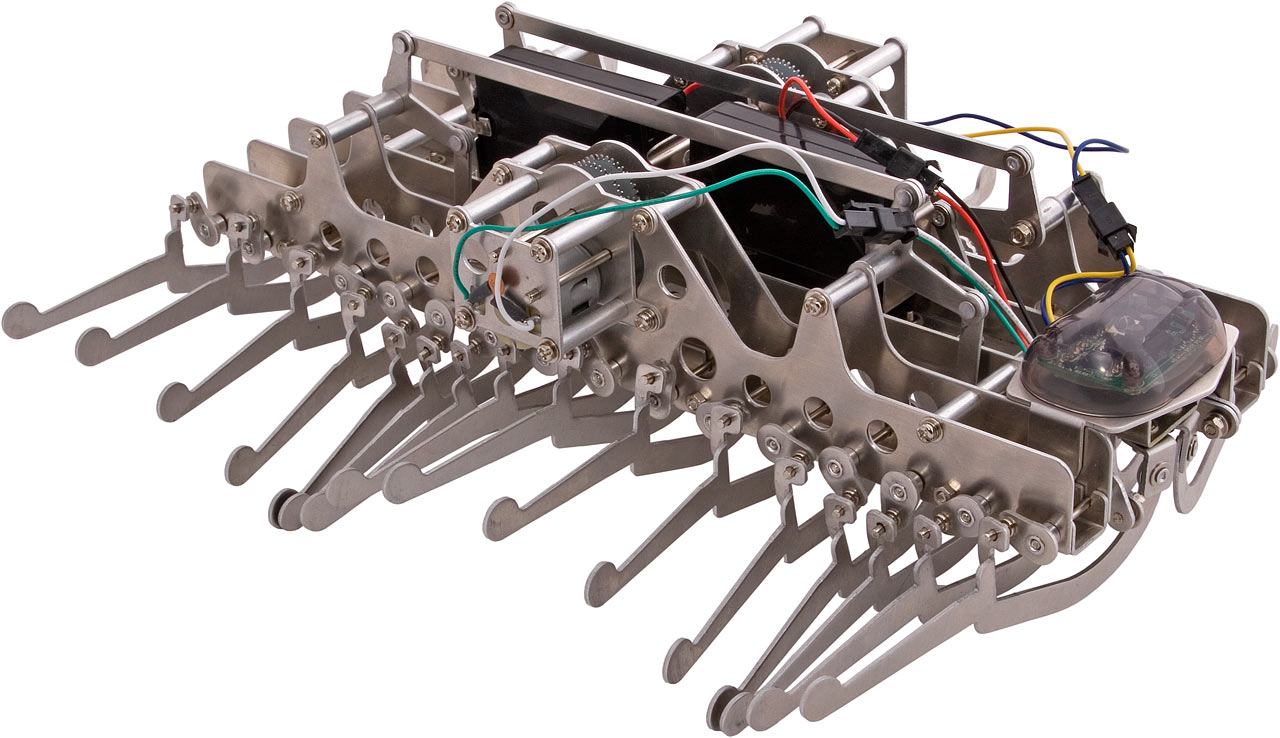
\includegraphics[width=0.5\textwidth]{from_master/gakken}\\
    \caption{Gakken Mechamo Centipede робот}
    \label{fig:gakken}
    \end{figure}

Quattroped \cite{chen2014quattroped,chen2017turboquad} и TurboQuad - это роботы, трансформирующие колеса в ноги \pic{quatro}. Когда он использует ноги, его кинематическая схема похожа на робота RHex, в случае режима работы колес он похож на транспортное средство. Он обеспечивает высокую скорость на ровной местности, но конструкция робота становится очень сложной, что снижает его устойчивость. Всего четыре ноги, в некоторых случаях, делают робота неустойчивым.

\begin{figure}[H]
    \begin{subfigure}{0.49\textwidth}
    \centering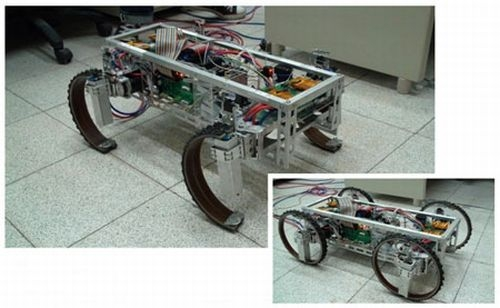
\includegraphics[width=0.9\textwidth]{from_master/quattroped}\\
    \caption{Quattroped robot}
    \label{fig:quattroped}
    \end{subfigure}
    \begin{subfigure}{0.49\textwidth}
    \centering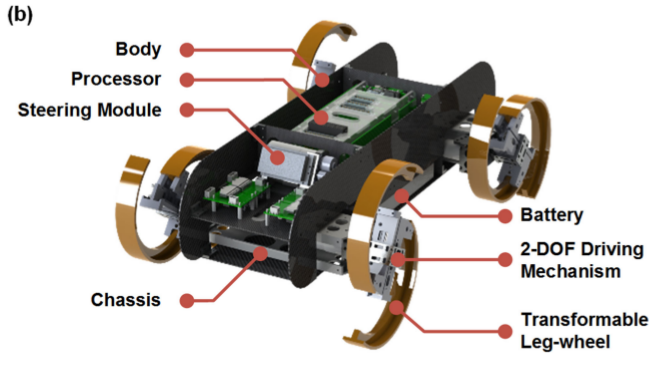
\includegraphics[width=0.9\textwidth]{from_master/turboquad}\\
    \caption{TurboQuad robot}
    \label{fig:turboquad}
    \end{subfigure}
    \caption{Quattroped семья роботов}
    \label{quatro}
    \end{figure}

Whegs \cite{schroer2004comparing} \pic{fig:whegs} использует стратегию локомоции, которая сочетает простоту колеса с преимуществами преодоления препятствий ногой. Несмотря на разницу в высоте ног по сравнению с роботом RHex, в некоторых случаях. Колеса могут обеспечить те же возможности движения. Это стало возможным благодаря использованию сегментированного тела. С другой стороны, эта особенность делает робота более сложным в производстве и управлении.

\begin{figure}[H]
\centering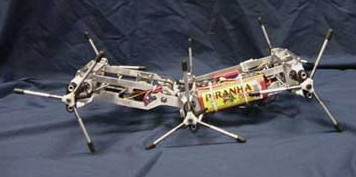
\includegraphics[width=0.7\textwidth]{from_master/whegs2.jpg}\\
\caption{Whegs II robot}
\label{fig:whegs}
\end{figure}

Сравнительный анализ между представленными выше роботами приведен в таблице \ref{tabular:robot_comparison}.
\begin{table}[H]
    \centering
\caption{Сравнительный анализ гесаподов}
\label{tabular:robot_comparison}
% \begin{center}
\begin{small}
\begin{tabular}{l|c|c|c|c}
\toprule
\toprule
\rowcolor{Gray}
 Parameters & RHex & \makecell{Gakken \\ Mechamo\\ Centipede} &  \makecell{Quat-\\troped} & \makecell{Whegs \\ II}\\
 \hline
Длина, мм & 540 & 320 & 600 & 470 \\ 
  \rowcolor{LightGray}
 Ширина, мм & 200 & 140 & 190 & 360 \\
 Высота, мм & 127 & 100 & 140 & 50 \\
  \rowcolor{LightGray}
 Масса, кг & 8.2 & 1.1 & 8.6 & 3.86 \\ 
 Количество ног & 6 & 32 & 4 & 18 \\
  \rowcolor{LightGray}
 Высота ноги, мм & 175 & 50 & 175 & 100  \\
 Масса ноги, кг & 0.1 & 0.02 & 0.38 & 0.05 \\
  \rowcolor{LightGray}
 скорость, м/с & 1.6 & 0.1 & 2 & 1.5 \\
\bottomrule
\bottomrule
\end{tabular}
\end{small}
% \end{center}
\end{table}

Все эти роботы, кроме Gakken Centipede, были созданы для разведки, и значения их параметров можно легко объяснить. Такая ширина должна быть меньше размера двери. Еще лучше, если ширина робота будет меньше 2/3 размера двери, и все прототипы удовлетворяют этому условию. При навигации внутри помещений длина также имеет некоторые ограничения, иначе он не сможет передвигаться в коридорах и тесных помещениях. Масса зависит от других параметров. Высокая скорость не нужна в помещениях и опасных зонах. 

Похожие роботы, такие как Boston Dynamics RHex \cite{altendorfer2001rhex}, Gakken Mechamo Centipede \cite{miller2008extreme}, Quattroped and TurboQuad \cite{chen2014quattroped,chen2017turboquad}, а так же Whegs \cite{schroer2004comparing} были рассмотрены. На основе данных было решено, что робот должен быть в длину меньше метра, в ширину --- меньше 70 см (стандартная ширина дверного проема). Иметь меньше 32 лапок и высота лапки должна быть больше 10 см.



\section{Описание пещеры}
Пещера -- полость в верхней части земной коры, сообщающаяся с поверхностью одним или несколькими входными отверстиями. Пещеры естественного происхождения бывают:
\begin{itemize}
    \item карстовые; 
    \item тектонические;
    \item эрозионные;
    \item ледниковые;
    \item вулканические.
\end{itemize}

Структуры поверхностей:
\begin{itemize}
    \item твердые породы, прочные -- мрамор, кварц, базальт (магма) \pic{fig:solid_surfaces};
    \item твердые породы, мягкие -- мел, гипс, соль, известняк \pic{fig:solid_surfaces};
    \item сыпучие грунты -- песок, глина, снег \pic{fig:running_soils};
    \item водные преграды -- как и лужи (малый слой воды), залы, погруженные под воду. Встречаются сифоны \pic{fig:water_obstacles};
    \item скользкие поверхности -- отложения мха и плесени, лед \pic{fig:slippery_surfaces};
    \item разрушаемые поверхности -- каменная гряда, паутина.
\end{itemize}


\begin{figure}[H]
\begin{subfigure}{0.49\textwidth}
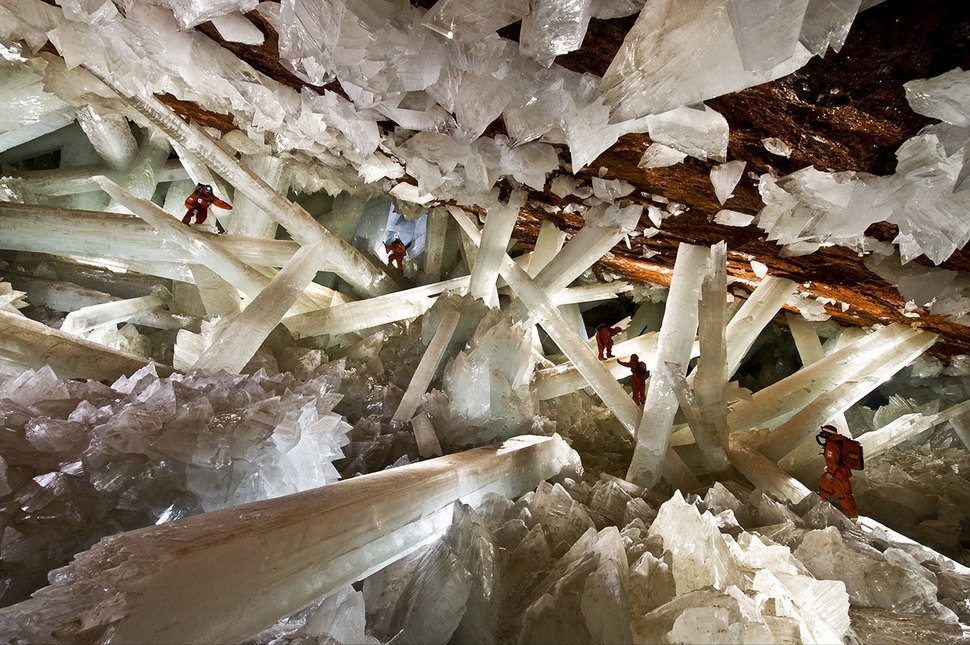
\includegraphics[width=0.99\textwidth]{surface_types/crystal.png}\\
\caption{Кристаллы}
\label{fig:crystal}
\end{subfigure}
\begin{subfigure}{0.49\textwidth}
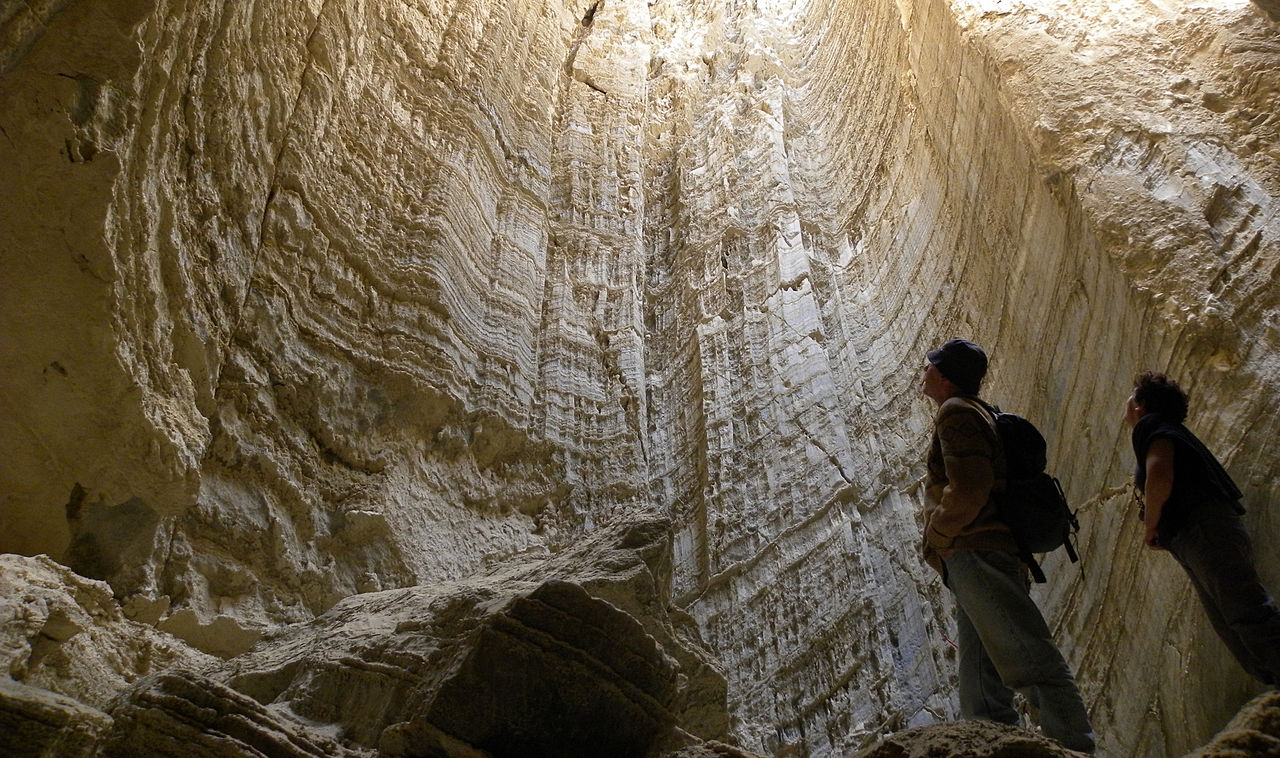
\includegraphics[width=0.99\textwidth]{surface_types/salt.jpg}\\
\caption{Солевые отложения}
\label{fig:salt}
\end{subfigure}

\begin{subfigure}{0.49\textwidth}
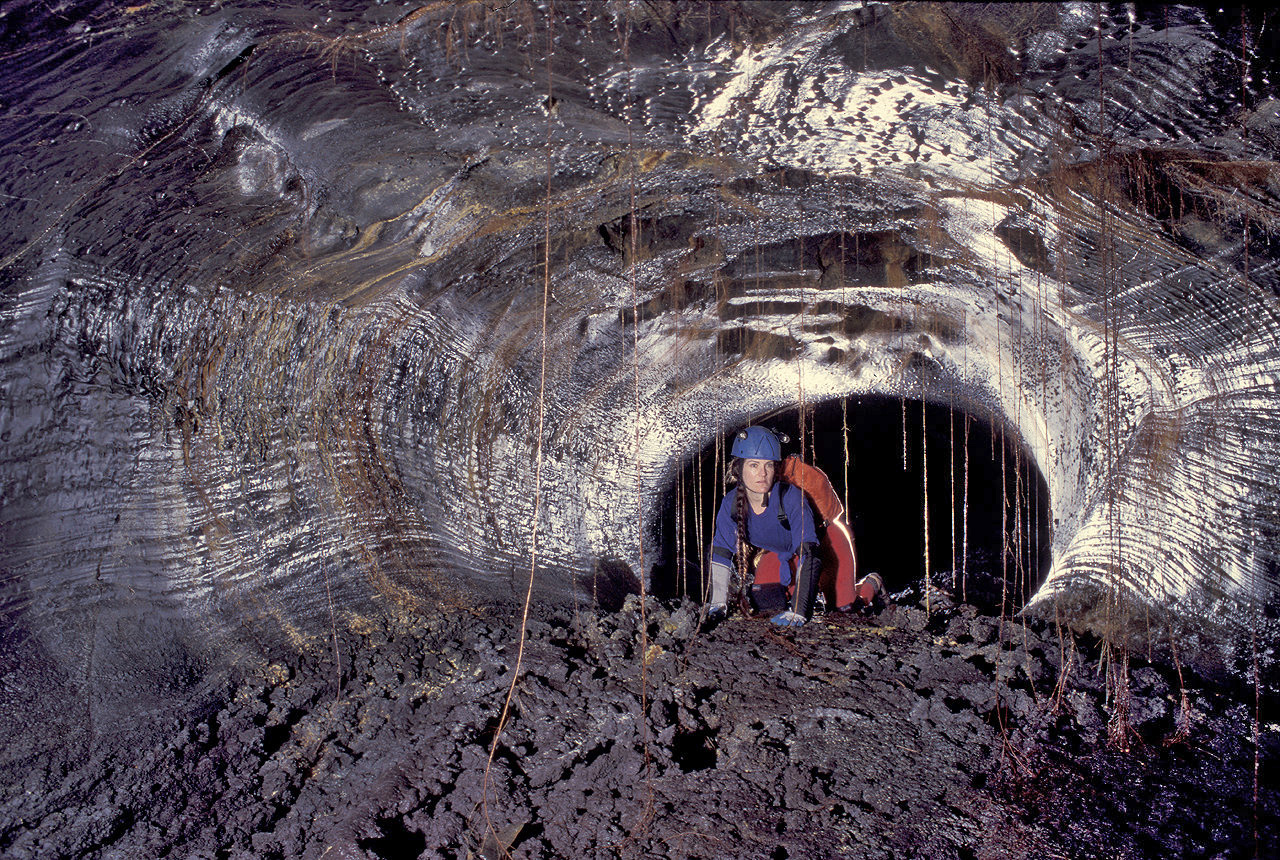
\includegraphics[width=0.99\textwidth]{surface_types/lava.jpg}\\
\caption{Магма}
\label{fig:lava}
\end{subfigure}
\begin{subfigure}{0.49\textwidth}
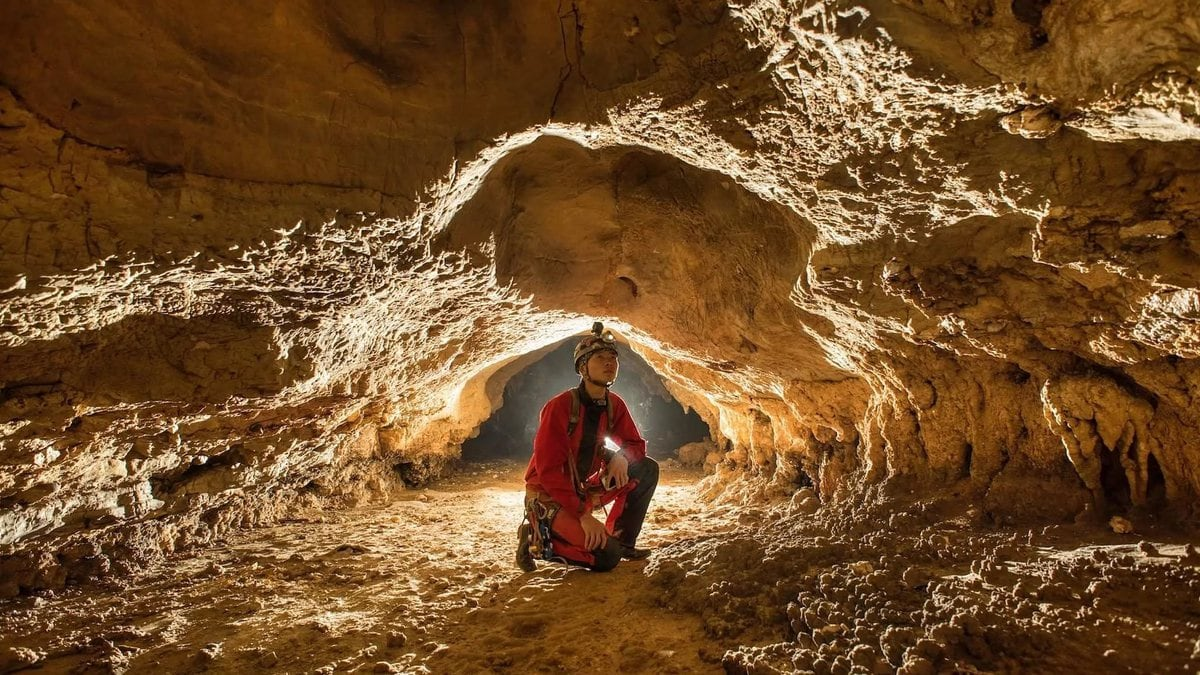
\includegraphics[width=0.99\textwidth]{surface_types/limestone.png}\\
\caption{Известняк}
\label{fig:limestone}
\end{subfigure}
\caption{Твердые поверхности}
\label{fig:solid_surfaces}
\end{figure}

\begin{figure}[H]
\begin{subfigure}{0.49\textwidth}
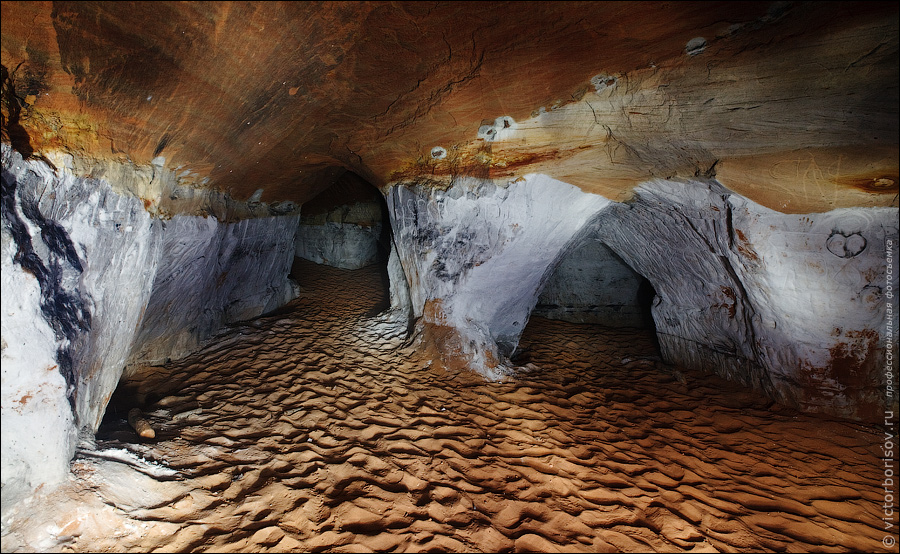
\includegraphics[width=0.99\textwidth]{surface_types/sand.jpg}\\
\caption{Песок}
\label{fig:sand}
\end{subfigure}
\begin{subfigure}{0.49\textwidth}
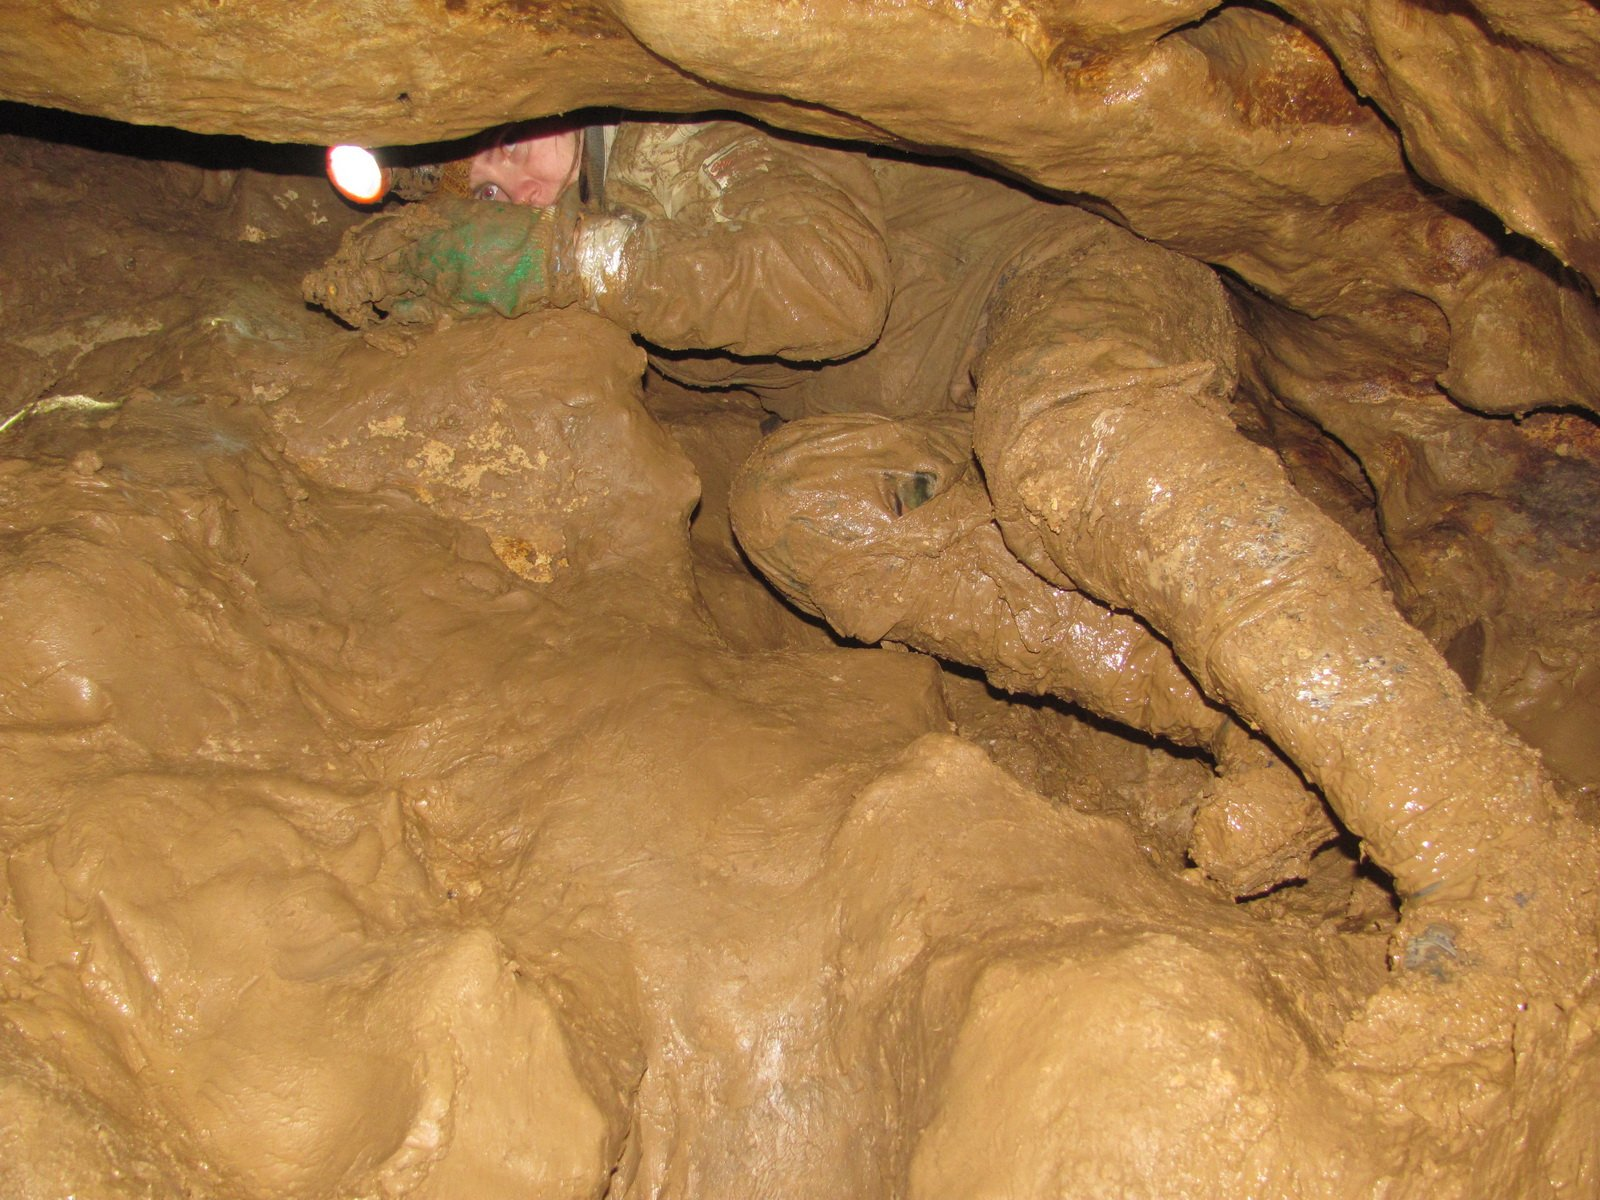
\includegraphics[width=0.99\textwidth]{surface_types/clay.jpg}\\
\caption{Глина}
\label{fig:clay}
\end{subfigure}
\caption{Сыпучие грунты}
\label{fig:running_soils}
\end{figure}

\begin{figure}[H]
\begin{subfigure}{0.49\textwidth}
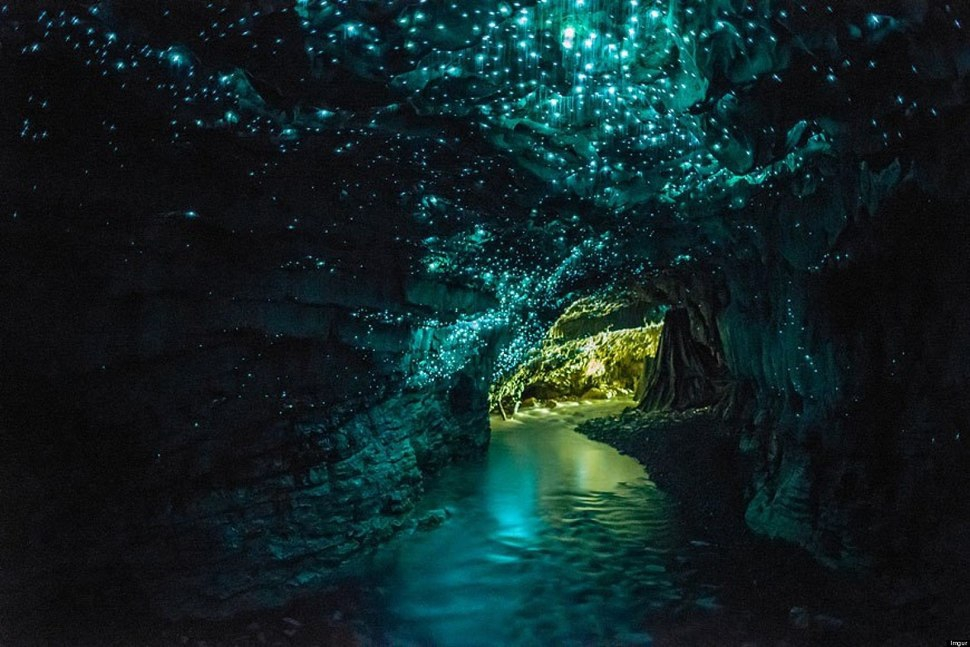
\includegraphics[width=0.99\textwidth]{surface_types/splash.png}\\
\caption{Лужа}
\label{fig:splash}
\end{subfigure}
\begin{subfigure}{0.49\textwidth}
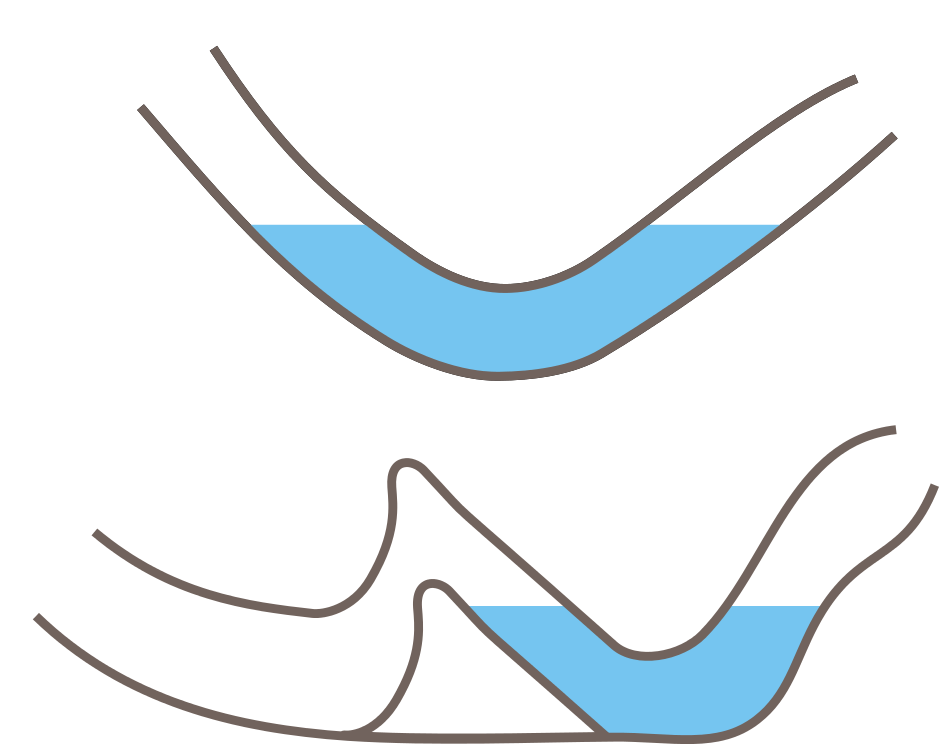
\includegraphics[width=0.99\textwidth]{surface_types/siphon.png}\\
\caption{Сифон}
\label{fig:siphon}
\end{subfigure}
\caption{Водяные препятствия}
\label{fig:water_obstacles}
\end{figure}

\begin{figure}[H]
\begin{subfigure}{0.49\textwidth}
\centering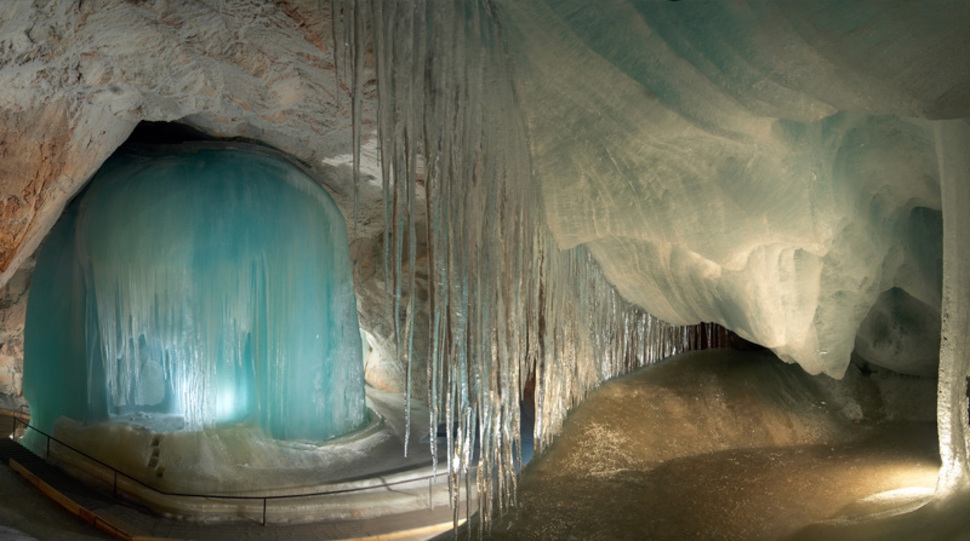
\includegraphics[width=0.99\textwidth]{surface_types/ice.png}\\
\caption{Ледяная пещера}
\label{fig:icee}
\end{subfigure}
\begin{subfigure}{0.49\textwidth}
\centering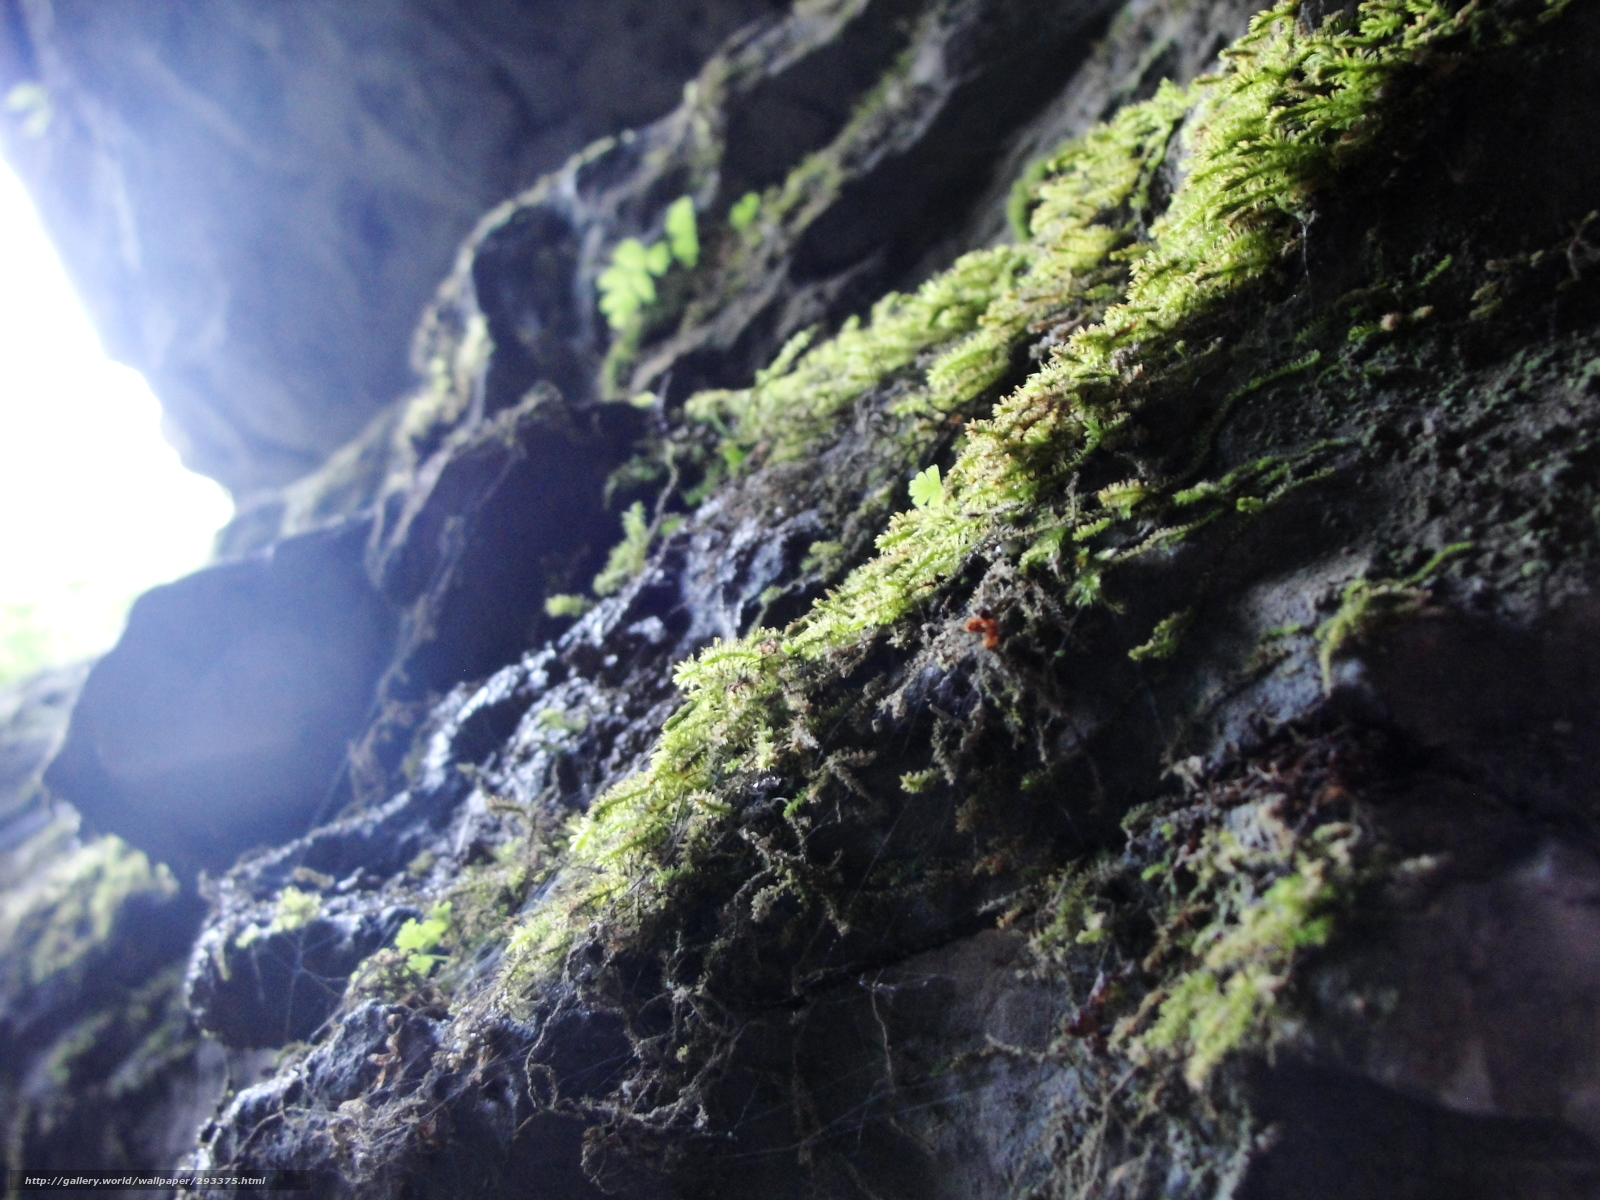
\includegraphics[width=0.99\textwidth]{surface_types/moss.jpg}\\
\caption{Мох}
\label{fig:moss}
\end{subfigure}
\caption{Скользящие поверхности}
\label{fig:slippery_surfaces}
\end{figure}

Ниже представлены размеры нескольких пещер, для того, чтобы понимать необходимый запас хода, размеры робототехнического комплекса.

\begin{figure}[H]
\begin{subfigure}{0.8\textwidth}
\centering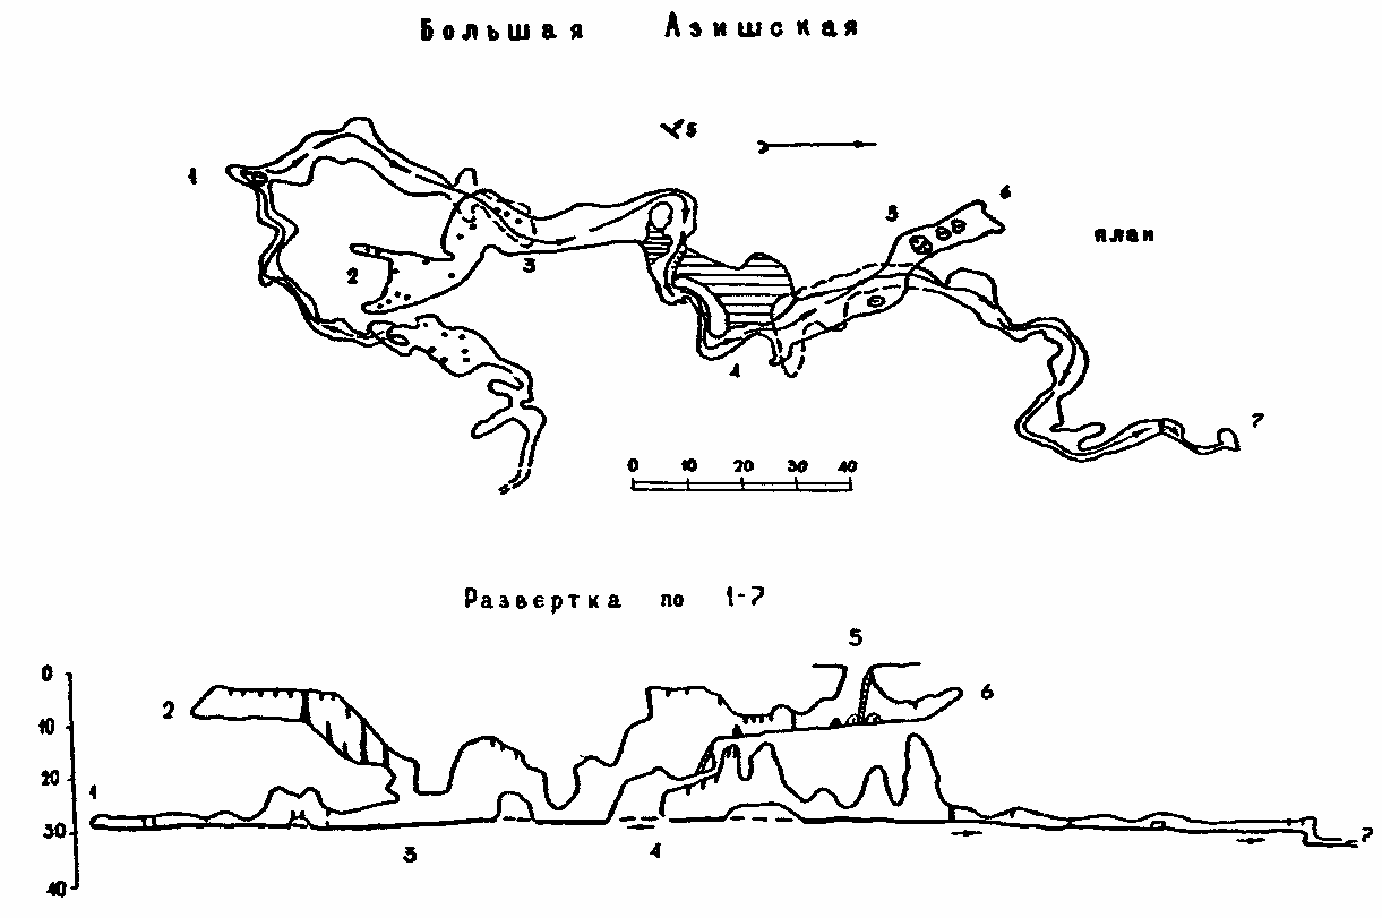
\includegraphics[width=0.8\textwidth]{cave_maps/map1.png}\\
\caption{Большая Азишская пещера}
\label{fig:ice}
\end{subfigure}
\begin{subfigure}{0.8\textwidth}
\centering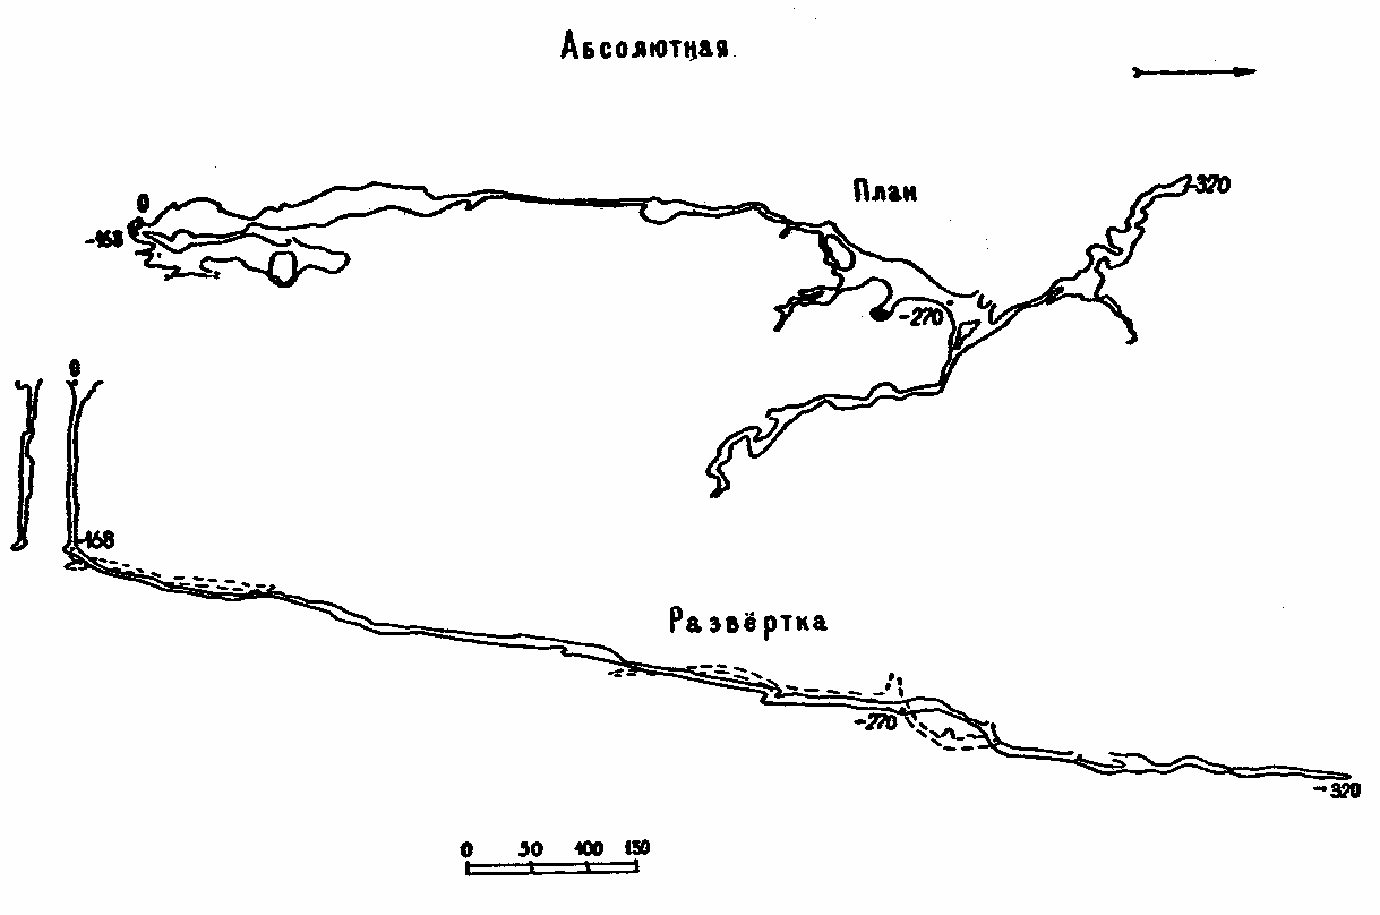
\includegraphics[width=0.8\textwidth]{cave_maps/map2.png}\\
\caption{Абсолютная пещера}
\end{subfigure}
\begin{subfigure}{0.8\textwidth}
\centering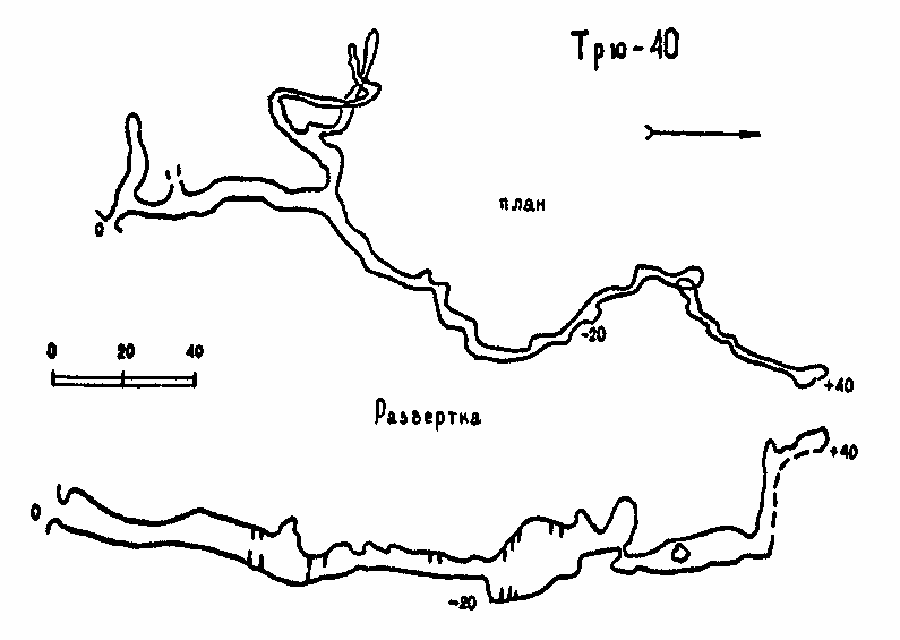
\includegraphics[width=0.8\textwidth]{cave_maps/map3.png}\\
\caption{Трю - 40}
\end{subfigure}
\caption{Размеры пещер}
\end{figure}

Определять габариты робота по картам дает нам понимание только верхней границы размеров робота, так как задача стоит в исследовании мест, куда человек не может попасть со своими габаритами.



\section{Классификация сенсорных устройств}
Информация, поступающая с различных сенсорных устройств, используется в системе управления робота для обнаружения и распознавания объектов внешней среды, построения модели, а также для управления движением робота и его манипуляторов при выполнении различных технологических операций. В соответствии с этим указанные выше две группы сенсорных устройств можно ' описать иначе следующим образом: для выявления свойств внешней среды, отдельных объектов и обеспечения перемещения исполнительных органов.

К первой из указанных групп относятся сенсорные устройства, предназначенные для выявления различных физико-химических свойств объектов среды, включая в частности устройства для выявления параметров рельефа в рабочей зоне подвижных роботов, специальных признаков для обнаружения и распознавания определенных объектов, положения и их ориентации в рабочей зоне относительно робота и т. п.

Ко второй группе относятся датчики обратной связи (положения, скорости, ускорения), усилий, возникающих при взаимодействии робота с внешней средой, прикосновения, проскальзывания и т. д.

Такое разделение сенсорных устройств достаточно условно, поскольку, например, сенсорные устройства первой группы могут быть использованы и для определения положения захвата манипулятора робота в рабочей зоне, т. е. играть роль датчиков обратной связи при управлении движением.

Сенсорные устройства робота могут воспринимать информацию на различных расстояниях от ее источника. По этому признаку сенсорные устройства делятся на сверхближние, ближние, дальние и сверхдальние (работающие вне рабочей зоны).

Сенсорные устройства сверхближнего действия используют для очувствления захватов и других частей манипуляторов, а также корпуса робота. Они позволяют фиксировать их контакт с объектами внешней среды (тактильные датчики), измерять усилия, возникающие в месте взаимодействия (силометрические датчики), фиксировать проскальзывание объектов.

Сенсорные устройства ближнего действия обеспечивают получение необходимой информации в непосредственной близости от робота, но бесконтактным способом. К таким устройствам относятся локационные сенсоры захвата, неконтактные бамперы, различные дальномеры ближнего действия, измерители плотности грунта и т. п. Бесконтактные измерительные устройства технически сложнее контактных, но позволяют роботу выполнять задание с большей скоростью, заранее получать информацию о ближайших объектах и соответствующим образом корректировать свои действия.
Сенсорные устройства дальнего действия дают информацию о внешней среде и объеме всей рабочей зоны робота.

Сенсорные устройства сверхдальнего действия применяют главным образом в подвижных роботах. К таким устройствам относятся различные навигационные устройства, координаторы, локаторы и другие оптические, радиотехнические и телевизионные системы.

В бесконтактных сенсорных системах роботов для получения требуемой информации могут быть использованы излучаемые таким устройством специальные сигналы (оптические, радиотехнические, радиационные и т. п.) или естественные излучения среды и отдельных ее объектов. В зависимости от этого различают активные и пассивные сенсорные системы. Первые обязательно включают передающие устройства, излучающие первичный сигнал, и приемные устройства, регистрирующие прямой сигнал, прошедший через среду, или вторичный сигнал, отраженный от объектов среды. Пассивные системы имеют только приемное устройство, а роль излучателя играют сами объекты внешней среды. Поэтому такие устройства технически обычно проще и дешевле, но зато и менее универсальны. Существуют также полуактивные сенсорные устройства, в которых в результате излучения внешней среды инициируется вторичное излучение ее объектов, принимаемое приемными устройствами, как в пассивных системах.
 
Таким образом на основе классификации, решено выбрать силомоментные датчики для решения поставленной задачи.

\section{Обзор триангуляций}
Для решения задачи построение карты с помощью тактильного очувствления решено генерировать поверхность на основе полученных точек. Эту задача переформулируется следующим образом. Необходимо получить оболочку из набора точек, полученных с лап робота. Оболочка, так как точно известно, что эта поверхность проходима (облако точек получено с пройденной поверхности). 

Но предварительно нужно выставить несколько тезисов для выбора правильного алгоритма \cite{ebertInterpolationExtrapolationComparison2014,kumarSurfaceTriangulationSurvey,aurenhammerVoronoiDiagramsSurvey1991}.
\begin{itemize}
    \item Граница вокруг объекта должна быть произвольной формы, а не выпуклой. Более подробно этот тезис объясняется в главе \nameref{ch:ch4}.
    \item Существует только одно скопление объектов, а все, что выходит за его пределы, считается экстраполяцией. 
    \item Плотность объектов не играет роли.
\end{itemize}

Область интерполяции \cite{brooksCharacterizingDomainRegression1988,patelLinearProgramDetect1995,baranyiEffectsParameterizationPerformance1996,haffnerEscapingConvexHull2001,kingDangersExtremeCounterfactuals2006} --- это когда одна группа объектов или набор данных является базой для определения диапазона значений для интерполяции и заключена в некую границу выпуклой формы. Область за пределами этой границы или корпуса обозначается как область экстраполяции. Обычно его называют выпуклой оболочкой. В редких случаях авторы применяют определение экстраполяции к области между несколькими группами объектов. Пример использования метода кластеризации для определения новых точек данных в области экстраполяции для обнаружения повреждений при изменяющихся условиях окружающей среды и эксплуатации для мониторинга состояния конструкций.

Еще есть случай, когда оболочка вокруг одной группы объектов не обязана иметь выпуклую форму \cite{rejerHypertubePossibleInterpolation2006,j.a.leonardUsingRadialBasis1992,verleysenLearningHighdimensionalData2001}.

В текущем случае необходимо использовать вогнутую оболочку, но чаще всего алгоритм вогнутых оболочек использует выпуклую оболочку и модифицирует ее.

Первыми алгоритмами для вычисления выпуклых оболочек были Алгоритм Грэхема \cite{grahamEfficientAlgorithDetermining1972} и Алгоритм Джарвиса \cite{jarvisIdentificationConvexHull1973}, которые были усовершенствованы в \cite{chanOptimalOutputsensitiveConvex1996}. Все эти алгоритмы были ограничены проблемами низкой размерности. 

Для получения выпуклого оболочки большей размерности был предложен алгоритм Алгоритм быстрой оболочки \cite{clarksonApplicationsRandomSampling1988}. Современные рассматривают более комплексные области применения. Динамические выпуклые оболочки, аппроксимация оболочки для больших наборов данных, алгоритмы выпуклых оболочек для больших размерностей \cite{brodalDynamicPlanarConvex2002,khosravaniSimpleAlgorithmConvex2013,zhongFindingConvexHull2014}. Так как для задач беспилотных автомобилей и других задач подобного толка требуется решения данной задачи в режиме реально времени, авторы разрабатывают усовершенствования производительности алгоритмов путем распараллеливания и использования графического процессора (GPU) для определения внутренних точек \cite{zhongFindingConvexHull2014,cintraSpeculativeParallelizationRandomized2004,cintraSpeculativeParallelizationRandomized2004,tangSMI2012Full2012,tzengFindingConvexHulls2012}.

Как говорилось выше, в нашей задаче важнее рассмотрить алгоритмы для построения вогнутых оболочек. Существует несколько различных подходов к вычислению границ произвольной формы. Основные концепции алгоритмов построения вогнутых корпусов основаны на методах ближайших соседей, ядерных функциях или триангуляции Делоне. Хотя это не совсем алгоритмы для построения вогнутой оболочки, существует также область статистических подходов в определении признаков новизны, которая решает ту же проблему. 

Известным алгоритмом для построения вогнутой оболочки является $\alpha$-shapes \cite{edelsbrunnerShapeSetPoints1983,edelsbrunnerThreedimensionalAlphaShapes1992}. Это обобщение вогнутой оболочки, где $\alpha$ - параметр, и по мере приближения $\alpha$ к 0, $\alpha$-оболочка приближается к обычной выпуклой оболочке. $\alpha$-оболочки строятся из диаграмм Вороного. Есть альтернатива --- $\chi$-фигуры \cite{duckhamEfficientGenerationSimple2008}. Алгоритм $\chi$-форм является простым, гибким и эффективным для построения возможно невыпуклого простого многоугольника, который характеризует форму набора входных точек на плоскости, называемую характерной формой. Вместо диаграмм Вороного алгоритм основан на триангуляции точек по методу Делоне. Есть еще модификации на основанные на алгоритме Грэхема \cite{xuConcaveHullAlgorithm2010} с унаследованными ограничениями. 

Другой подход представлен ученым Парком \cite{parkNewConcaveHull2012}, который начинается с выпуклой оболочки и применяет алгоритм "копания". Благодаря работе \cite{j.a.leonardUsingRadialBasis1992} и появлениюю метода машинного обучения  SVM, возник новый класс методов обнаружения. Однако одноклассовые SVM не дают точной оболочки, и для различения между внутренним и внешним необходимо задать порог. С дополнительной информацие возможна двухклассовая SVM. 

Для вычисления независимых оболочек для нескольких групп объектов предлагается алгоритм с использованием алгоритма кластеризации общих ближайших соседей (SNN) , который вычисляет оболочку для каждой группы, применяя подход k-nearest neighbors (kNN) \cite{moreiraConcaveHullKnearest2007,ertozNewSharedNearest2002,chauBorderSamplesDetection2011,xiaBORDEREfficientComputation2006}.

\section{Обзор существующей системы}
\begin{figure}[H]
    \centering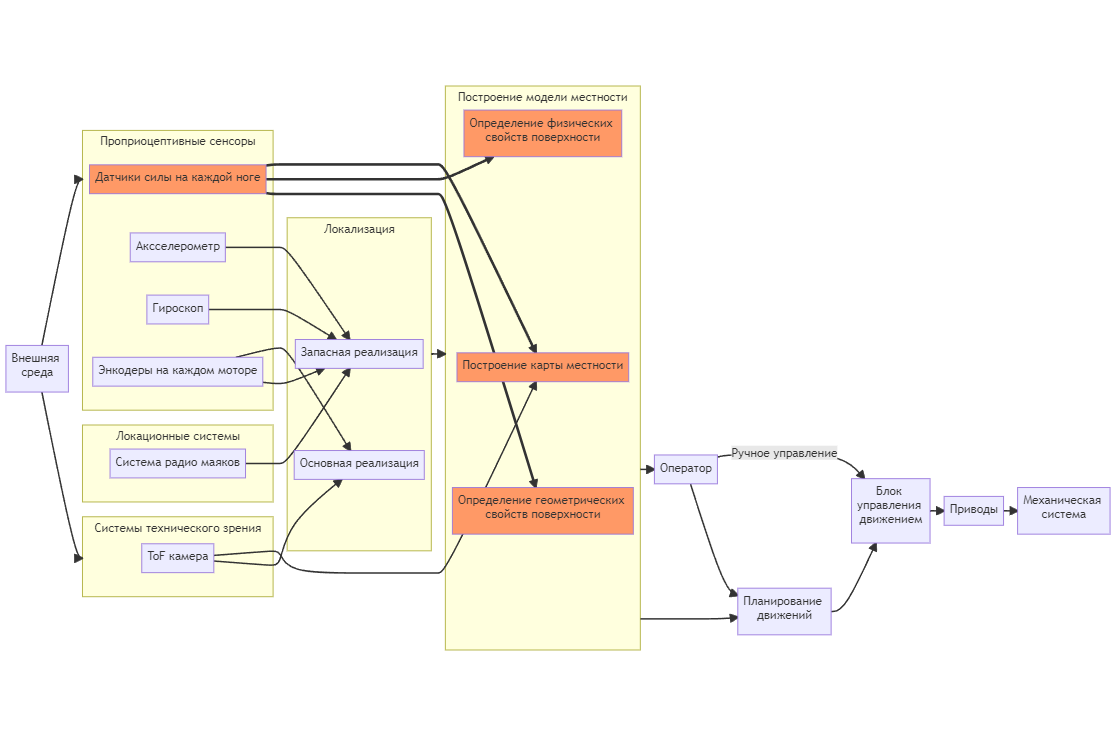
\includegraphics[height=10cm,width=1\textwidth,keepaspectratio]{diag_system.png}
    \caption{Структурная схема разрабатываемой системы}
    \label{fig:diag_system.png}
\end{figure}

Оранжевым цветом выделены те элементы, которые были разработаны и изучены, остальные --- взяты готовые решения. Жирными стрелками показаны те блоки, на которых сделан упор в диссертации.

В работе научная новизна представлена в блоках, связанных с очувствлением: датчики силы, построение карты местности, определение физических свойств объекта. Для улучшения текущих решений необходимо разбираться в самых современных алгоритмах и концептах, связанные с этой тематикой.


\section{Применимость системы}
Необходимо понимать возможности робототехнической системы. Следующая задачей является формализация условий ее применимости. Из полученных условий возможно определить конкретные существующие места, где такую систему возможно применить.

Как итог, был сделан вывод, что данная система может использоваться в узких пещерах, где не может пролезть человек. Шагающие машины обладают лучшей проходимостью, чем гусеничный или колесный тип движителя, поэтому его использования в местах, где есть большой перепад высот и нет возможности набирать высокую скорость из-за обилия препятствий обоснован. Датчики силы на основе Velostat являются самыми подходящими для разрабатываемой робототехнической системы по причине соотношения цены и точности. Для получения геометрической поверхности модифицируется алгоритм создания вогнутой оболочки с помощью триангуляции Делоне и alpha геометрии. Физические свойства поверхности определяются с помощью обучения стендовой установки на различных типах поверхности с использованием алгоритма SVM и kNN.           % Глава 1
\chapter{Оптимизация конструкции робота}\label{ch:ch2}

Вторая глава покрывает разработку объекта исследования, а именно решение задачи структурного синтеза и инженерную разработку прототипа.

\section{Задача структурного синтеза на основе критериев проходимости, детализации и пройденного пути}

Зная область применения робототехнической системы возможно оптимизировать ее механическую часть. Были выставлены следующие требования:
\begin{enumerate}
    \item иметь малые габариты, чтобы иметь возможность пролезать через щели в скальной породе и не застревать среди камней;
    \item обладать достаточной проходимостью по сыпучим грунтам;
    \item иметь возможность преодолевать малые водные преграды;
    \item мог взбираться на большие каменные уступы.
\end{enumerate}

\begin{figure}[H]
    \begin{subfigure}{0.9\textwidth}
        \centering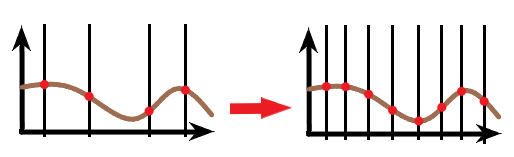
\includegraphics[height=6cm,width=1\textwidth,keepaspectratio]{f1.png}
        \caption{При увеличении количества ног увеличивается детализация картографируемой поверхности}
        \label{fig:f1.png}
    \end{subfigure}

    \begin{subfigure}{0.9\textwidth}
        \centering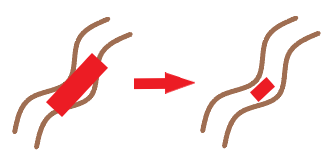
\includegraphics[height=6cm,width=1\textwidth,keepaspectratio]{f2.png}
        \caption{При увеличении количества ног, корпус робота увеличивается и он не может пройти часть препятствий}
        \label{fig:f2.png}
    \end{subfigure}

    \begin{subfigure}{0.9\textwidth}
        \centering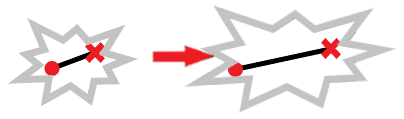
\includegraphics[height=6cm,width=1\textwidth,keepaspectratio]{f3.png}
        \caption{Изменение количества ног неявно влияет на проходимость системы}
        \label{fig:f3.png}
    \end{subfigure}

\caption{Критерии оптимизации конструкции робота}
\label{fig:opti_criteria}
\end{figure}
Изучая данные требования возможно заметить, что часть из них коррелируют друг с другом, а часть - антогонируют. Чем больше количество полученных точек на пройденной поверхности, тем выше будет детализация карты. Одним из способов увеличения детализации это увеличение количества ног у робота \pic{fig:f1.png}. С другой стороны, это увеличивает длину робота, а следовательно робот хуже сможет проходить узкие участки с обилием поворотов \pic{fig:f2.png}. Чем большее расстояние робот сможет пройти за одно и то же время, тем быстрее будет построена карта и робот меньше повлияет на окружающую среду при прочих равных условиях \pic{fig:f3.png}. 

Как итог возникает задача, которая не имеет одного лучшего решения. Следовательно, это мультикритериальная задача оптимизации.


Было решено, что цикловой движитель с одной степенью свободы в ноге лучше всего подходит для решения подобных задач.

Для цикловых движителей с одной степенью свободы в ноге вопрос о количестве ног не имеет однозначного решения. Поэтому необходимо провести структурный синтез, чтобы определить их количество. Данная задача решалась с помощью генетического алгоритма.

Генетический алгоритм это эвристический алгоритм поиска, используемый для решения задач оптимизации и моделирования путём случайного подбора, комбинирования и вариации искомых параметров с использованием механизмов, аналогичных естественному отбору в природе. Для решения задачи использовалась библиотека Deap и OpenAI.

Для создания подходящего робота, который может эффективно решать конкретные задачи, необходимо провести структурный синтез. Это означает, что оптимизируются такие характеристики робота, как количество ног, угол между ногами и т.д., используя алгоритмы оптимизации.

При оптимизации очень важно выбрать подходящую функцию пригодности. Иногда эта функция может быть явно выражена через аналитическую формулу: например, выражение общего материального объема робота как функции его геометрических параметров. Однако, в других случаях желаемая мера эффективности не может быть вычислена в явном виде и может быть получена только с помощью физического эксперимента или соответствующего моделирования. В данном случае важно максимизировать ходовые качества робота на различных сложных участках, и основным используемым показателем будет проходимость по местности. Генерируется семейство роботов, изменяя выбранные параметры конструкции робота, такие как количество ног.

Понятие сложности поверхности субъективно. Поэтому хорошей практикой ей генерация семейства проходимых поверхностей. Затем оценивается пригодность робота для ходьбы с помощью физической симуляции, во время которой робот будет проходить по местности. Также были получены параметризации различных генеративных моделей местности, чтобы было возможно на более позднем этапе исследовать влияние не только типа местности, но и параметров местности и, следовательно, на лучшие конструкции в зависимости от конкретной местности.

Для того чтобы направлять процесс поиска в пространстве возможных значений параметров, решено использовать модифицированный эволюционный алгоритм, который создает последовательные поколения конструкций с помощью соответствующих генетических операторов, играющих роль мутаций и скрещивания. После нескольких инициализаций и поколений были получены многообещающие результаты и полезные идеи, которые позволили создать конструкции, значительно улучшающие производительность, для достижения конечной цели - многоножек, способных преодолевать сложные участки местности.

\subsection{Математическая модель робота}
Исследуется механическая система, состоящая из твёрдых тел \eqref{eq:newton_euler}, движение которых описывается дифференциальными уравнениями вида:

\begin{align}
    \label{eq:newton_euler}
    M \dot{\vec{u}} = \vec{g} \\
    M = \begin{bmatrix}
    M_1 & \cdots  & 0 \\
    \vdots  & \ddots  & \vdots  \\ 
    0 & \cdots   & M_n 
    \end{bmatrix},\ M_i = \begin{bmatrix}
    m_i E_{3\times 3} & 0 \\ 
    0 & I_i 
    \end{bmatrix} \\
    \vec{u}_i^{\ T} = \begin{bmatrix}
        \vec{v}_i^{\ T} & \vec{\omega}_i^{\ T}
    \end{bmatrix} \\ 
    \vec{g}^{\ T} = \begin{bmatrix}
        \cdots \  \vec{F}_i^{\ T}, & (\vec{\tau}_i - \vec{\omega}_i \times I_i \vec{\omega}_i)^T\  \cdots 
    \end{bmatrix}
\end{align}
где, $M_i$~---~матрицы, содержащие массово-инерционные характеристики; $m_i$~---~масса тела; $I_i$~---~тензор инерции; $\vec{u_i}$~---~вектор обобщённых скоростей; $E$~---~единичная матрица; $\vec{g}$~---~вектор обобщённых сил; $\vec{v_i}$~---~вектор линейной скорости; $\vec{\omega_i}$~---~вектор угловой скорости; $\vec{F_i}$, $\vec{\tau_i}$~---~силы и моменты сил взаимодействия.

Тела, входящие в систему соединены между собой цилиндрическими шарнирами, которые описываются следующими связями и динамическими ограничениями:
\begin{align}
    \label{eq:kin_constr}
    \phi(q_{j_1},\ u_{j_1},\ \cdots,\ q_{j_k},\ u_{j_k},\ t) \geqslant  0 \\
    \vec{q}_i^{\ T} = \begin{bmatrix}
        \vec{x}_i^{\ T} & \vec{Q}_i^{\ T}
    \end{bmatrix} \\
    \dot{\vec{q}_i} = \begin{bmatrix}
    E_{3\times3} & 0\\ 
    0 & G(\vec{q}_i) 
    \end{bmatrix}\vec{u}_i  
\end{align}

\begin{align}
    \label{eq:phys_constr}
    \vec{g}_i = \tau_i^T \vec{z}_{i-1} -k\vec{v}_i \dot{\vec{q}_i} 
\end{align}
где через $\phi$ обозначена функция связи; $t$~---~время; $q_{j}$~---~вектор обобщенных координат, включающий в себя координаты центра масс $\vec{x_i}$ и кватернион $\vec{Q_i}$, описывающий ориентацию тела в пространстве; через $G(\vec{q}_i)$ обозначена матрица, вид которой зависит от выбранной системы координат и способа задания ориентации тела; $k$~---~ коэффициент вязкого трения в шарнире.

Контакт ног робота с опорной поверхностью \pic{fig:contact_interaction.png} описывается на базе модели сухого трения и выражатеся следующими уравнениями:

\begin{figure}[H]
    \centering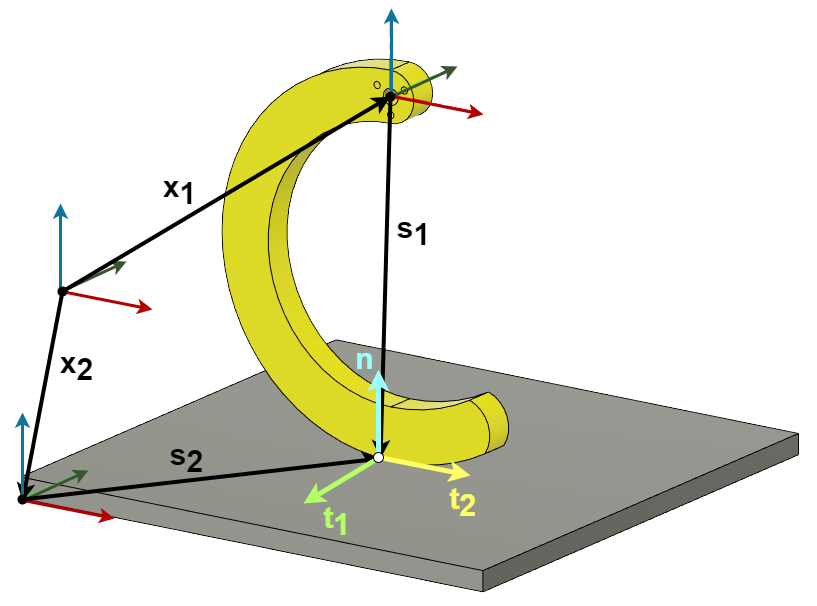
\includegraphics[height=9cm,width=1\textwidth,keepaspectratio]{images/contact_interaction.png}
    \caption{Описание переменных для модели взаимодействия опорной поверхности и ноги робота}
    \label{fig:contact_interaction.png}
\end{figure}

\begin{align}
    \label{eq:contact_inter}
    \phi_u(\vec{q}\ ) = g(\vec{q}\ ) \geqslant 0 \\ 
    g(\vec{q}\ ) = (\vec{x}_1 + \vec{s}_1 - \vec{x}_2 - \vec{s}_2) \cdot \vec{n} \\
    \frac{d }{d t}\phi_u(\vec{q}\ ) \approx \begin{bmatrix}
        \vec{n}^{\ T} & (\vec{s}_1 \times \vec{n})^T & -\vec{n}^{\ T} & (-\vec{s}_2 \times \vec{n})^T
    \end{bmatrix} \begin{bmatrix}
        \vec{v}_1\\ 
    \vec{\omega}_1\\ 
    \vec{v}_2\\
    \vec{\omega}_2\\
    \end{bmatrix}
\end{align} 

\begin{align}
    \label{eq:ground_inter}
\left\{\begin{matrix*}[l]
\mu f_n \geqslant \sqrt{f_1^2 + f_2^2}\\ 
\left\lVert \vec{v_t}\right\rVert (\mu f_n - \sqrt{f_1^2 + f_2^2}) = 0\\
\dfrac{\vec{f_t}}{\left\lVert \vec{f_t}\right\rVert } = - \dfrac{\vec{v_t}}{\left\lVert \vec{v_t}\right\rVert }
\end{matrix*}\right.
\end{align}
где, $\phi_u(\vec{q})$~---~функция связи; $ \mu $~---~ коэффициент трения между ногой и опорной поверхностью;  радиус-векторы $\vec{x}_{1,2},\ \vec{s}_{1,2}$ и орты координатных осей $\vec{t}_{1,2}, \vec{n}$ показаны на рисунке \pic{fig:contact_interaction.png}; $ f_{1,2} $~---~значения сил трения вдоль осей $t_{1,2}$ соответственно.

\subsection{Представление робота}

Геометрическая модель робота представлена в виде трехмерного параллелепипеда. Количество движителей по каждому из бортов обозначается через $\gamma$. Разность фаз между соседними движителями обозначается через  $\alpha$ \pic{fig:best_gen_robot.jpg}.

\begin{figure}[H]
    \centering
    \begin{tikzpicture}
        % Include the image in a node
        \node [above right, inner sep=0] (image) at (0,0)
        {\centering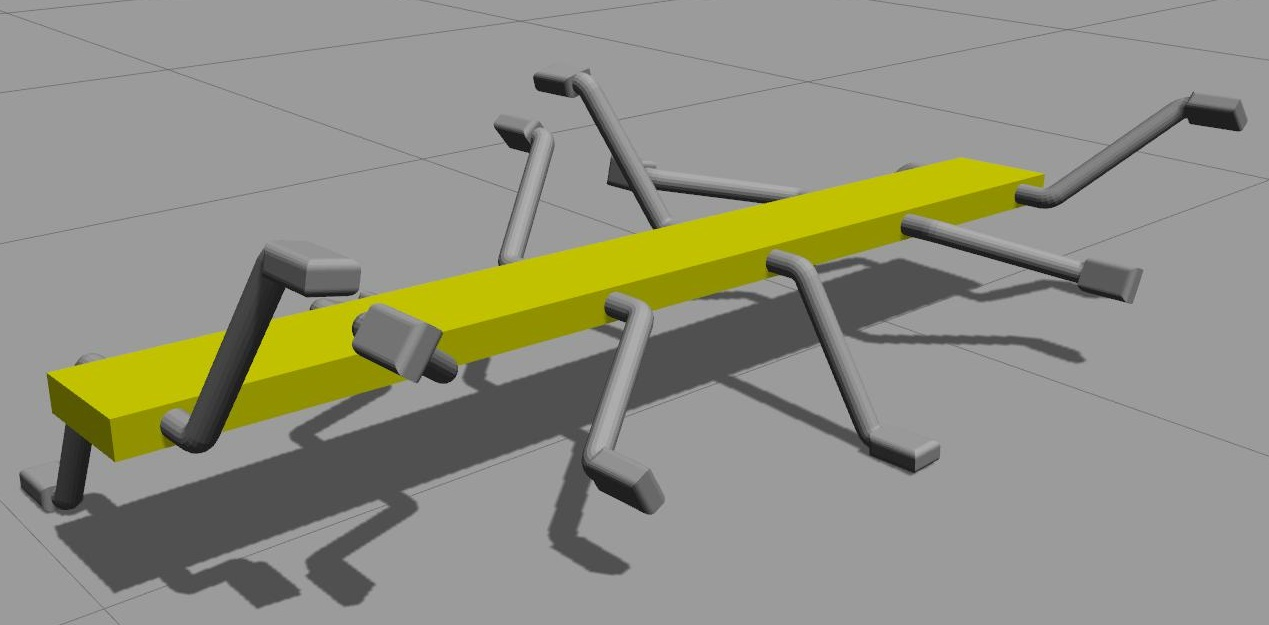
\includegraphics[height=10cm,width=0.8\textwidth,keepaspectratio]{best_gen_robot.jpg}};
        % Create scope with normalized axes
        \begin{scope}[
                x={($ 0.1*(image.south east)$)},
                y={($ 0.1*(image.north west)$)}]
            % Labels
            \draw [green, very thick,
                decorate,
                decoration = {brace,
                        raise=5pt,
                        amplitude=5pt,
                        aspect=0.5}] (1.4,3.6) --  (8.1,6.8)
            node[rounded corners=3pt, pos=0.5,above left =14pt,black,fill=white]{\tiny $(\gamma - 1) h_{\text{leg}}\sin(\alpha)$};

            \draw[stealth-, very thick,green] (9.5,7.8) -- (7.8,1.94);
            \draw[stealth-, very thick,green] (1.5,2.8) -- (7,1)
            node[rounded corners=3pt,right,black,fill=white]{\tiny $\gamma = 6$};

            \draw[thin,green] (6.7,4) -- (5.75,9);
            \draw[thin,green] (4.85,3.5) -- (5.75,9);
            \draw[thin,green,stealth-stealth] (6.32,6) arc (-79.2:-99.2:3) node [rounded corners=3pt,below = 2pt,black,fill=white, midway] {\tiny $\alpha$};
        \end{scope}
    \end{tikzpicture}
    \caption{Схема модели робота для генетического алгоритма}
    \label{fig:best_gen_robot.jpg}
\end{figure}

Эту задачу можно сформулировать как мультикритериальную задачу оптимизации, где необходимо максимизировать дистанцию, пройденную за фиксированное время, и минимизировать длину робота \eqref{eq:second}. Параметрами индивида являлись $\gamma$ и $\alpha$.

\begin{align}
    \label{eq:second}
    F \rightarrow max = \beta \left( {\omega}_{1} \cdot \overbrace{\delta}^{\text{Distance}} + {\omega}_{2} \cdot \overbrace{\frac{1}{(\gamma - 1) h_{\text{leg}}\sin(\alpha)}}^{\text{Simplified body length}}\right) + \\ \nonumber + (1 - \beta) {\delta}^{{\omega}_{1}} {\left( \frac{1}{(\gamma - 1)h_{\text{leg}}\sin(\alpha)}\right)}^{{\omega}_{2}}
\end{align}
где \nom{$\delta$}{пройденная дистанция}, \nom{$\beta$}{адаптивный параметр}, \nom{${\omega}_{1,2} \in  [ 0..1 ] $}{весовые коэффициенты}.


Модель робота должна быть реализована в формате URDF. Это язык разметки формата XML для представления модели робота. Но это старый формат, и когда модель импортируется в Gazebo, URDF преобразуется в формат SDF. Это важно, потому что некоторые функции не реализованы в чистом URDF. В нашем случае это шарнир коробки передач. Но можно вставить код в формат SDF, и он будет работать правильно.

\subsection{Генерирование местности, по которой будет проходить робот}
Прежде чем говорить о генерировании местности, необходимо обосновать данное решение. Глобальная задача это оценить сложность рельефа. Основными найденными подходами к оценке рельефа являются.
\begin{enumerate} 
    \item Анализ множества физических свойств поверхностей, таких как ковер или линолеум, с точки зрения максимальной скорости, мощности и других параметров робота при их прохождении \cite{Altendorfer2001}.
    \item Построение конкретной местности, которая является достаточно сложной в субъективном плане. В задании Rough Terrain Task в DARPA's Virtual Robotics Challenge используется этот подход. Таким образом тестировался робот ATLAS \cite{feng_Optimizationbased_2015} \pic{fig:terrain_assesment/c2_paper.jpg}.
          
          \begin{figure}[H]
              \centering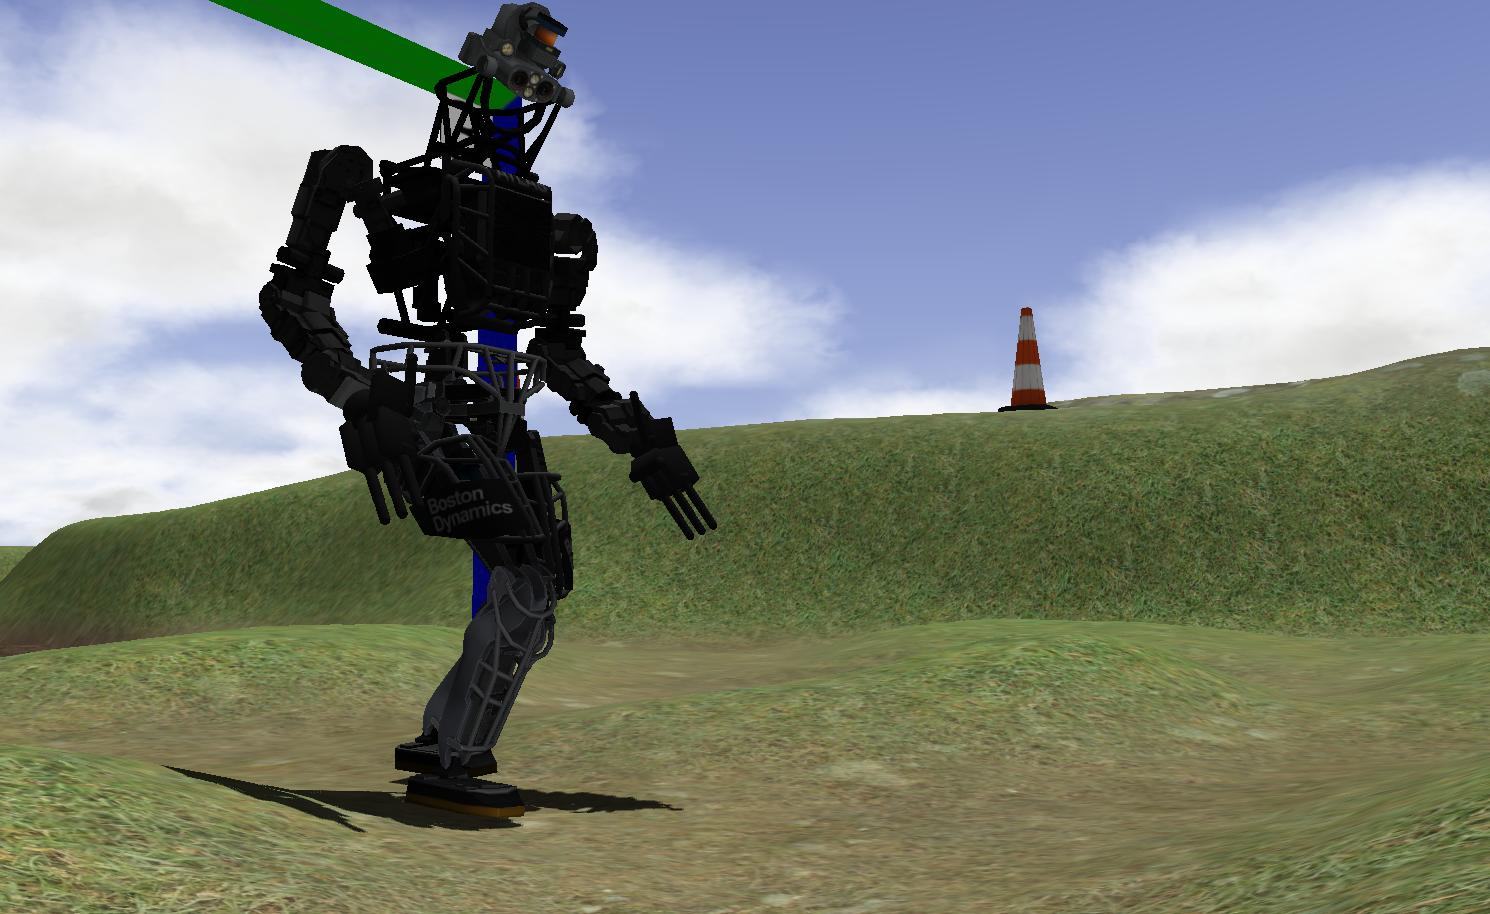
\includegraphics[height=6cm,width=1\textwidth,keepaspectratio]{terrain_assesment/c2_paper.jpg}
              \caption{Задание на пересеченной местности в конкурсе виртуальной робототехники DARPA}
              \label{fig:terrain_assesment/c2_paper.jpg}
          \end{figure}
          
    \item Оценка местности в соответствии с возможностями робота. Она основывается на максимальном перепаде высот, который может преодолеть робот. Если робот не может его преодолеть, значит, местность неудовлетворительная \cite{hung_Advanced_2004,Howard2000} \pic{fig:terrain_assesment/c3_paper.png}.
          
          \begin{figure}[H]
              \centering\includegraphics[height=6cm,width=1\textwidth,keepaspectratio]{terrain_assesment/c3_paper.png}
              \caption{Пример карт местности: карта опасности местности и карта достоверности местности}
              \label{fig:terrain_assesment/c3_paper.png}
          \end{figure}

    \item Оценка по карте с использованием ряда анализируемых параметров, таких как дисперсия, дальность, тип почвенно-растительного покрова, количество треугольных граней и так далее \cite{hung_Advanced_2004}.
    \item Получение искусственных поверхностей на основе параметров генерации. Первая версия этой идеи была связана с получением жестких ландшафтов с квадратной сеткой, где каждая ячейка имеет некоторую высоту \cite{sancho-pradel_Survey_2010} \pic{fig:terrain_assesment/c1_paper.png}.
          
          \begin{figure}[H]
              \centering\includegraphics[height=8cm,width=1\textwidth,keepaspectratio]{terrain_assesment/c1_paper.png}
              \caption{Рельеф с параметризованными ячейками}
              \label{fig:terrain_assesment/c1_paper.png}
          \end{figure}
\end{enumerate}

После тщательного рассмотрения было решено, что последний подход с некоторыми модификациями и расширениями лучше всего подходит для нашей задачи.

Параметры местности, которые могут быть изменены, следующие:
\begin{itemize}
\item номер ширины и длины клетки;
\item диапазон высоты клетки начало и конец;
\item ширина и длина клетки;
\item 2(3) измерения местности (рис.~\ref{fig:terrain_1});
\item параметр распределения (рис.~\ref{fig:terrain_2}).
\end{itemize}

Для выбора высоты клеток были проведены эксперименты.
Существует 3 диапазона, определяющих свойства местности, которые изображены ниже (рис.~\ref{fig:range}).

\begin{figure}[H]
\centering\includegraphics[width=0.5\textwidth]{from_master/ranges}\\
\caption{Три диапазона для оценки рельефа местности}
\label{fig:range}
\end{figure}

Для каждого диапазона было сгенерировано 20 местностей и 50 роботов. Каждый робот пытается пройти все местности. У робота есть 4 секунды на попытку. Успешные попытки засчитывались. Результаты можно увидеть в таблице \ref{tabular:ranges}.

\begin{table}[H]
\caption{Процентное соотношение между диапазонами и успешными попытками}
\label{tabular:ranges}
\centering
\begin{tabular}{c|c}
 \textbf{Диапазон} & \textbf{Процент успешных попыток}\\
 \hline
0.00 -- 0.08 & 99.7 \\ 
0.08 -- 0.16 & 79.7 \\
0.16 -- 0.195 & 47.3 \\
\end{tabular}
\end{table}


Таким образом, было решено, что второй и первый диапазоны (0.00 - 0.16) будут использоваться в алгоритме оптимизации.

В информатике генетические алгоритмы - это адаптивные эвристические алгоритмы поиска, основанные на эволюционных концепциях. Они представляют собой интеллектуальную параллельную эксплуатацию пространства проектирования и могут быть использованы для решения проблем оптимизации, не обязательно оптимизируя, но часто получая близкие к оптимальным решения. 

Реализация генетического алгоритма основана на библиотеках Deap  и OpenAI-ES \cite{DEAP_JMLR2012,salimans_Evolution_2017}.

Генетический код особи содержит 3 основных гена: количество ног, угол между двумя соседними ногами и волновое смещение между сторонами, а также 1 дополнительный ген~--- пройденная дистанция, который зависит от других генов и поэтому не участвует в процедурах скрещивания и мутации. 

Алгоритм заключается в следующем. После случайной генерации начальной популяции, популяция эволюционирует с помощью трех операторов: селекции, основанного на повышенной вероятности выживания сильнейшего; скрещивания, который представляет собой спаривание между особями и мутации, которая вносит случайные изменения в значения генов отдельных особей.

Процедура селекции, реализующая турнирный подход, была взята из библиотеки Deap без изменений. 

Были написаны собственные реализации скрещивания и мутации:
\begin{enumerate}
\item Для скрещивания используется общая функция с некоторыми дополнениями. Каждая особь имеет 4 гена, но четвертый ген (расстояние) зависит от других генов. Поэтому функция скрещивания должна работать только с первыми тремя характеристиками.

\item Мутация: Аналогично скрещиванию, используется только 3 поля. Модель робота имеет ограничения, например по максимальной длине, поэтому с некоторой заданной вероятностью каждая из характеристик может быть изменена в определенном интервале. Допускается осуществление с одной и той же особью нескольких мутаций, но с каждым разом вероятность мутации уменьшается. 
\end{enumerate}

Этот псевдокод дает высокоуровневое описание всего алгоритма.

\begin{algorithm}[H]
\caption{Верхеуровневый генетический алгоритм\label{high_level}}
% \begin{small}
\KwIn{$\alpha$ -- количество поколений, $\beta$ -- количество индивидов, $\gamma$ -- количество территорий}
\KwOut{Хорошие параметры для робота}
\Begin{
Генерация семейства поверхностей\;
случайная генерация первого поколения индивидов\;
\For{$i = 0$ \KwTo $\alpha$}{
\For{$j = 0$ \KwTo $\beta$}{
$distance = 0$\;
\For{$k = 0$ \KwTo $\gamma$}{
Начало симуляции\;
$distance += cur\_distance$\;
}
$avg\_distance = distance / \gamma$\;
высчитывание фитнес функции\;
}
выбор лучших родителей\;
скрещивание выбранных родителей\;
мутация генов\;
}
}
% \end{small}
\end{algorithm}

Было проведено два эксперимента. В первом эксперименте искались лучшие параметры робота для территории T1. Во втором эксперименте рассматривалась зависимость от разных типов ландшафтов при меньшем количестве индвидов. Весовые коэффициенты $\omega_1,\ \omega_2$ варьировались, но здесь и далее приведены данные, полученные при $\omega_1 = 0.6,\ \omega_2 = 0.4$. 

\begin{figure}[H]
    \begin{subfigure}{0.33\textwidth}
    \centering\includegraphics[width=0.8\textwidth]{terrain_1} 
    \caption{T1: 3D-боксы с равномерным распределением высоты}
    \label{fig:terrain_1}
    \end{subfigure}
    \begin{subfigure}{0.33\textwidth}
    \centering\includegraphics[width=0.8\textwidth]{terrain_2} 
    \caption{T2: 2D-полосы с гауссовой функциональной высотой}
    \label{fig:terrain_2}
    \end{subfigure}
    \begin{subfigure}{0.33\textwidth}
    \centering\includegraphics[width=0.8\textwidth]{terrain_3}
    \caption{T3: 2D-полосы с распределением высоты по гауссовской функции)}
    \label{fig:terrain_3}
    \end{subfigure}
     
    \caption{Примеры сгенерированных территорий}
    \label{fig:terrains}
\end{figure}

\begin{figure}[H]
    \centering\includegraphics[width=0.6\textwidth]{from_master/best_robot}\\
    \caption{Робот с результирующими результатами}
    \label{fig:best_robot}
    \end{figure}
    \begin{figure}[H]
    \centering\includegraphics[width=0.6\textwidth]{from_master/best_robot_200_plot}\\
    \caption{Среднее значение фитнес-функции $\pm$ std на поколение
    Минимальное и максимальное значения фитнес-функции на поколение}
    \label{fig:plot4}
    \end{figure}
    
    Весовые коэффициенты настраивались в зависимости от выбора приоритета. Невзирая на выбранные коэффициенты, оптимальным набор ног начинался с 8 и заканчивался 14. Это объясняется критерием статического равновесия, который, как оказалось, увеличивает проходимость механизма. В данном случае 4 ноги всегда будут касаться пола. 
    
    Первый эксперимент: каждый робот проходил 10 разных ландшафтов по 9 секунд каждую. Второй эксперимент: она имеет те же параметры, что и первая фаза, но с измененным размером популяции. 
    
    В соответствии с таблицей \ref{tabular:Table2} (весовые коэффициенты равны 0.6 и 0.4 соответственно) видна сходимость в параметрах. Видео прохождения препятствия лучшим индивидом \quad
    \qrcode[height=1.5cm]{https://youtu.be/DcovvkTZgsg}


\begin{table}[ht]
\centering
\caption{Зависимость между статистикой целевой функции и типами поверхности}
\label{tabular:Table2}
\begin{tabular}{c|c|c|c}
    \rowcolor{Gray}
\textbf{Территория, популяция} & \textbf{Параметры} & \textbf{AVG} & \textbf{STD}\\
\hline
\textbf{T1 \pic{fig:terrain_1}, 110} & (6, 72) & 2.38 & 0.34
\\
\rowcolor{LightGray}
\textbf{T2 \pic{fig:terrain_2}, 55}& (5, 68) & 1.95 & 0.35
\\
\textbf{T3 \pic{fig:terrain_3}, 55} & (6, 77) &  2.08 & 0.33 \\
\hline
\end{tabular}
\end{table}

Одним из основных результатов исследования, полученных при варьировании значений весовых коэффициентов $\omega$ является зависимость между количеством ног и пройденной дистанцией \pic{fig:box_plot_structural_synthesis.png}, которая показала наличие локального оптимума при количестве ног у робота в диапазоне от 8 до 14. 

\begin{figure}[H]
    \centering\includegraphics[height=10cm,width=1\textwidth,keepaspectratio]{images/box_plot_structural_synthesis.png}
    \caption{Зависимость между количеством ног и пройденной дистанцией}
    \label{fig:box_plot_structural_synthesis.png}
\end{figure}

Автор полагает, что этот факт может быть объяснён следующими соображениями. С одной стороны, слишком много ног значительно удлиняет корпус робота, что снижает его профильную проходимость за счёт того, что робот с большей вероятностью может задеть выступы при движении. С другой стороны при слишком малом количестве ног происходит потеря статической устойчивости робота. Поскольку для гарантированного обеспечения статической устойчивости необходимо обеспечить контакт не менее, чем 4 ног с опорной поверхностью в каждый момент времени, то естественным ограничением является 8 ног у робота.


\section{Задача оптимизации колебаний робота при походке}
Несмотря на то, что каждая нога робота может двигаться независимо, что позволяет получать абсолютно разные походки, возможно определить оптимальный угол между ногами робота при движении по плоскости. Под оптимальностью подразумевается максимальный клиренс и минимальные колебания системы. Клиренс это расстояние от корпуса робота, до опорной поверхности. Это позволит быстро преодолевать прямые участки с минимальным риском для оборудования, находящегося в роботе.

Задача целевой функции --- максимизировать положение $Z$ и минимизировать $STD$. Одновременно необходимо сделать минимальным $RMS$ и $STD$ углов в обоих направлениях (крен и тангаж). Важным моментом является и направление движения.

Целевая функция имеет следующий вид:
\begin{align}
    \label{eq:objective}
    F = \sum\limits_{i=1}^4 \omega_{i} \cdot (\frac{1}{\omega_{z1}Z_{rms}^i - \omega_{z2}Z_{std}^i}  + ( \omega_{p1}\alpha_{rms}^i + \omega_{p2}\alpha_{std}^i) + \nonumber \\\ + (\omega_{r1}\beta_{rms}^i + \omega_{r2}\beta_{std}^i)) \rightarrow min
\end{align}
где надпись \nom{$i =\{1,2,3,4\}$}{среднее значение a, которое принимается из 1 - движение вперед, 2 - движение влево, 3 - движение вправо, 4 - вращение}; \nom{$Z$}{положение по оси Z}; \nom{$\alpha, \beta$}{значения ориентации по крену и шагу}; \nom{$\omega_{i}$}{весовой коэффициент для каждого направления}, \nom{${\omega}_{z,roll,pitch}$}{весовые коэффициенты}.

Возможно решить задачу полным перебором, так как надо проверить 36 углов ~$\cdot$ 4 направления ~$\cdot$ 100 экспериментов для каждого направления ~$\cdot$ 144 шага в каждом.

Есть пример, который описывает два возможных движения: вперед и скольжение. Результаты о положении почти одинаковы для обоих типов.

\begin{figure}[H]
\begin{subfigure}{1\textwidth}
\centering\includegraphics[width=0.9\textwidth]{from_master/forwardBestMean} 
\caption{Среднее значение из данных о положении для обоих типов движения}
\label{fig:forwardBestMean}
\end{subfigure}

\begin{subfigure}{1\textwidth}
\centering\includegraphics[width=0.9\textwidth]{from_master/forwardBestSTD} 
\caption{STD из данных о положении для обоих типов движения}
\label{fig:forwardBestSTD}
\end{subfigure}
 
\caption{Данные о положении для обоих типов движения}
\label{fig:forwardPosion}
\end{figure}

\begin{figure}[H]
\centering\includegraphics[width=0.9\textwidth]{from_master/forwardBestRMSrot} 
\caption{RMS из данных об ориентации для типа движения вперед}
\label{fig:forwardBestRMSrot}
\end{figure}

\begin{figure}[H]
\centering\includegraphics[width=0.9\textwidth]{from_master/forwardBestSTDRot} 
\caption{STD из данных об ориентации для типа движения вперед}
\label{fig:forwardBestSTDRot}
\end{figure}

\begin{figure}[H]
\begin{subfigure}{1\textwidth}
\centering\includegraphics[width=0.9\textwidth]{from_master/slideBestRMSrot} 
\caption{RMS из данных об ориентации для типа движения вбок}
\label{fig:slideBestRMSrot}
\end{subfigure}

\begin{subfigure}{1\textwidth}
\centering\includegraphics[width=0.9\textwidth]{from_master/slideBestSTDRot} 
\caption{STD из данных об ориентации для типа движения вбок}
\label{fig:slideBestSTDRot}
\end{subfigure}
 
\caption{из данных об ориентации для типа движения вбок}
\label{fig:slideOrientation}
\end{figure}

В результате работы получен угол между ногами равный 120 градусам. Это можно объяснить, потому что это периодическая функция, а обычно этот тип функций дает подходящие результаты.

\section{Оптимизация конструкции робота для прохождения узких участков}

В первом пункте требований к движителю (начало главы) стоит требование, чтобы робот не застревал при поворотах. Проблема застревания решается с помощью изменения угла между ногой и корпусом робота.

Возможность двигаться во все направления без смены ориентации сильно повышает проходимость робототехнической системы во многих случаях. Классическая компоновка многоногого шагающего робота с одной степенью свободы в ноге не позволяет перемещаться таким образом. Но если воспользоваться концептом, который используется в всенаправленных колесах, то шагающий робот с одной степенью свободы в ноге сможет перемещаться всенаправленно без смены ориентации.

\begin{figure}[H]
    \centering\includegraphics[height=10cm,width=1\textwidth,keepaspectratio]{omni_rot.png}
    \caption{Векторное представление сил в классическом и всенаправленном состоянии}
    \label{fig:omnidirection}
\end{figure}

На рисунке \ref{fig:omnidirection} представлена иллюстрация данной концепции: для того, чтобы робот двигался во всех направлениях, необходимо разбить ноги на группы, чтобы получилось 4 группы A-D.

Если сравнивать с классической компоновкой роботов (угол между корпусом робота и осью вала привода ноги равен 90 градусов), то вектор внешних сил будет таким, как на левой части рис. \ref{fig:omnidirection}. Стрелка в центре робота — суперпозиция всех сил. Если изменить угол оси привода ноги в соответствии с предлагаемой концепцией, то возможно получить значения суперпозиции сил, представленные на рис. \ref{fig:omnidirection} в центре. То есть, чтобы переместить корпус робота направо, группы А и D должны вращать ноги в одну сторону, а группы C и B — в противоположную. Правая часть рисунка иллюстрирует расположение групп ног на исследуемом роботе. 

\section{Разработанные концепции робота}

В рамках исследования было разработано четыре концепции робота СтриРус. В таблице \ref{tabular:robot_comparison_body} в строке недостатки объясняются основные причины перехода из одной итерации к другой. Концептуально было замечено, что высота ноги и наличие сегмента разительно влияет на проходимость конструкции. \quad \qrcode[height=1.5cm]{https://youtu.be/EQ6oGZVDpoc}

\begin{figure}[H]
    \centerfloat{
        \hfill
        \subcaptionbox[List-of-Figures entry]{Первая итерация\label{fig:strirus_0}}{%
            \includegraphics[width=0.49\linewidth]{strirus_0.png}}
        \hfill
        \subcaptionbox[List-of-Figures entry]{Вторая итерация \label{fig:strirus_1}}{%
            \includegraphics[width=0.49\linewidth]{strirus_1.png}}

        \hfill
        \subcaptionbox{Третья итерация\label{fig:strirus_2}}{%
        \includegraphics[width=0.49\linewidth]{strirus_2.jpg}}
        \hfill
        \subcaptionbox{Третья итерация, улучшенная\label{fig:strirus_3}}{%
        \includegraphics[width=0.49\linewidth]{strirus_3.JPG}}
        \hfill

        \subcaptionbox{Четвертая итерация\label{fig:strirus_4}}{%
        \includegraphics[width=0.9\linewidth]{strirus_4.png}}
    }
    % \legend{Подрисуночный текст, описывающий обозначения, например. Согласно
    %     ГОСТ 2.105, пункт 4.3.1, располагается перед наименованием рисунка.}
    \caption{Итерации робота СтриРуса}\label{fig:striruses}
  \end{figure}

  \begin{table}[H]
    \caption{Сравнение итераций робота}
    \label{tabular:robot_comparison_body}
    % \begin{center}
    \small
    \begin{tabular}{p{2cm}|p{2cm}|p{2cm}|p{2cm}|p{2cm}|p{2cm}}
    \toprule
    \toprule
    % \rowcolor{Gray}
     Итерация & 1 \pic{fig:strirus_0}  & 2 \pic{fig:strirus_1} &  3 \pic{fig:strirus_2} & 3+ \pic{fig:strirus_3} & 4 \pic{fig:strirus_4} \\
     \hline
     Кол-во ног & 54 & 12 & 12 & 6 & 10 \\ 
    %   \rowcolor{lightgray}
     \makecell[l]{Кол-во \\ сегментов} & 1 & 2 & 2 & 1 & 2 \\
     \makecell[l]{Тип \\ соединения} & --- & Тангаж & \makecell[l]{Тангаж,\\ рыскание} & --- & Тангаж \\
    %  \rowcolor{lightgray}
     Отн. угол телом -- нога, градусы & 0 & 0--45 & 0, 15, 30, 45 & 0 & 0, 15 \\
     \makecell[l]{Высота \\ ноги, мм} & 54 & 60 & 60 & 90 & 170 \\
     \hline
     Особенности & Волноход & Механизм, который позволяет непрерывно изменять отн. угол & Двухстепенной узел, соединяющий сегменты & Большие ноги & Гигантские ноги  \\
    %  \rowcolor{lightgray}
    \hline
     Недостатки & Невозможно установить сенсоры на ноги. Много подвижных частей & Слишком сложный механизм, изменяющий отн. угол & Мал. ноги. Избыточная вторая степень свободы в соединительном узле & 1 сегмент. Маленькие ноги & --- \\
    \bottomrule
    \bottomrule
    \end{tabular}
    % \end{center}
    \end{table}

Как итог, был разработан 10 ногий двух сегментный робот СтриРус. 10 ног было выбрано на основе результатов, полученных во время решения мультикритериальной задачи оптимизации с помощью генетического алгоритма.

Результируя вышесказанное, получив паретто решение параметрической задачи оптимизации на основе критериев проходимости,  детализации и пройденного пути было выбрано решение с 10ью ногами робота. Оптимальным углом между ногами робота при движении по плоскости оказался 120 градусов. А идея по всенаправленному движению шагающего робота без смены ориентации, основанная на концепте всенаправленного колеса нашла свое подтверждение.



           % Глава 2
\chapter{Разработка и исследование преобразователя силы на основе Velostat}\label{ch:ch3}

Третья глава содержит описание этапов разработки и исследования пьезорезистивного тактильного преобразователя силы на основе материала Velostat. Тактильное очувствление является основным способом получения информации о геометрии и физических свойствах опорной поверхности по которой движется робот в условиях отсутствия видимости. Именно для шагающих аппаратов, в отличие от колёсных и гусеничных, такой способ является актуальным, поскольку ноги робота используются одновременно и как движители, и как устройства для ощупывания поверхности. В главе обосновано применения преобразователя силы на основе полимерного материала Velostat, представлены экспериментальные исследования работы преобразователя при площади нагрузки меньше
размеров самого преобразователя, что имитирует условия контакта ног шагающего робота с жесткой опорной
поверхностью, по результатам экспериментальных исследований показано при каких условиях характеристики преобразователя удовлетворяют требованиям к системе тактильного восприятия шагающего робота.

Среди возможных способов определения силы реакции опоры наиболее целесообразным представляется её измерение с помощью датчиков силы, расположенных непосредственно в зоне контакта ноги с опорной поверхностью. Среди доступных датчиков такого типа большинство обладают излишней чувствительностью и точностью, а также имеют очень высокую стоимость, что делает их применение неоправданным для использования в роботах, предназначенных для изучения труднодоступных мест, в которых высока вероятность потери робота. В связи с этим, предложено использовать преобразователь силы на базе материала Velostat. Первоначально Velostat был разработан как упаковочный материал, изготовленный из полимерной пленки (полиолефины), пропитанной сажей для придания ей электропроводности. Свойство изменять свое сопротивление при изгибе или давлении сделало материал популярным решением для изготовления недорогих
датчиков давления [120]. Такой датчик позволяет решить проблемы классификации местности и создания карт на биомиметическом многоногом роботе StriRus. Velostat обладает вязкоупругим поведением, а также свойствами квантового туннелирования и предварительной локализации, что существенно влияет на отклик датчика. Но при исследовании разработанного преобразователя, была замечена зависимость в результатах показания преобразователя при разных площадях касаемой поверхности и рабочей области сенсора. Эту зависимость необходимо формализовать.

Система из нескольких датчиков усилия, расположенных на опорной поверхности ноги робота позволяет определить величину и точку приложения силы реакции опоры. В совокупности с показаниями датчиков тока, определяющих нагрузку на двигателях, датчиков поворота ног, определяющих конфигурацию шагающего робота, а также инерциальных датчиков, определяющих ускорения корпуса робота и, соответственно, изменение его скорости, положения и ориентации, это потенциально даёт необходимую информацию как для определения геометрической формы, так и некоторых физических свойств поверхности, по которой движется робот.

В мобильных роботах широко используются сенсорные системы, которые включают в себя инерциальные измерительные приборы (IMU), датчики тока двигателей, датчики силы, звуковые датчики, системы технического зрения и другие оптические сенсоры \cite{libby_using_2012,ojeda_terrain_2006,peters_analysis_2006}. Однако, для решения указанных задач в условиях плохой видимости, оптические системы становятся неработоспособны, и на первый план выходит использование датчиков силы. В обнаружении формы поверхности. Существует класс роботов (RHEX, Strirus), которые обладают такими параметрами.

Как было отмечено в предыдущих разделах, наиболее перспективным является применение разрабатываемого шагающего робота в пещерах, поверхность которой имеет неровности и  состоит из твердых и скользких поверхностей, ходовых грунтов. Для работы в таких местах робот должен получать информацию о физических свойствах местности. Эта информация оказывает существенное влияние на эффективность и стратегии локомоции. Например, на зернистой или травянистой местности взаимодействие между ногами и землей может привести к резкому рассеиванию энергии из-за трения. Это происходит из-за деформации поверхности ногами. Знание этой информации о взаимодействии ноги с землей может быть использовано для управления адаптацией.

Имея подробную информацию о взаимодействии ноги-земля, возможно решить множество задач, таких как идентификация местности \cite{wuIntegratedGroundReaction2016, walasTerrainClassificationLocomotion2016, mrva_feature_2015, dallaire_learning_2015}, управление походкой на основе рельефа местности \cite{wuTactileSensingTerrainBased2020, weingarten_automated_2004}, анализ устойчивости и SLAM \cite{odenthal_nonlinear_1999, peters_analysis_2006, Altendorfer2001}. Решение этих задач позволяет значительно повысить проходимость и возможности исследования мобильных роботов.


Существует несколько типов датчиков, которые могут измерять контактные силы и распределение давления. Это могут быть оптические, пьезорезистивные, пьезоэлектрические, магнитные, емкостные, на основе оптических волокон \cite{howe_dynamic_1993}. Промышленные датчики момента силы (F/T) широко распространены на гуманоидах (Atlas, Fedor) или четвероногих (Spot, AnyMal). Однако они слишком велики для небольших роботов, таких как RHEX, WHEGS или StriRus \cite{saranli_design_2000,schroerComparingCockroachWhegs2004, bulichevConceptDevelopmentBiomimetic2018}. Та же проблема применима к оптическим и магнитным датчикам. Емкостные датчики требуют высокой точности изготовления. В свою очередь, пьезорезистивные датчики имеют маленькие размеры, могут быть размещены практически на любой поверхности, имеют низкую стоимость и не требовательны к условиям эксплуатации.

Самый популярный тип пьезорезистивного датчика - тензодатчик. Он может быть установлен на ногах робота, но это решение требует наличия цепей формирования сигнала и создает трудности при прокладке проводов между постоянно вращающимися ногами и корпусом робота \cite{wuTactileSensingTerrainBased2020}. Другой способ - использовать пьезорезистивные датчики на основе проводящих волокон или полимеров. Они недорогие, очень гибкие и компактные. К сожалению, одной из распространенных проблем является значительный гистерезис. Было решено использовать Velostat (Linqstat)\cite{vehecFlexibleResistiveSensor2020} в качестве промежуточного слоя для резистивного датчика.

Velostat --- это вязкоупругое проводящее волокно. Вязкие материалы, такие как медь, при сопротивлении сдвигаются и натягиваются линейно во время напряжения. Упругие материалы тянутся во время растягивания и быстро возвращаются в обратное состояние, когда уходит напряжение. проявляются свойства обоих типов, что, по сути, приводит к постепенному  изменению напряжения в материале в зависимости от времени. Это резко влияет на отклик датчика.
Вязкоупругое поведение материала является высоко нелинейным, что влияет на получаемые данные с сенсора.

На основе данного материала был разработан и изготовлен пьезорезистивный датчик, где материал Velostat \pic{fig:velostat_sensor.jpg} является промежуточным слоем для датчика \pic{fig:simplest_sensor.jpg}. 

Для использования такого датчика необходимо оценить его поведение. Например, выяснено, что если приложить одинаковую точечную силу в разных точках датчика, результат измерений будет значительно отличаться. Чтобы понять, как с этим работать, нужно сформулировать и смоделировать сценарии использования.

\begin{figure}[H]
    \begin{subfigure}[t]{0.9\textwidth}
        \centering\includegraphics[height=8cm,width=1\textwidth,keepaspectratio]{velostat_sensor.jpg}
        \caption{Материал Velostat}
        \label{fig:velostat_sensor.jpg}
    \end{subfigure}

    \begin{subfigure}[t]{0.95\textwidth}
        \centering\includegraphics[height=8cm,width=1\textwidth,keepaspectratio]{simplest_sensor.jpg}
        \caption{Простейший преобразователь силы на основе Velostat}
        \label{fig:simplest_sensor.jpg}
    \end{subfigure}
    \caption{Примеры использования Velostat}
\end{figure}

При исследовании преобразователя силы на основе Velostat, было замечено, что площадь нажатия влияет на показания преобразователя. Поэтому актуальна задача изучения характеристик преобразователя , когда площадь касания меньше, чем размер сенсора.

\section{Физическая реализация преобразователя силы на основе Velostat}

Датчик состоит из двух медных оболочек, разделенных слоем Velostat. Давление на датчик приводит к изменению его сопротивления: чем выше давление, тем ниже сопротивление. Измеренное сопротивление Velostat образует делитель напряжения с постоянным резистором R1...R8 \pic{fig:el_scheme}.


\begin{figure}[H]
\centering\includegraphics[width=0.8\textwidth]{electric_scheme.jpg}\\
\caption{Электрическая схема преобразователя силы}
\label{fig:el_scheme}
\end{figure}

На одну из пластин датчика подается напряжение 3,3 вольта. Таким образом, когда давление на датчик отсутствует (в идеальном случае сопротивление стремится к бесконечности), напряжение на выходе делителя стремится к нулю. По мере увеличения давления сопротивление будет уменьшаться, и напряжение на делителе будет приближаться к напряжению питания.

 Давление на датчик приводит к изменению его сопротивления: чем выше давление, тем ниже сопротивление. На \pic{fig:velostat_pressure_resistance.jpg} показана рабочая область сенсора, основанная на весе, который может быть приложен на одну ногу робота. Как видно из графика, сопротивление в рабочем диапазоне (5...6 кг) уменьшается незначительно. Для проведения измерений сопротивления с достаточной точностью номинал резисторов R1...R8 подбирается таким образом, чтобы обеспечить наклон зависимости напряжения на выходе делителя от сопротивления датчика в интересующем диапазоне.
\begin{figure}[H]
    \centering
    \begin{tikzpicture}
        % Include the image in a node
        \node [above right, inner sep=0] (image) at (0,0)
        {\centering\includegraphics[height=10cm,width=1\textwidth,keepaspectratio]{velostat_pressure_resistance.jpg}};
        % Create scope with normalized axes
        \begin{scope}[
                x={($ 0.1*(image.south east)$)},
                y={($ 0.1*(image.north west)$)}]
            \draw[stealth-, very thick,green] (4.21,2.75) -- (6.5,5);
            \draw[stealth-, very thick,green] (8.75,2.15) -- (6.5,5)
            node[rounded corners=3pt,above,black,fill=white]{\small Рабочая область};
        \end{scope}
    \end{tikzpicture}
    \caption{График зависимости прикладываемого веса от сопротивления}
    \label{fig:velostat_pressure_resistance.jpg}
\end{figure}

\section{Разработка экспериментального стенда}

Исследования преобразователя Velostat, для случаев которых площадь нагрузки меньше, чем размер преобразователя, были проведены с помощью разработанного для этой цели исследовательского стенда. Основные требования к стенду включали в себя: необходимость контролировать силу нажатия и повторяемость эксперимента как по величине, так и по расположению площадки контакта инструмента и исследуемого преобразователя силы. Указанным требованиям возможно удовлетворить, используя коллаборативный робот-манипулятор, который будет управляться с помощью импедансного управления.

Использование коллаборативного робота позволяет также удовлетворить требованиям безопасности и допустить работу робота в непосредственно близости от экспериментатора. Разработанный стенд, представлен на рисунке \ref{fig:exp_standd}. Ссылка на видео работы стенда \quad \qrcode[height=1.5cm]{https://youtu.be/Gw4wVZ-ESuE}

\begin{figure}[H]
    \centering
        \begin{subfigure}{0.9\textwidth}
            \begin{tikzpicture}
                % Include the image in a node
                \node [
                    above right,
                    inner sep=0] (image) at (0,0) {\centering\includegraphics[height=10cm,width=1\textwidth,keepaspectratio]{exp_stand1}};

                % Create scope with normalized axes
                \begin{scope}[
                        x={($0.1*(image.south east)$)},
                        y={($0.1*(image.north west)$)}]
                    \draw[latex-, very thick,green] (3.5,2.2) -- (2.5,1)
                    node[rounded corners=3pt,below left,black,fill=white]{\small Velostat сенсор};

                    \draw[stealth-, very thick,green] (3.5,2.6) -- ++(-0.7,+0.5)
                    node[rounded corners=3pt,left,black,fill=white]{\small Датчик силы};

                    \draw[stealth-, very thick,green] (6.5,3) -- (7,6)
                    node[rounded corners=3pt,above right,black,fill=white]{\small Печатная плата};

                    \draw[stealth-, very thick,green] (7.2,1.5) -- (8,5)
                    node[rounded corners=3pt,above right,black,fill=white]{\small Контроллер};

                    \draw[stealth-, very thick,green] (2.5,9.5) -- (4,9.5)
                    node[rounded corners=3pt,right,black,fill=white]{\small Камера};

                    \draw[very thick,green] (0.5,2.5) rectangle (4.2,9)
                    node[below left,black,fill=green]{\small UR10e};

                    \draw[latex-, very thick,green] (4.5,7.2) edge (5.5,7.5)
                    (4.8,5.3) -- (5.5,7.5)
                    node[rounded corners=3pt,above,black,fill=white]{\small Aruco маркеры};
                \end{scope}
            \end{tikzpicture}
            \caption{Общий вид экспериментального стенда}
            \label{fig:exp_standd}
        \end{subfigure}

        \begin{subfigure}{0.9\textwidth}
            \centering\includegraphics[height=10cm,width=1\textwidth,keepaspectratio]{exp_stand2}
            \caption{Способ нивелировать ошибку по углу с помощью Aruco маркеров}
            \label{fig:exp_stand2}
        \end{subfigure}
        \caption{Разработанный экспериментальный стенд}
\end{figure}

Для касания только части объекта исследования были разработаны различные насадки. Представленные размеры \pic{fig:all_end_effectors.png} были выбраны из-за размеров преобразователя. Ожидается, что минимальный размер пятна контакта движителя с жёсткой опорной поверхностью будет определяться податливостью материала самого движителя и составит порядка 2 мм. При контакте с более податливым грунтом площадь пятна контакта может быть намного больше, поэтому максимальный размер насадки ограничен размерами самого датчика.

\begin{figure}[H]
    \begin{subfigure}[t]{0.99\textwidth}
        \centering
        \begin{tikzpicture}
            % Include the image in a node
            \node [above right, inner sep=0] (image) at (0,0)
            {\centering\includegraphics[height=10cm,width=1\textwidth,keepaspectratio]{all_end_effectors.png}};
            % Create scope with normalized axes
            \begin{scope}[
                    x={($ 0.1*(image.south east)$)},
                    y={($ 0.1*(image.north west)$)}]
                \node[rounded corners=3pt,black,fill=white] at (1.1,7.4){\tiny 2 мм };
                \node[rounded corners=3pt,black,fill=white] at (3.1,7.9){\tiny 6 мм };
                \node[rounded corners=3pt,black,fill=white] at (4.9,8.1){\tiny 8 мм };
                \node[rounded corners=3pt,black,fill=white] at (6.7,7.9){\tiny 12 мм};
                \node[rounded corners=3pt,black,fill=white] at (8.6,7.9){\tiny 15 мм};
            \end{scope}
        \end{tikzpicture}
        \caption{Насадка для нажатия объект
            исследования с диаметром нажатия меньше, чем сам объект}
        \label{fig:all_end_effectors.png}
    \end{subfigure}

    \begin{subfigure}[t]{0.99\textwidth}
        \centering
        \begin{tikzpicture}

            % Include the image in a node
            \node [
                above right,
                inner sep=0] (image) at (0,0) {\centering\includegraphics[height=5cm,width=1\textwidth,keepaspectratio]{sensors_grid.png}};

            % Create scope with normalized axes
            \begin{scope}[
                x={($0.1*(image.south east)$)},
                y={($0.1*(image.north west)$)}]

            % Grid
            % \draw[lightgray,step=1] (image.south west) grid (image.north east);

            % % Axes' labels
            % \foreach \x in {0,1,...,10} { \node [below] at (\x,0) {\x}; }
            % \foreach \y in {0,1,...,10} { \node [left] at (0,\y) {\y};}

            % Labels
            % Simple brace
            \draw [green, very thick,
                decorate,
                decoration = {brace,
                        raise=5pt,
                        amplitude=5pt,
                        aspect=0.5}] (6,3.7) --  (3,3.7)
            node[pos=0.5,below=10pt,green]{$15\ \text{мм}$};

            \draw [green, very thick,
                decorate,
                decoration = {brace, mirror,
                        raise=5pt,
                        amplitude=5pt,
                        aspect=0.5}] (6,3.6) --  (6,6.4)
            node[pos=0.5,right=10pt,green]{$15\ \text{мм}$};

            \draw[green,step=1,xshift=34, yshift=43]  (0.5,0.5) grid +(3,3);

            \node[circle,fill=green,scale=0.4] at (3.3,6.27){\small 1};
            \node[circle,fill=green,scale=0.4] at (5.92,3.7){\small 16};
        \end{scope}

        \end{tikzpicture}
        \caption{Сенсор представлен \\ как $4\times4$ сетка}
        \label{fig:sensor_grid}
    \end{subfigure}
    \caption{Представление места нажатия инструментом сенсора и сам инструмент}
\end{figure}

Импедансное управление состоит из двух блоков -- модификация траектории для оси $z$, начиная с\eqref{eq:traj_mod}, и управление по скорости -- с \eqref{eq:vel_control}.

\begin{align}
    \label{eq:traj_mod}
    X_s^0 = 0, \dot{X}_s^0 =0,  X_g^k, \dot{X}_g^k \text{ -- goal state}, X_s = X_g - X_d \\
    X_g = X_g^0 + \frac{F_d}{\eta } \\
    \dot{X}_s + \eta  X_s = F^k \\
    X_s^k = odeint(X_s^{k-1},t,F^k), t = [0,dT] \\
    X_s^{k-1} = X_s^k;  \dot{X}_s = f(X_s,t,F^k) \\
    X_d = X_g - X_s; \dot{X}_d = \dot{X}_g - \dot{X}_s
\end{align}

\begin{align}
    \label{eq:vel_control}
    X_d = \begin{bmatrix}
        x_g \\ y_g \\ z_d
    \end{bmatrix} \\
    U = \dot{X}_d + K(X_d - X), \\ \text{ where } X=get\_state(); \\ 
    set\_speed(U)
\end{align}

На рисунке ниже \pic{fig:force_data_pos.png} представлен результат работы импедансного управления на частоте 450 $Hz$. Необходимая сила нажатия --- $17\ H$.
\begin{figure}[H]
        \centering
         \begin{tikzpicture}
            % Include the image in a node
            \node [above right, inner sep=0] (image) at (0,0) 
            {\centering\includegraphics[height=10cm,width=1\textwidth,keepaspectratio]{force_data_pos.png}};          
            % Create scope with normalized axes
            \begin{scope}[
                x={($ 0.1*(image.south east)$)},
                y={($ 0.1*(image.north west)$)}]
                \draw[thick,green, dashed] (4.2,1) -- (4.2,8)
                node[above right,black,fill=white]{\tiny Касание с поверхностью};
            \end{scope}
        \end{tikzpicture}
        \caption{Графики зависимости силы и позиции по $z$ от времени во время эксперимента по исследованию Velostat}
        \label{fig:force_data_pos.png}
    \end{figure}

\section{Экспериментальная часть}

В исследовании были проведены.
\begin{enumerate}
    \item \textbf{Статический эксперимент}. Цель — определить коэффициенты для математической модели преобразователя. Для этого на сенсор кладется известная нагрузка на 60 секунд (за это время можно явно наблюдать гистерезис) и собираются данные с преобразователя;
          \item\textbf{Динамический эксперимент}. Цель — определить влияние показаний сенсора в зависимости от положения площадки контакта. Для этого преобразователь представлен в виде матрицы $4 \times 4$. Размер преобразователя в эксперименте 15 на 15 мм. Манипулятор нажимает на преобразователь с одинаковым давлением на протяжении всех экспериментов в различные позиции на преобразователе, используя пять различных насадок (диаметр окружности от 2 мм до 15 мм) \pic{fig:sensor_grid}.
\end{enumerate}


Статическим экспериментом проверялась формула \eqref{eq:velostat_eqn}. Из-за гистерезиса необходимо учитывать время нажатия на объект. При приложении на сенсор постоянной силы показания сенсора будут меняться.
\begin{align}
    \label{eq:velostat_eqn}
    V_{out} = V_0 + p[k_p + k_e(1-e^\frac{-(t-t_0)}{\tau_{res}})](1-e^{-\frac{A}{p}}) \\
    k_p = A_1e^{-A_2p}; \tau_{res} = B_0 + B_1e^{-\frac{p}{B_2}}
\end{align}
где,  \nom{$V_0$}{начальное напряжение}, \nom{$p,\ A_i,\ B_i,\ \tau_{res},\ k_i$}{настраиваемые константы}, \nom{$t$}{текущее время}, \nom{$t_0$}{время начала нажатия}.
Для решения задачи регрессии использовался устойчивый нелинейный метод наименьших квадратов. Результат представлен ниже \pic{fig:least_square_model.png}.

\begin{figure}[H]
        \centering
        \begin{tikzpicture}
            % Include the image in a node
            \node [above right, inner sep=0] (image) at (0,0)
            {\centering\includegraphics[height=9cm,width=1\textwidth,keepaspectratio]{static_load_meh.JPG}};
            % Create scope with normalized axes
            \begin{scope}[
                    x={($ 0.1*(image.south east)$)},
                    y={($ 0.1*(image.north west)$)}]
                \draw[latex-, very thick,green] (4.3,2.3) -- (5,1.6)
                node[rounded corners=3pt,below right,black,fill=white]{\tiny Исследуемый датчик};

                \draw[latex-, very thick,green] (4.3,3.5) -- (5.5,2.45)
                node[rounded corners=3pt,right,black,fill=white]{\tiny \O \ 15 мм насадка};

                \draw[latex-, very thick,green] (6,6) -- (6.4,4.9)
                node[rounded corners=3pt,below right,black,fill=white]{\tiny Известная нагрузка};
            \end{scope}
        \end{tikzpicture}
        caption{Экспериментальная установка для статического эксперимента}
\end{figure}

\begin{figure}[H]
    \centering\includegraphics[height=10cm,width=1\textwidth,keepaspectratio]{least_square_model.png}
    \caption{Результаты статического эксперимента}
    \label{fig:least_square_model.png}
\end{figure}

Ниже \pic{fig:dynamics_exp} представлены некоторые результаты распределения ошибок по площади сенсора при взаимодействии с насадками разных размеров. Ошибки определялись как нормализованная разница между показаниями калиброванного сенсора силы Futek и исследуемого преобразователя на базе Velostat. На рисунке \ref{fig:sens1_pike1} показаны ошибки для насадки диаметром 2 мм, а на рисунке \ref{fig:sens1_pike3} — для насадки диаметром 8 мм.

\begin{figure}[H]
    \centering\includegraphics[width=0.99\textwidth]{sensor_sensor.png}\\
    \caption{Проверка чувствительности датчика. Слева - идеальные данные, справа - результат, полученный с помощью созданного датчика.}
    \label{fig:sensor_sensor}
    \end{figure}

Можно заметить, что в \ref{fig:sens1_pike3} максимальная разница нормированных показаний между Futek и Velostat --- 19\% единиц. В остальных ячейках разница значений не превышает 10\%. Такая же тенденция продолжается как и при увеличении размера насадки, так и на других сенсорах.


\begin{figure}[H]
    \begin{subfigure}{0.99\textwidth}
        \centering\includegraphics[height=10cm,width=1\textwidth,keepaspectratio]{sens1_pike1.png}
        \caption{диаметр насадки равный 2 мм }
        \label{fig:sens1_pike1}
    \end{subfigure}

    \begin{subfigure}{0.99\textwidth}
        \centering\includegraphics[height=10cm,width=1\textwidth,keepaspectratio]{sens1_pike3.png}
        \caption{Диаметр насадки равный 8 мм }
        \label{fig:sens1_pike3}
    \end{subfigure}
    \caption{Динамический эксперимент}
    \label{fig:dynamics_exp}
\end{figure}

Результатом данной главы является описание разработки пьезорезистивного датчика на основе Velostat. Описана и обоснованна экспериментальная установка для определения силы нажатия на часть сенсора. Для экспериментальной установки была разработана система управления,а также методика работы. 

Были успешно проведены два эксперимента, целью первого являлось определение коэффициентов для математической модели преобразователя. А для второго --- определить влияние показаний сенсора в зависимости от положения площадки контакта. 

По результатам исследований показано, что характеристики преобразователя удовлетворяют требованиям к системе тактильного восприятия шагающего робота  по точности и отзывчивости, когда ожидаемый размер площади контакта превышает 25 процентов площади преобразователя.           % Глава 3
\chapter{Разработка метода тактильного очувствления}\label{ch:ch4}

Четвертая глава раскрывает детали создания алгоритма построения карты с помощью тактильного очувствления, определения типа поверхности.

Для реализации блока <<построение модели поверхности>>, необходимы входные данные, которые были  описаны в главе \nameref{ch:ch3}. Для определения геометрических свойств поверхности необходимо получить облако точек касаний опорных поверхностей. То есть мы должны знать трансформацию систем координат от глобальной (к примеру начало движения робота), до конкретного сенсора на ноге. Это возможно сделать, решив задачу кинематики и локализации робота.

\begin{figure}[H]
    \centering
     \begin{tikzpicture}
        % Include the image in a node
        \node [above right, inner sep=0] (image) at (0,0) 
        {\centering\includegraphics[height=10cm,width=1\textwidth,keepaspectratio]{StriRus_10_legs_15_angle_v4.png}};          
        % Create scope with normalized axes
        \begin{scope}[
            x={($ 0.1*(image.south east)$)},
            y={($ 0.1*(image.north west)$)}]
            % Grid and axes' labels
            % \draw[lightgray,step=1] (image.south west) grid (image.north east);
            % \foreach \x in {0,1,...,10} { \node [below] at (\x,0) {\x}; }
            % \foreach \y in {0,1,...,10} { \node [left] at (0,\y) {\y};}
 
            % Labels

            \coordinate (Xc) at (0.4415/2,-0.2347/2);
            \coordinate (Yc) at (-0.4512/2,-0.2156/2);
            \coordinate (Zc) at (0,0.5/2);
            % Labels
            \tikzstyle{origin} = [rounded corners=2pt, black, fill=gray!40, fill opacity=0.75, text opacity=1, scale=0.8,inner sep=1pt]
            \tikzstyle{transform_text} = [rounded corners=2pt, black, fill=white!85!gray, fill opacity=0.75, text opacity=1, scale=0.8,inner sep=1pt]
            \tikzstyle{transform_arrow} = [thick, green]
    
            % \coordinate (o_g) at (1,9);
            \node[circle,fill=green,scale=0.25] (o_g) at (1,9){};
            \draw[-stealth, very thick,blue] (o_g) -- ++(Xc);
            \draw[-stealth, very thick,green!70!black] (o_g) -- ++(Yc);
            \draw[-stealth, very thick,red] (o_g) -- ++(Zc);
            \node[origin,above right=3pt] at (o_g){\tiny $\mathbf{O_{glob}}$};
    
            % \coordinate (o_b) at (2.9,7.05);
            \node[circle,fill=green,scale=0.25] (o_b) at (2.9,7.05){};
            \draw[-stealth, very thick,blue] (o_b) -- ++(Xc);
            \draw[-stealth, very thick,green!70!black] (o_b) -- ++(Yc);
            \draw[-stealth, very thick,red] (o_b) -- ++(Zc);
            \node[origin,above right=2pt] at (o_b){\tiny $\mathbf{O_{base}}$};
    
            % \coordinate (o_1) at (2.9,6.6);
            \node[circle,fill=green,scale=0.25] (o_1) at (2.9,6.6){};
            \draw[-stealth, very thick,blue] (o_1) -- ++(Xc);
            \draw[-stealth, very thick,green!70!black] (o_1) -- ++(Yc);
            \draw[-stealth, very thick,red] (o_1) -- ++(Zc);
            \node[origin,above right=2pt] at (o_1){\tiny $\mathbf{O_{1}}$};
    
            % \coordinate (o_2) at (4,6);
            \node[circle,fill=green,scale=0.25] (o_2) at (4,6){};
            \draw[-stealth, very thick,blue] (o_2) -- ++(Xc);
            \draw[-stealth, very thick,green!70!black] (o_2) -- ++(Yc)
            node[origin,below=2pt]{\tiny $\mathbf{\alpha_3}$};
            \draw[-stealth, very thick,red] (o_2) -- ++(Zc);
            \node[origin,above right=2pt] at (o_2){\tiny $\mathbf{O_{2}=O_{3}}$};
    
            % \coordinate (o_4) at (7.0,4.55);
            \node[circle,fill=green,scale=0.25] (o_4) at (7.0,4.55){};
            \draw[-stealth, very thick,blue] (o_4) -- ++(Xc);
            \draw[-stealth, very thick,green!70!black] (o_4) -- ++(Yc);
            \draw[-stealth, very thick,red] (o_4) -- ++(Zc);
            \node[origin,above right=2pt] at (o_4){\tiny $\mathbf{O_{4}}$};
    
            % \coordinate (o_5) at (6.7,4.45);
            \node[circle,fill=green,scale=0.25] (o_5) at (6.7,4.45){};
            \draw[-stealth, very thick,blue] (o_5) -- ++(Xc);
            \draw[-stealth, very thick,green!70!black] (o_5) -- ++(Yc);
            \draw[-stealth, very thick,red] (o_5) -- ++(Zc);
            \node[origin,above left=3pt] at (o_5){\tiny $\mathbf{O_{5}=O_{6}}$};
    
            \coordinate (Xcr) at (0.49/2,0.07/2);
            % \coordinate (Ycr) at (-0.38/2,-0.32/2);
            \coordinate (Ycr) at (-0.24/2,-0.43/2);
    
            \draw[-stealth, very thick,blue] (o_5) -- ++(Xcr);
            \draw[-stealth, very thick,green!70!black] (o_5) -- ++(Ycr);
    
    
            % \coordinate (o_7) at (6.36,3.68);
            \node[circle,fill=green,scale=0.25] (o_7) at (6.36,3.68){};
            \draw[-stealth, very thick, blue] (o_7) -- ++(Xcr);
            \draw[-stealth, very thick, green!70!black] (o_7) -- ++(Ycr)
            node[origin,above left=2pt]{\tiny $\mathbf{\alpha_8}$};
            \draw[-stealth, very thick, red] (o_7) -- ++(Zc);
            \node[origin,below right=3pt] at (o_7){\tiny $\mathbf{O_{7}=O_{8}}$};
    
            \node[circle, draw ,fill=green,scale=0.4] (s_1) at (6.6,1.3){1};
            \node[circle,draw, fill=green,scale=0.4] (s_3) at (5.85,1.7){3};
            \node[circle,draw, fill=green,scale=0.4] (s_5) at (5.55,2.9){5};
    
            \draw[-stealth, transform_arrow] (o_g) -- (o_b)
            node[midway,below left=2pt, transform_text]{\tiny $\mathbf{H_{base}^{glob}}$};
    
            \draw[-stealth, transform_arrow] (o_b) -- (o_1)
            node[midway,left=3pt, transform_text]{\tiny $\mathbf{H_{1}^{base}}$};
    
            \draw[-stealth, transform_arrow] (o_1) -- (o_2)
            node[midway,below=2pt, transform_text]{\tiny $\mathbf{H_{2}^{1}}$};
    
            \draw[-stealth, transform_arrow] (o_2) -- (o_4)
            node[midway,below=2pt, transform_text]{\tiny $\mathbf{H_{4}^{3}}$};
    
            \draw[-stealth, transform_arrow] (o_4) -- (o_5)
            node[midway,below right=2pt, transform_text]{\tiny $\mathbf{H_{5}^{4}}$};
    
            \draw[-stealth, transform_arrow] (o_5) -- (o_7)
            node[midway,left=3pt, transform_text]{\tiny $\mathbf{H_{7}^{6}}$};
    
            \draw[-stealth, transform_arrow] (o_7) -- (s_1);
            \draw[-stealth, transform_arrow] (o_7) -- (s_3);
            \draw[-stealth, transform_arrow] (o_7) -- (s_5);
        \end{scope}
    \end{tikzpicture}
    \caption{Кинематическая схема для определения точки касания опорной поверхности роботом}
    \label{fig:StriRus_10_legs_15_angle_v4.png}
\end{figure}

\begin{multline}
        H_{leg}^{glob} = H(x_{glob},y_{glob},z_{glob},\alpha_{glob},\beta_{glob},\gamma_{glob})T_z(l_1)\\ T_x(l_2)R_y(\alpha_3)T_x(l_4)T_y(l_5)R_z(-15^{\circ})T_y(l_7)R_y(\alpha_8)
\end{multline}
Где каждая матрица представлены в виде однородной матрицы преобразования $H = \begin{bmatrix}
        \underset{3 \times 3}{R} & \underset{3 \times 1}{T} \\
        \underset{1 \times 3}{0} & \underset{1 \times 1}{1}
    \end{bmatrix}$, где $R_i$ --- матрица поворота, относительно одной из осей, $T_i$ --- вектор сдвига.
    
    Ниже представлены типы однородных матриц, которые могут быть встречены далее в высокоуровневых уравнениях. $H$ --- означает, что матрица содержит в себе одновременно и вращение и перемещение. $T_i$ --- подматрица поворота является единичной матрицей,а в векторе сдвига присутствует только один компонент под осью координат $i$, остальные значения равны $0$. При обозначении $R_i$ --- вектор сдвига равен нулю, а матрица поворота представляет поворот против часовой стрелки вокруг представленной оси вращения ${\displaystyle {\begin{alignedat}{1}R_{x}(\theta )&={\begin{bmatrix}1&0&0\\0&\cos \theta &-\sin \theta \\[3pt]0&\sin \theta &\cos \theta \\[3pt]\end{bmatrix}}\ R_{y}(\theta )&={\begin{bmatrix}\cos \theta &0&\sin \theta \\[3pt]0&1&0\\[3pt]-\sin \theta &0&\cos \theta \\\end{bmatrix}}\ R_{z}(\theta )&={\begin{bmatrix}\cos \theta &-\sin \theta &0\\[3pt]\sin \theta &\cos \theta &0\\[3pt]0&0&1\\\end{bmatrix}}\end{alignedat}}}$

    Таким образом, мы получаем матрицу, позволяющую получать координаты педипуляторов, относительно абсолютной системы координат. Матрица перехода учитывает подвижность самого педипулятора, а так же относительное изменение позиций сегментов.

\section{Картографирование с помощью ощупывания поверхности}
Определение геометрической модели поверхности позволяет оператору понимать примерные габариты пещеры, что позволит подготовить более специализированных роботов для решения исследовательских или поисковых задач.

Традиционно, карта для навигации представляется в виде облака точек. Тогда, без предложенного алгоритма, будут получено очень разреженное облако точек, где точки будут являться точками касания лапок робота с поверхностью.

Сделав предположение, что расстояние между ногами робота мало относительно целой пещеры, можно предположить, что поверхность, полученная как выпуклая оболочка, на основе точек контакта ног с поверхностью, является плоскостью.

Было выдвинуто ограничение, что робот движется по поверхности, у которой каждому набору координат $x,\ y$ соответствует одно и только одно значение координаты $z$. Что позволяет применять следующее уравнение $z=f(x,y)$. Обратная функция не действительна.

Для создания геометрической модели поверхности был разработан алгоритм, описанный далее. Вначале необходимо очистить оригинальное облако точек от шумов и усреднить близлежащие точки с помощью Voxel grid. Потом из него генерируется полигональная сетка с помощью 2D Триангуляции Делоне \pic{fig:delone_idea.png} (вогнутая оболочка \pic{fig:exp_concave_hull}). На ее основе получается необходимое плотное облако точек \pic{fig:sampled_pcd.png}.

\begin{figure}[H]
    \centering\includegraphics[height=5cm,width=1\textwidth,keepaspectratio]{delone_idea.png}
    \caption{2D Триангуляция Делоне (выпуклая оболочка)}
    \label{fig:delone_idea.png}
\end{figure}

Реализованный алгоритм проверялся, как в симуляции (Рис. \ref{fig:unsolvable_case}, \ref{fig:start_end_exp}), так и на реальном роботе \pic{fig:real_exp_map_creation}. Ссылка на видео представлена рядом \quad \qrcode[height=1.5cm]{https://youtu.be/2dxHHTG4psQ}.

Симуляция проводилась в CoppeliaSim, по причине того, симулятор отлично подходит для симуляции физики трения, что является ключевой частью корректной работы шагающих цикловых роботов. В симуляции использовался робот, состоящий из пяти пар ног и двух сегментов. Поверхность генерировалась случайным образом.


\begin{figure}[H]
    \begin{subfigure}[t]{0.49\textwidth}
        \centering\includegraphics[height=5cm,width=1\textwidth,keepaspectratio]{terrain_w_water1.png}
        \caption{Начало движения}
    \end{subfigure}
    \begin{subfigure}[t]{0.49\textwidth}
        \centering\includegraphics[height=5cm,width=1\textwidth,keepaspectratio]{terrain_w_water_end.png}
        \caption{Конец движения}
    \end{subfigure}
    \caption{Эксперимент в симуляторе}
    \label{fig:start_end_exp}
\end{figure}

Ниже представлены полученные результаты \pic{fig:result_meshes_blah}. Для оценки точности полученных данных использовались метрики C2C \eqref{eqn:hauff} и C2M \pic{fig:metrics}. Они основанны на метрике Хаусдорфа.


\begin{equation}
    \label{eqn:hauff}
    d_{H}(X,\;Y)=\sup _{m\in M}\left\{\,|\mathrm {dist} _{X}(m)-\mathrm {dist} _{Y}(m)|\,\right\}
\end{equation}
Где \nom{$X,\ Y$}{непустые подмножества метрического пространства $M$}; \nom{$\mathrm {dist} _{X}\colon M\to \mathbb {R}$}{обозначает функцию расстояния до множества $X$}.



\begin{figure}[H]
    \centering
        \begin{subfigure}[t]{0.4\textwidth}
            \centering\includegraphics[height=8cm,width=1\textwidth,keepaspectratio]{mesh_rviz.png}
            \caption{Полигональная сетка, созданная 2D Триангуляцией Делоне (вогнутая оболочка)}
        \end{subfigure}
        \begin{subfigure}[t]{0.59\textwidth}
            \centering\includegraphics[height=8cm,width=1\textwidth,keepaspectratio]{mesh_comp.png}
            \caption{Наложенные полигональные сетки}
        \end{subfigure}

        \begin{subfigure}[t]{0.9\textwidth}
            \centering
            \begin{tikzpicture}
                % Include the image in a node
                \node [above right, inner sep=0] (image) at (0,0)
                {\centering\includegraphics[height=8cm,width=1\textwidth,keepaspectratio]{sampled_pcd.png}};
                % Create scope with normalized axes
                \begin{scope}[
                        x={($ 0.1*(image.south east)$)},
                        y={($ 0.1*(image.north west)$)}]
                    \draw[stealth-, very thick,green] (3,8) -- (2,8.5);
                    \draw[stealth-, very thick,green] (1,5.5) -- (2,8.5)
                    node[rounded corners=3pt,above,black,fill=white]{\tiny Ground Truth Point Cloud};

                    \draw[stealth-, very thick,green] (5.5,3) -- (5.5,8.5)
                    node[rounded corners=3pt,above,black,fill=white]{\tiny Generated Point Cloud};
                \end{scope}
            \end{tikzpicture}
            \caption{Наложенные облака точек}
            \label{fig:sampled_pcd.png}
        \end{subfigure}
        \caption{Результат эксперимента}
        \label{fig:result_meshes_blah}
\end{figure}

\begin{figure}[H]
    \begin{subfigure}{0.9\textwidth}
        \centering\includegraphics[height=8cm,width=1\textwidth,keepaspectratio]{postament_orig.png}
        \caption{Результат эксперимента по построению карты постамента, симулятор}
        \label{fig:postament_orig.png}
    \end{subfigure}
    \begin{subfigure}{0.9\textwidth}
        \centering\includegraphics[height=8cm,width=1\textwidth,keepaspectratio]{postament_mesh.png}
        \caption{Результат эксперимента по построению карты постамента, Rviz, полигональная сетка}
        \label{fig:postament_mesh.png}
    \end{subfigure}

    \caption{Результат эксперимента по построению карты постамента}
    \label{fig:}
\end{figure}

На рисунке \ref{fig:exp_concave_hull} проиллюстрирована  важность модификации триангуляции Делоне. Как можно заметить \pic{fig:conv_convex.png} алгоритм построил карту местности неверно, расположив пройденную территорию там, где робот не перемещался и находится стена. При использовании вогнутой оболочки \pic{fig:conv_concave.png} данная проблема не наблюдается.

\begin{figure}[H]
    \begin{subfigure}[t]{0.3\textwidth}
        \centering\includegraphics[height=8cm,width=1\textwidth,keepaspectratio]{convex_terr.png}
        \caption{Пример поля}
        \label{fig:convex_terr.png}
    \end{subfigure}
    \hfill
    \begin{subfigure}[t]{0.33\textwidth}
        \centering
        \begin{tikzpicture}
            % Include the image in a node
            \node [above right, inner sep=0] (image) at (0,0)
            {\centering\includegraphics[height=8cm,width=1\textwidth,keepaspectratio]{conv_convex.png}};
            % Create scope with normalized axes
            \begin{scope}[
                    x={($ 0.1*(image.south east)$)},
                    y={($ 0.1*(image.north west)$)}]
                \draw[stealth-, very thick,green] (5.2,3.5) -- ++(1,-1)
                node[rounded corners=3pt,right,black,fill=white]{\tiny Generated mesh};

                \draw[stealth-, very thick,green] (5.5,5.5) -- (7.4,4)
                node[rounded corners=3pt,right,black,fill=white]{\tiny Lidar data};
                \draw[stealth-, very thick,green] (3.4,0.8) -- (5,1);
                \draw[stealth-, very thick,green] (3.4,2.6) -- (5,1)
                node[rounded corners=3pt,right,black,fill=white]{\tiny Cloud of contact points};
            \end{scope}
        \end{tikzpicture}
        \caption{Выпуклая оболочка}
        \label{fig:conv_convex.png}
    \end{subfigure}
    \hfill
    \begin{subfigure}[t]{0.30\textwidth}
        \centering\includegraphics[height=8cm,width=1\textwidth,keepaspectratio]{conv_concave.png}
        \caption{Вогнутая оболочка}
        \label{fig:conv_concave.png}
    \end{subfigure}
    \caption{Объяснение необходимости модификации алгоритма Делоне}
    \label{fig:exp_concave_hull}
\end{figure}

\begin{figure}[H]
    \begin{subfigure}[t]{0.49\textwidth}
        \centering\includegraphics[height=8cm,width=1\textwidth,keepaspectratio]{pcd_hist.png}
        \caption{Метрика C2C: гистограмма ошибок (абсолютное расстояние от точки до ближайшей реферальной точки)}
        \label{fig:metric_c2c}
    \end{subfigure}
    \begin{subfigure}[t]{0.49\textwidth}
        \centering\includegraphics[height=8cm,width=1\textwidth,keepaspectratio]{mesh_hist.png}
        \caption{Метрика C2M: Гистограмма ошибок (относительное расстояние от точки до ближайшей реферальной точки)}
        \label{fig:metric_c2m}
    \end{subfigure}
    \caption{Метрики оценки точности полученной карты}
    \label{fig:metrics}
\end{figure}


\begin{figure}[H]
    \begin{subfigure}[t]{0.49\textwidth}
        \centering\includegraphics[height=8cm,width=1\textwidth,keepaspectratio]{real_robot_mesh_video_preview.png}
        \caption{Робот проходит препятствие}
        \label{fig:real_robot_mesh_video_preview.png}
    \end{subfigure}
    \begin{subfigure}[t]{0.49\textwidth}
        \centering\includegraphics[height=8cm,width=1\textwidth,keepaspectratio]{real_mesh.jpg}
        \caption{Полученная полигональная сетка}
        \label{fig:real_mesh.jpg}
    \end{subfigure}
    \caption{Пример натурного эксперимента}
    \label{fig:real_exp_map_creation}
\end{figure}

Как итог, среднеквадратичная ошибка для C2C метрики была в среднем равна 5 см. А для C2M 1 см. В натурном эксперименте среднеквадратичная ошибка по метрике C2C --- 8 см.

\section{Определение типа поверхности}
Для определения физических свойств поверхности нужны данные с датчиков силы. Сильно улучшить показания помогут данные с гироскопов и акселерометров, а также момент с моторов. Определение физических свойств позволяет спелеологу узнать тип исследуемой поверхности, что важно для научных исследований и подбора оборудования. Также такое знание позволяет реализовать адаптивное управление роботом, что сильно увеличивает его активную проходимость по маршруту.

Задачу определения типа поверхности можно определить следующим образом. Робот идет по поверхности, и собирает данные с датчиков силы, с момента на моторе и IMU. На основе предварительного обучения, данные обрабатываются и кластеризуются, на основе предварительно определенной базе знаний территорий.

Задачу обучения удобнее всего проводить в лабораторных условиях. Экспериментальная установка соответствует следующим требованиям: возможность установить новые поверхность и сменять их быстро. Это нужно для легкого создания базы знаний поверхностей. Бесконечное движение, для скорости обучения. Узел с ногой должен быть взят с робота, чтобы не пришлось решать похожую задачу на роботе.

Все это было достигнуто благодаря разборному экспериментальному столу и двухстепенному механизму, который ходит по окружности \pic{fig:s_shape_leg/s_leg_setup.JPG}. Для бесконечного движения по кругу при малых скоростях был применен следующий инженерный приём. Были соединены две ноги робота в одну. На рисунке ниже \pic{fig:s_shape_leg/leg_design.png} показаны как установлены сенсоры на получившейся ноге.

\begin{figure}[H]
    \begin{subfigure}[t]{0.49\textwidth}
        \centering
        \begin{tikzpicture}
            % Include the image in a node
            \node [above right, inner sep=0] (image) at (0,0)
            {\centering\includegraphics[height=8cm,width=1\textwidth,keepaspectratio]{s_shape_leg/s_leg_setup.JPG}};
            % Create scope with normalized axes
            \begin{scope}[
                    x={($ 0.1*(image.south east)$)},
                    y={($ 0.1*(image.north west)$)}]
                \draw[stealth-, very thick,green] (3.5,2.5) -- (3,1.5)
                node[rounded corners=3pt,below,black,fill=white]{\tiny Table for surfaces};

                \draw[stealth-, very thick,green] (7.1,5.4) -- (7.4,7)
                node[rounded corners=3pt,above right,black,fill=white]{\tiny Self-made PCB};

                \draw[very thick,green] (6,6.1) rectangle (8.5,3.5)
                node[above left,black,fill=green]{\tiny S leg};
            \end{scope}
        \end{tikzpicture}
        \caption{Общий вид экспериментальной установки}
        \label{fig:s_shape_leg/s_leg_setup.JPG}
    \end{subfigure}
    \begin{subfigure}[t]{0.49\textwidth}
        \centering\includegraphics[height=8cm,width=1\textwidth,keepaspectratio]{s_shape_leg/leg_design.png}
        \caption{Пояснение по расположению сенсоров на ноге робота}
        \label{fig:s_shape_leg/leg_design.png}
    \end{subfigure}
    \caption{Экспериментальная установка для определения типа поверхности}
\end{figure}



Были взяты 3 сильно разных поверхности и изучены необработанные данные. Резина \pic{fig:s_shape_leg/s_leg_setup.JPG}  \quad \qrcode[height=1.5cm]{https://gifyu.com/image/SxatY} \quad, камень \pic{fig:s_shape_leg/view.jpg} \quad \qrcode[height=1.5cm]{https://gifyu.com/image/Sxatt}, земля \pic{fig:s_shape_leg/mould.jpg}.

\begin{figure}[H]
    \begin{subfigure}[t]{0.24\textwidth}
        \centering\includegraphics[height=9cm,width=1\textwidth,keepaspectratio]{s_shape_leg/flat.jpg}
        \caption{Резина}
        \label{fig:s_shape_leg/flat.jpg}
    \end{subfigure}
    \hfill
    \begin{subfigure}[t]{0.32\textwidth}
        \centering\includegraphics[height=9cm,width=1\textwidth,keepaspectratio]{s_shape_leg/view.jpg}
        \caption{Каменистая поверхность}
        \label{fig:s_shape_leg/view.jpg}
    \end{subfigure}
    \begin{subfigure}[t]{0.42\textwidth}
        \centering\includegraphics[height=9cm,width=1\textwidth,keepaspectratio]{s_shape_leg/mould.jpg}
        \caption{Земля}
        \label{fig:s_shape_leg/mould.jpg}
    \end{subfigure}
    \caption{Типы определяемых поверхностей}
\end{figure}

\begin{figure}[H]
    \centering\includegraphics[height=8cm,width=1\textwidth,keepaspectratio]{s_shape_leg/avg_lin_vel_rev_min.png}
    \caption{Средняя линейная скорость робота}
    \label{fig:s_shape_leg/avg_lin_vel_rev_min.png}
\end{figure}

Были проведены замеры средней линейной скорости движения ноги на разных поверхностях при различных угловых скоростях \pic{fig:s_shape_leg/avg_lin_vel_rev_min.png}. Возможно заметить нелинейную зависимость, что так же может указывать косвенно на тип поверхности.

Ниже \pic{fig:data_from_legs} представлены необработанные данные с лапок робота. Сырые данные легко различить, но можно заметить, что абсолютные значения у разных сегментов различно. Поэтому при обучении необходимо их нормализовать.


\begin{figure}[H]
    \begin{subfigure}[t]{0.9\textwidth}
        \centering\includegraphics[height=6cm,width=1\textwidth,keepaspectratio]{s_shape_leg/segment8_compare_front.png}
        \caption{Передняя часть ноги, 8ой сегмент}
    \end{subfigure}

    \begin{subfigure}[t]{0.9\textwidth}
        \centering\includegraphics[height=6cm,width=1\textwidth,keepaspectratio]{s_shape_leg/segment6_compare_front.png}
        \caption{Передняя часть ноги, 6ой сегмент}
    \end{subfigure}
    \caption{Сравнение сырых данных после эксперимента с разных сегментов ноги}
    \label{fig:data_from_legs}
\end{figure}



\begin{figure}[H]
    \centering\includegraphics[height=8cm,width=1\textwidth,keepaspectratio]{s_shape_leg/TaxelIndForce.png}
    \caption{Запись активных такселей на разных поверхностях}
    \label{fig:s_shape_leg/TaxelIndForce_full.png}
\end{figure}

На рисунке выше \pic{fig:s_shape_leg/TaxelIndForce_full.png} представлены запись касания ногой на разных поверхностях. Можно заметить пиковую нагрузку на пятом такселе, на который приходится самый большой вес. На земле, по причине гранулированности поверхности, нагрузка более распределена. Это так же является хорошим критерием для определения типа поверхности

Применив предложенный алгоритм машинного обучения, данные с датчиков силы, а также массив угловых скорости были преобразованы с помощью Вейвлет-преобразования. Было проведено обучение, результатом которого получена таблица, представленная ниже \tab{tabular:prob_terrain_classification}.

\begin{table}[H]
    \caption{Вероятность определения типа поверхности}
    \label{tabular:prob_terrain_classification}
    \centering
\begin{tabular}{|c|c|c|c|c|} 
    \cline{3-5}
    \multicolumn{1}{l}{} & \multicolumn{1}{l|}{} & \multicolumn{3}{c|}{\textbf{Предсказанный класс}} \\ 
    \cline{3-5}
    \multicolumn{1}{l}{} &  & Резина & Камень & Земля \\ 
    \hline
    \multirow{3}{*}{{\textbf{Истинный класс}}} & Резина & {\cellcolor[rgb]{0.741,0.843,0.929}}84.0\% & 2.56\% & 13.44\% \\ 
    \hhline{|~----|}
     & Камень & 20.1\% & {\cellcolor[rgb]{0.741,0.843,0.929}}67.8\% & 12.1\% \\ 
    \hhline{|~----|}
     & Земля & 1.0\% & 18.9\% & {\cellcolor[rgb]{0.741,0.843,0.929}}80.1\% \\
    \hline
    \end{tabular}
\end{table}

Карта местности может быть построена с помощью 2D триангуляции Делоне (вогнутая оболочка). Входными данными для алгоритма является разреженное облако точек касаний робота поверхности, собранные с помощью преобразователя силы на основе Velostat.

Точность, полученная в симуляторе равна примерно 5 см, а во время натурного эксперимента -- 8 см, что является адекватным результатом для поставленной задачи.

С помощью разработанного преобразователя силы возможно различать 3 типа поверхности: резину, землю и каменистую гряду.           % Глава 3
\chapter*{Заключение}                       % Заголовок
\addcontentsline{toc}{chapter}{Заключение}  % Добавляем его в оглавление

%% Согласно ГОСТ Р 7.0.11-2011:
%% 5.3.3 В заключении диссертации излагают итоги выполненного исследования, рекомендации, перспективы дальнейшей разработки темы.
%% 9.2.3 В заключении автореферата диссертации излагают итоги данного исследования, рекомендации и перспективы дальнейшей разработки темы.

Основной  научный  результат  диссертации --- методы построения определения геометрических и физико-механических свойств опорной поверхности на базе многоногого шагающего аппарата с тактильным очувствлением без использования оптических сенсоров.

Данное решение подходит для первичного исследования замкнутых труднодоступных пространств, где отсутствует освещение, обилие грязи, пыли, а так же водных препятствий. Алгоритмы и концепты навигации данной системы могут быть использованы как резервная система навигации для других робототехнических систем, когда главная система, которая является более точной, из-за природы использованных датчиков, вышла из строя.


При  проведении  исследований  и  разработок  в  диссертационной  работе  получены следующие результаты.
\begin{enumerate}
  \item Был проведен обзор и анализ робототехнических систем и условия их применения. Обобщая, была проведена классификация машин, использующих ноги в качестве движителя. Наиболее полно были рассмотрены машины с циклическими движителями. В литературный обзор вошли роботы, которые могут быть использованы для исследования пещер. Была предложена их классификация.

  Более того, для понимания условий применений разрабатываемой робототехнической системы, было описаны параметры исследуемых пещер и их особенности.

  Для разработки системы, важной частью которой является сенсорные устройства, был проведен глубокий их обзор и классификация. Так же был проведен литературный обзор алгоритмической части работы с сенсорами, к примеру обзор алгоритмов по триангуляцию.

  Выводом обзора является описание разработанной системы.
  \item Разработан метод оптимизации конструкции многоногих шагающих роботов с цикловыми движителями с одной степенью свободы по критериям проходимости (длина робота), детализации (количества ног), пройденного пути.

  Данный метод основан на применении генетического алгоритма OpenAI-ES, где были разработаны и реализованы операции скрещивания и мутации. Была разработана математическая модель робота, которая была реализована в GazeboSim. 
  
  Для генерации семейства роботов было предложено геометрическое представление объекта. Так же пришлось разработать способ для генерирования местности, которую будет проходить экземпляр робота.

  Помимо оптимизации конструкции по предложенным выше критериям, был разработан метод оптимизации конструкции робота для прохождения узких участков. Это важный концепт, так как по обзору пещер стало ясно, что пещеры имеют очень большую девиацию в ширину.
  \item Изучив существующие тактильные сенсоры было решено разработать и исследовать преобразователь силы на основе Velostat. Для этого пришлось физические создать преобразователь, адаптировать его под конкретное применение.

  В течение разработки сенсора были найдена особенность, что при одинаковой силе нажатия на сенсор, возникают различные результаты, в зависимости от места нажатия и площади нажатия. Для исследования данного феномена был разработан автоматизированный экспериментальный стенд. 
  
  По результатам поставленных экспериментов, характеристики преобразователя удовлетворяют требованиям к системе тактильного восприятия шагающего робота, когда ожидаемый размер площади контакта превышает 25 процентов площади преобразователя.
  \item Был разработан метод определения геометрических свойств поверхности с помощью ощупывания. Он основан на алгоритме вогнутой Триангуляции Делоне с использованием альфа формы. Для первичной проверки гипотез была разработана сцена в симуляторе CoppeliaSim.

  Так же результат интеллектуальной деятельности проверялся на в натурном эксперименте и была получена точность в 8 см, что является приемлемой для данной задачи.
  \item Для получение максимально полной информации о проходимой поверхности, необходимо знать еще ее физико-механические свойства. Это было реализовано с помощью алгоритмов машинного обучения, а все данные были получены из натурных экспериментов. Как результат, стало возможно определять процентное соотношение твердых, упругих и пластинчатых свойств пройденной поверхности.
\end{enumerate}      % Заключение
\include{Dissertation/acronyms}        % Список сокращений и условных обозначений
\chapter*{Словарь терминов}             % Заголовок
\addcontentsline{toc}{chapter}{Словарь терминов}  % Добавляем его в оглавление

\textbf{IMU} : Inertial Measurement Unit (Инерциальное измерительное устройство)

\textbf{ROS} : Robotics Operative System

\textbf{Локомоция} : Перемещение животных в пространстве

\textbf{ROS} : Один из способов локомоции человека и животных

\textbf{SLAM} : Simultaneous Localization and Planning (Одновременная локализация и планирование)

\textbf{F/T} : Force/Torque sensor (Датчик силы и момента)

\textbf{GPU} : Graphical Processing Unit (Графический процессор)

\textbf{kNN} : k-nearest neighbors (метод ближайших соседей)

\textbf{SVN} : Support Vector Machine (Метод опорных векторов)      % Словарь терминов
\clearpage                                  % В том числе гарантирует, что список литературы в оглавлении будет с правильным номером страницы
%\hypersetup{ urlcolor=black }               % Ссылки делаем чёрными
%\providecommand*{\BibDash}{}                % В стилях ugost2008 отключаем использование тире как разделителя
\urlstyle{rm}                               % ссылки URL обычным шрифтом
\ifdefmacro{\microtypesetup}{\microtypesetup{protrusion=false}}{} % не рекомендуется применять пакет микротипографики к автоматически генерируемому списку литературы
% \insertbibliofull                           % Подключаем Bib-базы: все статьи единым списком
% Режим с подсписками
\insertbiblioexternal                      % Подключаем Bib-базы: статьи, не являющиеся статьями автора по теме диссертации
% Для вывода выберите и расскомментируйте одно из двух
%\insertbiblioauthor                        % Подключаем Bib-базы: работы автора единым списком 
\insertbiblioauthorgrouped                 % Подключаем Bib-базы: работы автора сгруппированные (ВАК, WoS, Scopus и т.д.)
\ifdefmacro{\microtypesetup}{\microtypesetup{protrusion=true}}{}
\urlstyle{tt}                               % возвращаем установки шрифта ссылок URL
%\hypersetup{ urlcolor={urlcolor} }          % Восстанавливаем цвет ссылок      % Список литературы
\include{Dissertation/lists}           % Списки таблиц и изображений (иллюстративный материал)

% \setcounter{totalchapter}{\value{chapter}} % Подсчёт количества глав

%%% Настройки для приложений
% \appendix
% Оформление заголовков приложений ближе к ГОСТ:
% \setlength{\midchapskip}{20pt}
% \renewcommand*{\afterchapternum}{\par\nobreak\vskip \midchapskip}
% \renewcommand\thechapter{\Asbuk{chapter}} % Чтобы приложения русскими буквами нумеровались

% \include{Dissertation/appendix}        % Приложения

% \setcounter{totalappendix}{\value{chapter}} % Подсчёт количества приложений

\end{document}
